\documentclass[11pt,letterpaper]{article}
% preamble.tex -- shared preamble for the human-readable proof (owner: H-main).
% Other writers: % preamble.tex -- shared preamble for the human-readable proof (owner: H-main).
% Other writers: % preamble.tex -- shared preamble for the human-readable proof (owner: H-main).
% Other writers: \input{preamble} is done by snitch_human.tex; do not \input it again in appendix files.
\usepackage[margin=25mm]{geometry}
\usepackage{lmodern}
\usepackage[T1]{fontenc}
\usepackage{microtype}
\usepackage{amsmath,amssymb,amsthm,mathtools}
\usepackage{enumerate}
\usepackage{booktabs,tabularx}
\usepackage{graphicx}
\usepackage{xcolor}
\usepackage{caption}
\captionsetup{font=small,labelfont=bf,width=0.92\linewidth}
\usepackage{tikz}
\usetikzlibrary{arrows.meta,calc,angles,quotes,decorations.pathreplacing}

\definecolor{primary}{RGB}{24, 78, 119}
\definecolor{accent}{RGB}{181, 68, 42}
\definecolor{muted}{RGB}{90, 102, 115}

\usepackage[colorlinks=true,linkcolor=primary,citecolor=primary,urlcolor=primary]{hyperref}

\setlength{\parskip}{5pt plus 2pt minus 1pt}
\setlength{\parindent}{0pt}

\newtheorem{theorem}{Theorem}[section]
\newtheorem{corollary}[theorem]{Corollary}
\newtheorem{proposition}[theorem]{Proposition}
\newtheorem{lemma}[theorem]{Lemma}
\theoremstyle{definition}
\newtheorem{definition}[theorem]{Definition}
\theoremstyle{remark}
\newtheorem{remark}[theorem]{Remark}

\newcommand{\takeaway}[2]{%
  \vspace{5pt}\noindent\colorbox{primary!7}{%
    \parbox{\dimexpr\linewidth-2\fboxsep\relax}{%
      \vspace{4pt}\textbf{\color{primary}#1.}\hspace{0.4em}#2\vspace{4pt}%
    }%
  }\vspace{5pt}%
}

\newcommand{\R}{\mathbb{R}}
\newcommand{\C}{\mathbb{C}}
\newcommand{\td}{\mathrm{td}}
\newcommand{\stopp}{\mathrm{stop}}
\newcommand{\We}{W_{\mathrm{e}}}
\newcommand{\UA}{U_{\mathrm{A}}}
\newcommand{\UE}{U_{\mathrm{E}}}
\newcommand{\be}{b_{\mathrm{e}}}
\newcommand{\xie}{\xi_{\mathrm{e}}}
\newcommand{\gmax}{\mathfrak{g}_{\max}}
\newcommand{\frg}{\mathfrak{g}}
\newcommand{\frr}{\mathfrak{r}}
\newcommand{\frb}{\mathfrak{b}}
\newcommand{\fra}{\mathfrak{a}}
\newcommand{\frc}{\mathfrak{c}}
\newcommand{\frA}{\mathfrak{A}}
\newcommand{\frS}{\mathfrak{S}}
\newcommand{\frt}{\mathfrak{t}}
\newcommand{\one}{\mathbf{1}}
 is done by snitch_human.tex; do not \input it again in appendix files.
\usepackage[margin=25mm]{geometry}
\usepackage{lmodern}
\usepackage[T1]{fontenc}
\usepackage{microtype}
\usepackage{amsmath,amssymb,amsthm,mathtools}
\usepackage{enumerate}
\usepackage{booktabs,tabularx}
\usepackage{graphicx}
\usepackage{xcolor}
\usepackage{caption}
\captionsetup{font=small,labelfont=bf,width=0.92\linewidth}
\usepackage{tikz}
\usetikzlibrary{arrows.meta,calc,angles,quotes,decorations.pathreplacing}

\definecolor{primary}{RGB}{24, 78, 119}
\definecolor{accent}{RGB}{181, 68, 42}
\definecolor{muted}{RGB}{90, 102, 115}

\usepackage[colorlinks=true,linkcolor=primary,citecolor=primary,urlcolor=primary]{hyperref}

\setlength{\parskip}{5pt plus 2pt minus 1pt}
\setlength{\parindent}{0pt}

\newtheorem{theorem}{Theorem}[section]
\newtheorem{corollary}[theorem]{Corollary}
\newtheorem{proposition}[theorem]{Proposition}
\newtheorem{lemma}[theorem]{Lemma}
\theoremstyle{definition}
\newtheorem{definition}[theorem]{Definition}
\theoremstyle{remark}
\newtheorem{remark}[theorem]{Remark}

\newcommand{\takeaway}[2]{%
  \vspace{5pt}\noindent\colorbox{primary!7}{%
    \parbox{\dimexpr\linewidth-2\fboxsep\relax}{%
      \vspace{4pt}\textbf{\color{primary}#1.}\hspace{0.4em}#2\vspace{4pt}%
    }%
  }\vspace{5pt}%
}

\newcommand{\R}{\mathbb{R}}
\newcommand{\C}{\mathbb{C}}
\newcommand{\td}{\mathrm{td}}
\newcommand{\stopp}{\mathrm{stop}}
\newcommand{\We}{W_{\mathrm{e}}}
\newcommand{\UA}{U_{\mathrm{A}}}
\newcommand{\UE}{U_{\mathrm{E}}}
\newcommand{\be}{b_{\mathrm{e}}}
\newcommand{\xie}{\xi_{\mathrm{e}}}
\newcommand{\gmax}{\mathfrak{g}_{\max}}
\newcommand{\frg}{\mathfrak{g}}
\newcommand{\frr}{\mathfrak{r}}
\newcommand{\frb}{\mathfrak{b}}
\newcommand{\fra}{\mathfrak{a}}
\newcommand{\frc}{\mathfrak{c}}
\newcommand{\frA}{\mathfrak{A}}
\newcommand{\frS}{\mathfrak{S}}
\newcommand{\frt}{\mathfrak{t}}
\newcommand{\one}{\mathbf{1}}
 is done by snitch_human.tex; do not \input it again in appendix files.
\usepackage[margin=25mm]{geometry}
\usepackage{lmodern}
\usepackage[T1]{fontenc}
\usepackage{microtype}
\usepackage{amsmath,amssymb,amsthm,mathtools}
\usepackage{enumerate}
\usepackage{booktabs,tabularx}
\usepackage{graphicx}
\usepackage{xcolor}
\usepackage{caption}
\captionsetup{font=small,labelfont=bf,width=0.92\linewidth}
\usepackage{tikz}
\usetikzlibrary{arrows.meta,calc,angles,quotes,decorations.pathreplacing}

\definecolor{primary}{RGB}{24, 78, 119}
\definecolor{accent}{RGB}{181, 68, 42}
\definecolor{muted}{RGB}{90, 102, 115}

\usepackage[colorlinks=true,linkcolor=primary,citecolor=primary,urlcolor=primary]{hyperref}

\setlength{\parskip}{5pt plus 2pt minus 1pt}
\setlength{\parindent}{0pt}

\newtheorem{theorem}{Theorem}[section]
\newtheorem{corollary}[theorem]{Corollary}
\newtheorem{proposition}[theorem]{Proposition}
\newtheorem{lemma}[theorem]{Lemma}
\theoremstyle{definition}
\newtheorem{definition}[theorem]{Definition}
\theoremstyle{remark}
\newtheorem{remark}[theorem]{Remark}

\newcommand{\takeaway}[2]{%
  \vspace{5pt}\noindent\colorbox{primary!7}{%
    \parbox{\dimexpr\linewidth-2\fboxsep\relax}{%
      \vspace{4pt}\textbf{\color{primary}#1.}\hspace{0.4em}#2\vspace{4pt}%
    }%
  }\vspace{5pt}%
}

\newcommand{\R}{\mathbb{R}}
\newcommand{\C}{\mathbb{C}}
\newcommand{\td}{\mathrm{td}}
\newcommand{\stopp}{\mathrm{stop}}
\newcommand{\We}{W_{\mathrm{e}}}
\newcommand{\UA}{U_{\mathrm{A}}}
\newcommand{\UE}{U_{\mathrm{E}}}
\newcommand{\be}{b_{\mathrm{e}}}
\newcommand{\xie}{\xi_{\mathrm{e}}}
\newcommand{\gmax}{\mathfrak{g}_{\max}}
\newcommand{\frg}{\mathfrak{g}}
\newcommand{\frr}{\mathfrak{r}}
\newcommand{\frb}{\mathfrak{b}}
\newcommand{\fra}{\mathfrak{a}}
\newcommand{\frc}{\mathfrak{c}}
\newcommand{\frA}{\mathfrak{A}}
\newcommand{\frS}{\mathfrak{S}}
\newcommand{\frt}{\mathfrak{t}}
\newcommand{\one}{\mathbf{1}}


\title{\textbf{A path fixed in advance finds a slow fleeing point}\\[4pt]
\large a readable proof}
\author{}
\date{}

\begin{document}
\maketitle

\begin{abstract}
A point $S$ (the Snitch) starts at distance $d$ from the origin in an unknown direction and always moves with speed $v$
directly away from a pursuer (Harry) of speed at most $1$ who starts at the origin and must fix his path in advance. Harry
wins when the Snitch comes within his vision radius $\varepsilon$. We prove that there are absolute constants $v_0,T_0>0$
such that for every $v\le v_0$ and every $\varepsilon\in(0,d)$ an explicit path wins, whatever the direction, by time
$T_0d$. Since $T_0$ does not depend on $\varepsilon$, a compactness argument gives a single path that catches the Snitch
\emph{exactly} ($\varepsilon=0$) in every direction. The path runs once through the set of possible positions, turns to
touch it tangentially, and then walks along it. The heart of the proof is a bootstrap showing that the set of possible
positions stays nearly straight, on every scale between $\varepsilon$ and a fixed length, while Harry walks along it.
\end{abstract}

\IfFileExists{main1.tex}{% main1.tex -- H-main.  Section 1: the problem and the answer.
%======================================================================
\section{The problem and the answer}\label{sec:intro}
%======================================================================

Harry stands at the origin of the plane. Somewhere on the circle of radius $d$ around him hovers the Snitch, a small
golden ball; Harry knows $d$ but not the direction. The Snitch is shy: at every moment it flies with speed $v$
straight away from Harry, wherever he is. Harry runs with speed at most $1$, and he sees the Snitch as soon as it is
within distance $\varepsilon$ of him. He cannot see it before that, so he gets no information along the way, and he must
fix his whole route in advance. Can he plan a route that finds the Snitch whatever its starting direction, and can he do
so in a time that does not blow up as his eyesight $\varepsilon$ gets worse and worse?

\textbf{The problem.} Identify $\R^2$ with $\C$. A \emph{pursuer path} is a $1$-Lipschitz map $H:[0,\infty)\to\R^2$
with $H(0)=0$. For a direction $\alpha\in[0,2\pi)$ the Snitch $S_\alpha$ starts at $de^{i\alpha}$ and moves by
\begin{equation}\label{eq:snitch}
S'_\alpha(t) = v\,\frac{S_\alpha(t)-H(t)}{|S_\alpha(t)-H(t)|},\qquad S_\alpha(0)=de^{i\alpha},
\end{equation}
where $0<v<1$. Since $H$ may not depend on $\alpha$, Harry has to deal with all directions at once; we call $S_\alpha$
the \emph{candidate} with direction $\alpha$. The right-hand side of \eqref{eq:snitch} is continuous in $t$ and locally
Lipschitz in $S$ away from $H(t)$, so each candidate exists up to the first time it meets $H$; it has a limit there,
because $|S'_\alpha|=v$. Candidate $\alpha$ is \emph{caught} if $S_\alpha(t)=H(t)$ for some $t$, and \emph{seen} (with
vision radius $\varepsilon\in[0,d)$) if $|S_\alpha(t)-H(t)|\le\varepsilon$ for some $t$ in its interval of existence or
at its end. Equation \eqref{eq:snitch} does not change under $(S,H,t)\mapsto(\lambda S,\lambda H,\lambda t)$, so we may
and often will take $d=1$.

\begin{figure}[!htbp]
\centering
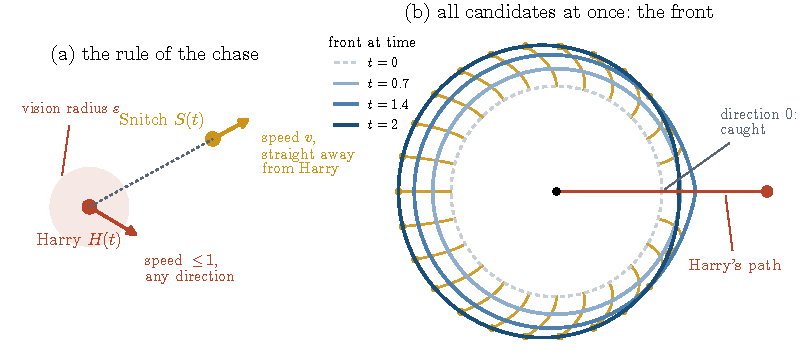
\includegraphics[width=\linewidth]{figs/fig_problem.pdf}
\caption{(a) The rule: the Snitch always flees straight away from Harry. (b) Harry does not know where the Snitch
started, so he faces one candidate for each direction (gold tracks, here while Harry runs straight to the right, with
the exaggerated speed $v=0.25$). Together the candidates form a closed curve, the \emph{front}, which swells and bends
as Harry moves. The fronts shown are those of the regularised candidates of Section~\ref{sec:virtual} (with
$\varepsilon=0.04$), which pass smoothly through direction~$0$; the front of the true candidates has a hole there,
because candidate~$0$ is caught.}
\label{fig:problem}
\end{figure}

\textbf{An easy case, and the real difficulty.} If $(1+2\pi)v\le\varepsilon/d$, Harry simply runs to the circle and once
around it: he passes the starting point of each candidate before time $(1+2\pi)d$, when that candidate has moved less
than $(1+2\pi)vd\le\varepsilon$, so he sees it. This argument says nothing when $\varepsilon$ is small compared with
$v$, and that is the interesting regime: we want a speed range for the Snitch, and a search time, that do not depend on
$\varepsilon$ at all. If that is possible, a limiting argument even lets Harry \emph{catch} the Snitch ($\varepsilon=0$).

\begin{theorem}[Uniform-in-$\varepsilon$ search]\label{thm:main}
There exist absolute constants $v_0>0$, $T_0>0$ and $\varepsilon_*>0$ such that for every $d>0$, every
$\varepsilon\in(0,d)$ and every $v\in(0,v_0]$ the explicit path $H=H_{v,\varepsilon,d}$ --- Design~T
\textup{(Definition~\ref{def:designT})} followed by the greedy chase \textup{(Definition~\ref{def:chase})} on the
working front of Theorem~\ref{thm:touchdown}, both run at vision radius $\varepsilon':=\min(\varepsilon,\varepsilon_*d)$
and scaled by $d$ --- satisfies $H(0)=0$, $|H'|\le1$ a.e., and for every $\alpha\in[0,2\pi)$ there is $t\le T_0d$
with $|S_\alpha(t)-H(t)|\le\varepsilon$.
\end{theorem}

\begin{corollary}[Exact catch]\label{cor:exact}
For every $d>0$ and $v\in(0,v_0]$ there is a $1$-Lipschitz path $H$ with $H(0)=0$ such that for every
$\alpha\in[0,2\pi)$ there is $t\le T_0d$ with $S_\alpha(t)=H(t)$.
\end{corollary}

The theorem is proved at the end of Section~\ref{sec:assembly} (any $T_0\ge15$ works), the corollary in
Section~\ref{sec:exact}. We do not try to make $v_0$ explicit: it is ``small enough that finitely many error terms of
size $O(v)$ fit under fixed margins''. A companion paper with the same architecture \cite{short} tracks every constant
and obtains $v_0=5.8\cdot10^{-3}$ and $T_0=13.1$, at the price of about fifty pages and one computer-checked constant.
Simulations (such as Figure~\ref{fig:designT}, where $v=0.1$) suggest that the same path works for much larger $v$.

\textbf{How the proof goes.} The candidates form a closed curve, the \emph{front}; Harry sees a candidate when he comes
within $\varepsilon$ of its point on the front. So Harry must sweep a curve whose points run away from him. Our path
(Section~\ref{sec:idea}) has two parts. \emph{Design~T}: Harry runs straight through the front, then turns and runs
along a straight line that just grazes the rest of it. \emph{The walk}: from the grazing point he walks along the
front in short straight legs, each aimed at the point an arclength $\varepsilon$ further on, and sees everything he
passes. The walk takes a bounded time provided the front stays nearly straight on every scale between $\varepsilon$
and a fixed length, and the heart of the proof is a bootstrap showing exactly this (Section~\ref{sec:chase}). It is
measured by the \emph{bendiness} of a pair of points, arclength minus chord (Section~\ref{sec:virtual}). The bootstrap
needs good starting data, which the grazing touch-down provides (Section~\ref{sec:touchdown}). One end of the front is
left close behind Harry at touch-down; we show that it stays straight while he walks away from it
(Section~\ref{sec:assembly}). Finally the time bound does not depend on $\varepsilon$, so we can let $\varepsilon\to0$
(Section~\ref{sec:exact}).

The main text states every result and proves the short ones. The three long arguments are in the appendices: the
bootstrap (Appendix~A), the shape of the front at touch-down (Appendix~B), and the departure from the tail end together
with the assembly (Appendix~C).

\textbf{Notation.} For $a,b\in\R^2=\C$: $a\cdot b:=\operatorname{Re}(\bar ab)$, $a\times b:=\operatorname{Im}(\bar ab)$
and $a^\perp:=ia$, so that $a^\perp\cdot b=a\times b$. We write $\mu:=v/(1-v)$ and $\mu_T:=3v/(1+v)$ (both are
$O(v)$; $\mu_T$ is the small loss in the flatness exponent of the front at touch-down, Theorem~\ref{thm:touchdown}).
From Section~\ref{sec:virtual} on, $d=1$ (except in the scaling step at the end of Section~\ref{sec:assembly}).
Throughout, $C,c$ denote positive constants that depend only on the locked numbers below (and on the absolute constants
of Theorem~\ref{thm:touchdown}), never on $R$, $v$ or $\varepsilon$; dependence on $R$ is written explicitly, as in
$O_R(v)$ (a quantity bounded by $C(R)\,v$).

\takeaway{Locked numbers}{%
The proof uses a handful of fixed numbers. Nothing depends on getting them optimal; they are fixed once and for all so
that no choice depends on a later one. With their roles (made precise where they are used):
$\gamma:=\frac23$ (flatness exponent of the walk), $\gamma_D:=\frac34$ (the same on its first stretch),
$\nu:=\frac1{24}$ (exponent of a weight that absorbs a logarithm), $\kappa:=\frac54$ (allowed stretch of a pair),
$c_A:=\frac12$ (allowed shortening of chords), $K_f:=10$ (near/far threshold, in pair lengths), $K_R:=12$ (cap on gaps,
in units of $R$), $c_{\mathrm{off}}:=\frac12$ (offset threshold for far pairs, in units of $R$), $K_\varepsilon:=10$
($\varepsilon\le R/K_\varepsilon$), $d_L:=2$ (a leg lasts at most $d_L\varepsilon$), $\delta_1:=\frac54$ (stretch factor
during one leg), $s_0:=\frac18$ (start bendiness), $A_0:=2$ (amplification allowed for far pairs), $f_F:=\frac12$
(bendiness of far pairs), and $m:=\frac1{10}$ (size of the bendiness bound).
Four more scales are chosen later, in the strict order $\lambda_0\to R\to v_0\to\varepsilon_*$: a scale $\lambda_0$
below which the front at touch-down is known to be flat (Section~\ref{sec:touchdown}), a small length $R$ up to which
the walk controls the bendiness, the speed threshold $v_0$, and the threshold $\varepsilon_*$ for the vision radius.
The precise conditions, the \emph{Parameter Lock}, are stated in Section~\ref{sec:assembly}, where all the objects they
refer to have been defined.}

}{}
\IfFileExists{main2.tex}{% main2.tex -- H-main.  Section 2: the idea in pictures.
%======================================================================
\section{The idea in pictures}\label{sec:idea}
%======================================================================

Harry's task is to pass within $\varepsilon$ of every point of the front (Figure~\ref{fig:problem}(b)), a closed curve
whose points all run away from him at speed $v$. Our path does this in two acts.

\begin{definition}[Design~T]\label{def:designT}
Let $d=1$ and $t_1:=1/(1-v)+1=2+\mu$.
\begin{itemize}
\setlength{\itemsep}{1pt}\setlength{\parskip}{0pt}
\item \textbf{Run 1:} $P(t):=t$ for $0\le t\le t_1$.
\item \textbf{Run 2:} Let $\alpha_0:=\arccos(v+1/t_1)$ and write $S_{\alpha_0}(t_1)-P(t_1)=\rho_0e^{i\beta^*}$; put
$\hat n:=e^{i\beta^*}$. Set $P(t):=P(t_1)+(t-t_1)\hat n$ for $t_1\le t\le t_\td$, where
\[
t_a:=t_1+\frac{\rho_0-\varepsilon}{1-v},\qquad t_\td:=t_a+\varepsilon\int_0^1\frac{d\sigma}{1-v\sigma(2-\sigma)},
\qquad t_c:=t_1+\frac{\rho_0}{1-v}.
\]
\end{itemize}
\end{definition}

In words: Harry first runs straight through the front and a distance $1$ beyond it, catching direction $0$ on the way.
He then runs straight at the candidate $\alpha_0$, which is chosen so that his line of approach is \emph{tangent} to the
front (at $v=0$ the front is the unit circle and run~2 is the tangent from the point $2$ to $e^{i\pi/3}$). The time
$t_\td$, the \emph{touch-down}, is the moment Harry reaches the regularised version of candidate $\alpha_0$
(Section~\ref{sec:virtual}): $t_a$ is when he arrives within $\varepsilon$ of it, and the integral is the exact time the
remaining distance $\varepsilon$ takes when that candidate flees with the reduced speed of Definition~\ref{def:F}
($t_c$ is when he would meet the true candidate $\alpha_0$; it is used only in Appendix~B). After
touch-down Harry \emph{walks the front}: he repeatedly runs straight at the point of the front an arclength
$\varepsilon$ further along, until he has passed all of it (Definition~\ref{def:chase}). Figure~\ref{fig:designT} shows
the whole path, computed numerically.

\begin{figure}[!htbp]
\centering
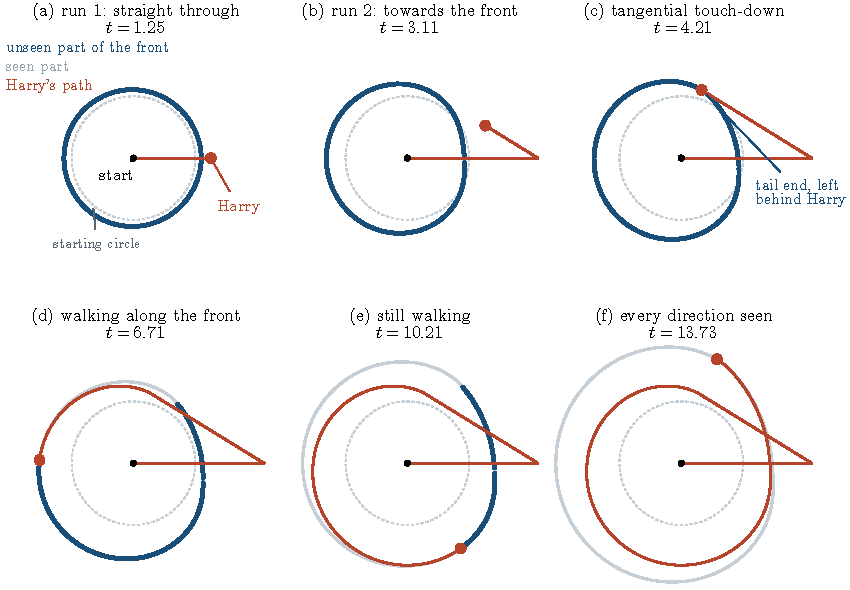
\includegraphics[width=0.98\linewidth]{figs/fig_designT.pdf}
\caption{The path of the proof, simulated for $v=0.1$ and $\varepsilon=0.02$. Harry (red) runs through the front, turns,
touches it tangentially, and then walks along it. The unseen part of the front is dark blue; the seen part fades to
grey. All directions are seen at $t\approx13.7$ (for $v\le v_0$ the proof gives $15$). As $v=0.1$ is not small, the
touch-down point is not $e^{i\pi/3}$ (its $v=0$ position) but about $0.33+1.10i$, at polar angle about $73^\circ$; the
candidate met there has direction $\alpha_0\approx55^\circ$. The simulation walks the whole front of regularised
candidates, including the sliver seen at touch-down and the labels near direction~$0$; the proof cuts that sliver off and
uses true candidates and the point $Z_s$ (Theorem~\ref{thm:touchdown}). So this is a close variant of the path of
Theorem~\ref{thm:main}.}
\label{fig:designT}
\end{figure}

\textbf{Why the walk can take bounded time.} Walking along a nearly straight piece of curve costs about its length, and
each leg sees everything it passes. The front has length about $2\pi$ and, as long as it stays nearly straight near
Harry, it does not grow much during the walk. So the walk should take a bounded time. The danger is \emph{bending at
small scales}: the candidates closest to Harry are pushed in quickly changing directions, and if the front crinkled at
scale $\varepsilon$, every leg would gain little and the walk could take a time growing with $1/\varepsilon$. The proof
must show that the front stays flat at every scale between $\varepsilon$ and a fixed length $R$, uniformly in
$\varepsilon$ --- with constants that do not get worse as $\varepsilon\to0$.

\textbf{Why not simply stop at first contact?} The obvious start is to run straight at the front and begin walking as
soon as some candidate is seen. Near that point the front then has a \emph{corner}: the candidates on either side were
pushed sideways by Harry's approach, so the two sides meet at an angle $2\arcsin v$ away from a straight line. Whichever
side Harry walks first, he leaves the other side behind him, and its end sits right next to his starting point. Harry
then runs away from it, and the exact motion on a straight run (Section~\ref{sec:touchdown}) shows what happens: the
left-behind end bends into a \emph{hook} whose direction keeps turning as one zooms in (Figure~\ref{fig:hook}(a)),
towards the direction perpendicular to Harry's path. On the piece of label length $\delta$ at the end, its relative
bendiness (the average angle between the arc and its chord) decays only like $\delta^{v/(1+v)}$ as $\delta\to0$, far
more slowly than the decay like $\delta^{\gamma}$, $\gamma=\frac23$, that the bootstrap requires
(Section~\ref{sec:virtual}). (Simulations suggest
that Harry still wins from such a start, through a delicate self-correcting balance, but we know no proof of that.)

\begin{figure}[!htbp]
\centering
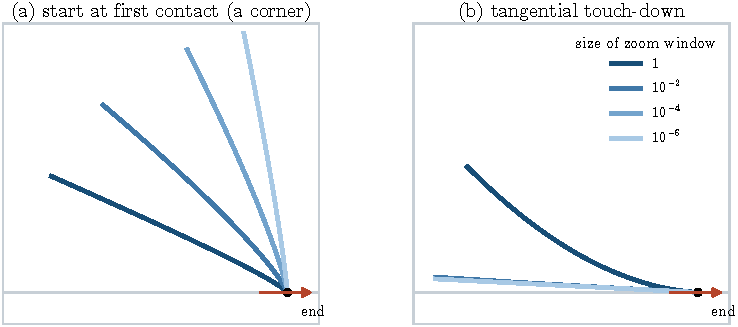
\includegraphics[width=0.92\linewidth]{figs/fig_hook.pdf}
\caption{A \emph{model arm} of the front, left behind by Harry as he runs off to the right, at time $1$ after he leaves
it ($v=0.2$, true candidates, exact straight-run motion). Each curve is the same end, seen through a zoom window of the
indicated size and magnified to unit size. (a) Start at first contact, idealised with $\varepsilon=0$: a straight ray at
the angle $2\arcsin v$ to Harry's backward direction, ending exactly at Harry. The end hooks: the finer the zoom, the
more it has turned (towards the perpendicular of Harry's path). (b) Tangential start: the parabola $y=s^2/2$ tangent to
Harry's path, ending $0.03$ behind him. Its end looks straight at every fine scale (automatic for a curve analytic at
positive distance from Harry; the comparison with (a) concerns $\varepsilon\to0$ with the tail end at distance
$z_0\gg\varepsilon$, as in Theorem~\ref{thm:touchdown}); only at scale $1$ does one see the curvature of the arm.}
\label{fig:hook}
\end{figure}

\textbf{The tangential touch-down.} Design~T avoids the corner. On run~2 Harry grazes the front along a tangent line, so
he sees only a thin sliver of candidates, of length about $\varepsilon^{1/2}$, and the front at touch-down is a smooth
curve tangent to his heading at both of its ends (Figure~\ref{fig:touchdown} in Section~\ref{sec:touchdown}). The end
he leaves behind is again close to him, at distance of order $\varepsilon^{1/2}$, but it is \emph{straight}, pointing
back along his path, and it stays straight while he walks away from it (Figure~\ref{fig:hook}(b),
Theorem~\ref{thm:departure}). The price is a little bookkeeping: pairs of points near that end are ``excused'' from the
bootstrap until Harry has walked a fixed distance $\We$; after that they are far from him and have exactly the starting
data the bootstrap needs.
}{}
\IfFileExists{main3.tex}{% main3.tex -- H-main.  Section 3: modified candidates and bendiness; basic lemmas with proofs.
%======================================================================
\section{Modified candidates and the bendiness of a pair}\label{sec:virtual}
%======================================================================

A real candidate has no well-defined velocity once Harry reaches it, and the front of real candidates tears where
candidates are caught. We therefore follow \emph{modified} (``virtual'') candidates, which slow down inside the vision
disc instead of fleeing at full speed. They agree with the real candidates until the moment they are seen, so seeing
every modified candidate is as good as seeing every real one; and their front is a smooth curve for all time, which never
shrinks. Then we introduce the quantity that measures how bent the front is, and derive the few calculus facts about it
that the rest of the proof uses. Throughout, $P$ is a $1$-Lipschitz path with $P(0)=0$, $d=1$ and $0<\varepsilon<1$.

\subsection{The regularised field and virtual fronts}

\begin{definition}[Regularised field]\label{def:F}
Put $f(\rho):=1$ for $\rho\ge\varepsilon$ and $f(\rho):=(\rho/\varepsilon)(2-\rho/\varepsilon)$ for
$0\le\rho\le\varepsilon$. Define $F(x):=f(|x|)\,x/|x|$ for $x\ne0$, $F(0):=0$, $A:=DF$, and $a^*(\rho):=1/\rho$ for
$\rho\ge\varepsilon$, $a^*(\rho):=2/\varepsilon$ for $\rho<\varepsilon$.
\end{definition}

\begin{lemma}\label{lem:F}
\textup{(i)} $F\in C^1(\R^2)$, $|F|\le1$, and $F(x)=x/|x|$ for $|x|\ge\varepsilon$.
\textup{(ii)} With $\rho=|x|$, $\hat r=x/\rho$ and $\Pi=I-\hat r\hat r^{\mathsf T}$:
$A=f'(\rho)\hat r\hat r^{\mathsf T}+(f(\rho)/\rho)\Pi$ is symmetric, $0\le A\le a^*(\rho)I$, $A=\Pi/\rho$ for
$\rho\ge\varepsilon$, $A(0)=(2/\varepsilon)I$, and $f(\rho)/\rho-f'(\rho)=\rho/\max(\rho,\varepsilon)^2$.
\textup{(iii)} For every unit vector $e$: $|e^\perp\cdot A(x)e|\le|x\times e|/\max(\rho,\varepsilon)^2$.
\textup{(iv)} $(F(x)-F(y))\cdot(x-y)\ge0$ for all $x,y$, and $(x/|x|-y/|y|)\cdot(x-y)\ge0$ for $x,y\ne0$.
\end{lemma}

\begin{proof}
Write $F(x)=\sigma(|x|)x$ with $\sigma(\rho)=(2\varepsilon-\rho)/\varepsilon^2$ on $[0,\varepsilon]$ and $\sigma=1/\rho$ on
$[\varepsilon,\infty)$. Both pieces have value $1/\varepsilon$ and slope $-1/\varepsilon^2$ at $\varepsilon$, so $\sigma$ is
$C^1$ on $(0,\infty)$; near $0$, $F(x)=(2\varepsilon x-|x|x)/\varepsilon^2$ is $C^1$ with $DF(0)=(2/\varepsilon)I$. Also
$|F|=f=1-(1-\rho/\varepsilon)^2\le1$ inside the disc. This is (i). Differentiating, $DF=\sigma I+\rho\sigma'\hat r\hat
r^{\mathsf T}=(f/\rho)\Pi+f'\hat r\hat r^{\mathsf T}$, since $f=\rho\sigma$. For $\rho\ge\varepsilon$ the eigenvalues are
$1/\rho$ and $0$; for $\rho<\varepsilon$ they are $f/\rho=(2\varepsilon-\rho)/\varepsilon^2\in(1/\varepsilon,2/\varepsilon]$ and
$f'=2(\varepsilon-\rho)/\varepsilon^2\in[0,2/\varepsilon]$, and $f/\rho-f'=\rho/\varepsilon^2$. This is (ii). For (iii),
$e^\perp\cdot Ae=-(f/\rho-f')(e\cdot\hat r)(e^\perp\cdot\hat r)$ and $|e^\perp\cdot\hat r|=|x\times e|/\rho$; use (ii).
For (iv), $(F(x)-F(y))\cdot(x-y)=\int_0^1(x-y)\cdot A(y+s(x-y))(x-y)\,ds\ge0$; and
$(x/|x|-y/|y|)\cdot(x-y)=|x|+|y|-(x\cdot y)(1/|x|+1/|y|)\ge0$ because $x\cdot y\le|x||y|$.
\end{proof}

\begin{definition}[Virtual flow]\label{def:vflow}
Given a $C^1$ curve $x^\circ:[u_-,u_+]\to\R^2$ with $\partial_ux^\circ\ne0$ and a time $t_\circ\ge0$, the
\emph{virtual flow} of $P$ from $x^\circ$ at $t_\circ$ solves
\[
\partial_tx(u,t)=vF\bigl(x(u,t)-P(t)\bigr),\qquad x(u,t_\circ)=x^\circ(u),\qquad t\ge t_\circ .
\]
We write $x_u(t):=x(u,t)$, $r=r_u:=x-P$, $\rho:=|r|$, $\hat r:=r/\rho$, $w:=|\partial_ux|$,
$T:=\partial_ux/w=e^{i\psi}$ and $\phi:=\arg r-\psi$. \emph{Virtual candidates} $x_\theta(t)$ start at $t_\circ=0$ from
$x^\circ(\theta)=e^{i\theta}$. A \emph{working front} starts at $t_\circ=t_\td$ from a curve $x^0$ on $[0,U]$ with
$|\partial_ux^0|\equiv1$; a label $u$ of it is \emph{true with direction $\theta$} if $S_\theta$ exists on $[0,t_\td]$
and $x^0(u)=S_\theta(t_\td)$.
\end{definition}

\begin{lemma}[Basic properties of virtual flows]\label{lem:vflow}
For a virtual flow:
\textup{(a)} $x(\cdot,t)$ is $C^1$, $|\partial_tx|\le v$, $\partial_t\partial_ux=vA(r)\partial_ux$, and both $w$ and
the arclengths $l(a,b;t)=\int_a^bw\,du$ are non-decreasing in $t$ \textup(so $w\ge1$ on a working front\textup).
\textup{(b)} $w_t=vw\,T\cdot AT$, $T_t=v(AT-(T\cdot AT)T)$ and
$\psi_t=-v\rho\max(\rho,\varepsilon)^{-2}\sin\phi\cos\phi$. For $\rho\ge\varepsilon$: $w_t/w=v\sin^2\phi/\rho$ and
$\psi_t=-(v/\rho)\sin\phi\cos\phi$.
\textup{(c)} For fixed labels, $l$, $c$ and $E$ \textup(the latter two where $c>0$; Definition~\ref{def:twopt}\textup)
are $C^1$ in $t$, and their derivatives depend on $P$ only through $P(t)$.
\end{lemma}

\begin{proof}
The field $(t,x)\mapsto vF(x-P(t))$ is continuous, and $C^1$ in $x$ with $|D_x|\le2v/\varepsilon$ (Lemma~\ref{lem:F}).
By the standard theory \cite[Ch.~V]{Hartman}, solutions are global and unique, depend $C^1$ on the initial point, and
$\partial_ux$ solves the variational equation $\partial_t\partial_ux=vA(r)\partial_ux$. Hence
$\partial_t(w^2)=2v\,\partial_ux\cdot A\partial_ux\ge0$, which gives (a) and $w_t=vwT\cdot AT$. Then
$T_t=(\partial_ux)_t/w-\partial_ux\,w_t/w^2$ is the formula in (b), and $\psi_t=T^\perp\cdot T_t=vT^\perp\cdot AT$.
Lemma~\ref{lem:F}(iii) with $e=T$ (where $T\cdot\hat r=\cos\phi$, $T^\perp\cdot\hat r=\sin\phi$) gives $\psi_t$; for
$\rho\ge\varepsilon$, $T\cdot AT=T\cdot\Pi T/\rho=\sin^2\phi/\rho$. Part (c) follows since $w>0$ and $\partial_ux$ is
$C^1$ in $t$, and the time derivatives are integrals of $vA(x-P(t))\partial_ux$.
\end{proof}

\begin{lemma}[Virtual hits imply true sightings]\label{lem:seen}
If $\rho_\theta(t)\le\varepsilon$ for a virtual candidate, or $\rho_u(t)\le\varepsilon$ for a true label $u$ of a working
front with direction $\theta$ and some $t\ge t_\td$, then the true candidate $S_\theta$ is seen by time $t$.
\end{lemma}

\begin{proof}
Let $t'\le t$ be the first time at which $\rho\le\varepsilon$ (it exists by continuity; for a virtual candidate $t'>0$
since $\rho(0)=1>\varepsilon$). Up to $t'$ we have $\rho\ge\varepsilon$, hence $F(x-P)=(x-P)/\rho$: the virtual point
solves the true equation \eqref{eq:snitch}. By uniqueness for \eqref{eq:snitch} away from $H$, it coincides with
$S_\theta$ on $[0,t']$ (respectively on $[t_\td,t']$, where it starts from $S_\theta(t_\td)$). So $S_\theta$ exists up to
$t'$ and $|S_\theta(t')-P(t')|=\rho(t')\le\varepsilon$.
\end{proof}

\begin{lemma}[Chords never shrink]\label{lem:chords}
Let $X_a,X_b$ solve $X'=vV(X-P)$ on $[t_1,t_2]$, each with its own $V\in\{F,\,x\mapsto x/|x|\}$ \textup(for $x/|x|$,
as long as the point does not meet $P$\textup).
\textup{(a)} If both use $F$, then $|X_b-X_a|$ is non-decreasing; in particular, chords $c(a,b;t)$ of a virtual flow are
non-decreasing in $t$.
\textup{(b)} In general, if $|X_b(t_1)-X_a(t_1)|\ge2\varepsilon$, then $|X_b(t)-X_a(t)|\ge|X_b(t_1)-X_a(t_1)|$ on
$[t_1,t_2]$.
\end{lemma}

\begin{proof}
Put $p_a:=X_a-P$, $p_b:=X_b-P$ and $D:=X_b-X_a=p_b-p_a$. Then $(|D|^2)'=2v(V_b(p_b)-V_a(p_a))\cdot(p_b-p_a)$. If
$V_a=V_b$ this is $\ge0$ by Lemma~\ref{lem:F}(iv), which proves (a). For (b), note first: whenever $|D|\ge2\varepsilon$,
one of $|p_a|,|p_b|$ is at least $\varepsilon$, say $|p_b|$; there $V_b(p_b)=p_b/|p_b|=F(p_b)$, and $V_b(p_b)-V_a(p_a)$
is a difference of the single monotone field $F$ (if $V_a=F$) or $x/|x|$ (if $V_a=x/|x|$), so again $(|D|^2)'\ge0$.
Now if $|D(t_1)|>2\varepsilon$, let $\tau$ be the infimum of times with $|D|<|D(t_1)|$; if $\tau<t_2$, then
$|D|>2\varepsilon$ on a neighbourhood of $\tau$, where $|D|$ is non-decreasing, a contradiction. If
$|D(t_1)|=2\varepsilon$, replace $X_b(t_1)$ by $X_b(t_1)+\iota D(t_1)/|D(t_1)|$; the perturbed solutions exist on
$[t_1,t_2]$ for small $\iota>0$, keep distance $\ge2\varepsilon+\iota$ from $X_a$, and converge to $X_b$ as $\iota\to0$.
\end{proof}

\subsection{Bendiness: arc minus chord}

How do we measure ``nearly straight''? Take two points $x_a,x_b$ on the front. The arc between them has length $l$, the
straight segment has length $c$, and the difference $E=l-c\ge0$ vanishes exactly when the arc is straight. We use
$N:=\sqrt{2E}$, because of a simple identity (Lemma~\ref{lem:excess}(b)): $N^2=\int|T-e|^2\,ds$, where $e$ is the
direction of the chord. So $N/\sqrt l$ is the root-mean-square angle between the front and its chord. The bound the proof
maintains, $N\le M\lambda^{1/2+\gamma}$ with $M\lambda^\gamma=m(\lambda/R)^\gamma$ (here $\gamma=\frac23$ and
$m=\frac1{10}$ are locked numbers, $R$ is a fixed small length chosen in Section~\ref{sec:assembly}, and
$M:=mR^{-\gamma}$), says: \emph{on a piece of label
length $\lambda$, the front deviates from its chord by an average angle at most $m(\lambda/R)^{\gamma}$}, which tends
to zero as the piece shrinks. Figure~\ref{fig:bend} shows the quantities; whether a pair is ``near'' or ``far'' depends
on its distance from Harry measured in units of its own length.

\begin{figure}[!htbp]
\centering
\begin{tikzpicture}[scale=1.0,>=Stealth]
  % left: one pair
  \begin{scope}[shift={(0,0)},scale=1.15]
    \draw[primary!35,line width=1pt] (-0.5,-0.4) .. controls (0.2,0.5) and (1.3,1.3) .. (2.2,1.35)
       .. controls (3.1,1.4) and (3.9,0.7) .. (4.5,-0.3);
    \draw[primary,line width=2.2pt] (0.32,0.5) .. controls (0.9,1.1) and (1.5,1.33) .. (2.2,1.35)
       .. controls (2.9,1.37) and (3.3,1.0) .. (3.65,0.62);
    \fill[primary] (0.32,0.5) circle (2pt) node[left,font=\small] {$x_a$};
    \fill[primary] (3.65,0.62) circle (2pt) node[right,font=\small] {$x_b$};
    \draw[accent,thick,dashed] (0.32,0.5) -- (3.65,0.62) node[pos=0.62,below,font=\small] {chord $c$};
    \node[primary,font=\small] at (2.2,1.68) {arc $l$};
    \draw[->,thick,black!70] (0.75,0.96) -- ++(0.55,0.45) node[above,font=\footnotesize] {$T$};
    \draw[->,thick,black!70] (0.75,0.96) -- ++(0.75,0.027) node[right,font=\footnotesize] {$e$};
    \node[font=\small,align=center] at (2.0,-0.8) {bendiness: $E=l-c$, \ $N=\sqrt{2E}$,\\[2pt]
      $N^2=\int_a^b|T-e|^2\,ds$};
  \end{scope}
  % right: near and far pairs relative to Harry on a leg
  \begin{scope}[shift={(6.4,0)},scale=1.0]
    \draw[primary!35,line width=1pt] (0,0) .. controls (2.0,0.18) and (3.8,0.30) .. (6.0,0.55)
      .. controls (7.0,0.68) and (8.0,0.88) .. (9.0,1.12);
    \coordinate (Aj) at (0.5,0.04);
    \coordinate (P) at (1.1,0.09);
    \coordinate (Aj1) at (1.7,0.15);
    \draw[accent,very thick] (Aj) -- (P);
    \draw[accent,thick,dashed] (P) -- (Aj1);
    \fill[accent] (P) circle (2.4pt) node[above=2pt,font=\small] {Harry};
    \fill[primary] (Aj) circle (1.6pt);
    \fill[primary] (Aj1) circle (1.6pt);
    \node[font=\footnotesize,primary] at (0.5,-0.25) {$x_{a_j}$};
    \node[font=\footnotesize,primary] at (1.85,-0.15) {$x_{a_{j+1}}$};
    % near pair
    \draw[primary,line width=2.2pt] (2.3,0.2) .. controls (2.7,0.23) and (3.1,0.26) .. (3.4,0.29);
    \node[font=\footnotesize,primary,align=center] at (2.85,0.75) {near pair\\(gap $<K_f\lambda$)};
    % far pair
    \draw[primary,line width=2.2pt] (6.6,0.63) .. controls (6.9,0.67) and (7.2,0.72) .. (7.5,0.79);
    \node[font=\footnotesize,primary,align=center] at (6.9,1.4) {far pair\\(gap $\ge K_f\lambda$)};
    \draw[<->,muted] (0.5,-0.6) -- (6.6,-0.6) node[midway,below,font=\footnotesize] {gap $g=a-a_j$};
    \draw[<->,muted] (6.6,-0.6) -- (7.5,-0.6) node[midway,below,font=\footnotesize] {$\lambda$};
  \end{scope}
\end{tikzpicture}
\caption{Left: the bendiness of a pair of points is the arc length minus the chord length; it is zero exactly for a
straight piece. Right: Harry walks the front in short legs; a pair is \emph{near} if its distance ahead of Harry is less
than ten times its own length, and \emph{far} otherwise (legs, the base point $x_{a_j}$ and the gap $g$ are defined in
Section~\ref{sec:chase}).}
\label{fig:bend}
\end{figure}

\begin{definition}[Two-point quantities]\label{def:twopt}
For a regular $C^1$ curve $u\mapsto x_u$ (arclength element $ds=w\,du$) and labels $a<b$:
\[
l(a,b):=\int_a^bds,\;\; c(a,b):=|x_b-x_a|,\;\; E:=l-c\ge0,\;\; N:=(2E)^{1/2},\;\; e=e_{ab}:=\frac{x_b-x_a}{c}\;\;(c>0).
\]
Set $\varsigma:=T\cdot e^\perp$, $q:=e^\perp\cdot A(r)e$, and, for a unit vector $\hat u$ and an interval $J$,
$V_{\hat u}(J):=\int_J|T-\hat u|^2\,ds$ and $\mathbf v_J:=x_{b'}-x_{a'}=c(J)e_J$ for $J=(a',b')$.
\end{definition}

\begin{lemma}[Excess and curvature]\label{lem:excess}
For a regular $C^1$ curve and an interval $J=(a,b)$:
\textup{(a)} $E(a',b')\le E(a,b)$ for $a\le a'<b'\le b$.
\textup{(b)} $V_{\hat u}(J)=2[l(J)-(x_b-x_a)\cdot\hat u]=N(J)^2+c(J)|e_J-\hat u|^2$ \textup(if $c(J)>0$\textup). Thus
$\int_J|T-e_J|^2\,ds=N(J)^2$, $V_{\hat u}$ is additive over adjacent intervals, and
$|\hat u\times(x_b-x_a)|\le(l\,V_{\hat u})^{1/2}$.
\textup{(c)} If the tangent angle is $K$-Lipschitz in arclength on $J$ and $Kl\le\pi$, then $N\le(K/\sqrt{12})\,l^{3/2}$.
\end{lemma}

\begin{proof}
(a) $l(a,b)=l(a,a')+l(a',b')+l(b',b)$ while $c(a,b)\le l(a,a')+c(a',b')+l(b',b)$. (b) $|T-\hat u|^2=2-2T\cdot\hat u$ and
$\int_JT\,ds=x_b-x_a=c\,e_J$, so $V_{\hat u}=2l-2c\,e_J\cdot\hat u=2(l-c)+c(2-2e_J\cdot\hat u)$. Also
$\hat u\times(x_b-x_a)=\int_J\hat u\times(T-\hat u)\,ds$; apply Cauchy--Schwarz. (c) With $\psi_m$ the tangent angle at
the midpoint, $|\psi(s)-\psi_m|\le K|s-l/2|\le\pi/2$, so
$c\ge\int_0^l\cos(\psi-\psi_m)\,ds\ge\int_0^l\cos(K|s-l/2|)\,ds=\frac2K\sin\frac{Kl}2\ge l-\frac{K^2l^3}{24}$.
\end{proof}

The next lemma says that a short piece inside a nearly straight longer piece points in nearly the same direction.

\begin{lemma}[Split tilt]\label{lem:splittilt}
For intervals $J\subset I$, $J\ne I$, with $c(I),c(J)>0$, put $l_c:=l(I)-l(J)$ and $Z:=|\mathbf v_J\times e_I|$. Then
\textup{(i)} $Z^2\le N(I)^2\,l(J)\,l_c/l(I)$;
\textup{(ii)} if $N(I)^2<4c(J)$, then $|e_J-e_I|\le(Z/c(J))\bigl(1-N(I)^2/(4c(J))\bigr)^{-1/2}$.
\end{lemma}

\begin{proof}
(i) $\mathbf v_J\times e_I=\int_J(T-e_I)\times e_I\,ds$, and also $=-\int_{I\setminus J}(T-e_I)\times e_I\,ds$ since
$\mathbf v_I\times e_I=0$. Cauchy--Schwarz gives $Z^2\le l(J)\int_J|T-e_I|^2$ and $Z^2\le l_c\int_{I\setminus J}|T-e_I|^2$.
Divide by $l(J)$ and $l_c$, add, and use Lemma~\ref{lem:excess}(b): $Z^2\,l(I)/(l(J)l_c)\le N(I)^2$.
(ii) With $\mathbf d:=e_J-e_I$, $|\mathbf d|^2(1-|\mathbf d|^2/4)=|e_J\times e_I|^2=Z^2/c(J)^2$, and
Lemma~\ref{lem:excess}(b) gives $c(J)|\mathbf d|^2\le V_{e_I}(J)\le V_{e_I}(I)=N(I)^2$.
\end{proof}

\subsection{How the bendiness changes in time}

The next lemma computes the time derivative of the bendiness of a fixed pair. Its last part is the key estimate for
pairs far from Harry: there the field $x/|x|$ is smooth on the scale of the pair, and the bendiness can grow only
through the sideways offset $p_a$ of Harry from the chord.

\begin{lemma}[Evolution of $l$, $c$ and $E$]\label{lem:Eprime}
For a virtual flow, fixed labels $a<b$ and $c(a,b;t)>0$ \textup(integrals over the arc from $x_a$ to $x_b$\textup):
\begin{enumerate}[(i)]
\setlength{\itemsep}{1pt}\setlength{\parskip}{0pt}
\item $l'=v\int T\cdot AT\,ds$ and $c'=v\int e\cdot AT\,ds$.
\item $E'=v\int(T-e)\cdot A(T-e)\,ds-\frac v2\int(e\cdot Ae)|T-e|^2\,ds+v\int\varsigma q\,ds$, where
$\int|T-e|^2\,ds=N^2$, $\int\varsigma\,ds=0$ and $|\varsigma|\le|T-e|$.
\item For every constant $\bar q$: $E'\le v\int a^*(\rho)|T-e|^2\,ds+v\int\varsigma(q-\bar q)\,ds$; also
$E'\le vN\|AT\|_{L^2(ds)}$.
\item \textup(Far inequality\textup) Let $\underline\rho:=\min_{s\in[a,b]}\rho_s$ and $p_a:=r_a\times e$. If
$\underline\rho\ge\varepsilon$, then
\[
E'\le\frac v{\underline\rho}\Bigl(1+\frac l{\pi\underline\rho}+\frac{2l^2}{\pi^2\underline\rho^2}\Bigr)N^2
+\frac{2vl^{3/2}|p_a|N}{\pi\underline\rho^3},\qquad
l'\le\frac v{\underline\rho}\Bigl[N+\frac{l^{1/2}|p_a|+lN/\pi}{\underline\rho}\Bigr]^2 .
\]
\end{enumerate}
\end{lemma}

\begin{proof}
(i) $l'=\int w_t\,du$ with Lemma~\ref{lem:vflow}(b); $c'=e\cdot\partial_t(x_b-x_a)=e\cdot\int_a^bvA\,\partial_ux\,du$.
(ii) $E'=v\int(T-e)\cdot AT$ ($A$ is symmetric). Write $(T-e)\cdot AT=(T-e)\cdot A(T-e)+(T-e)\cdot Ae$ and expand
$T-e=-\frac12|T-e|^2e+\varsigma e^\perp$ (as $T\cdot e=1-\frac12|T-e|^2$). Also $\int\varsigma\,ds=e^\perp\cdot(x_b-x_a)=0$.
(iii) Drop the middle term of (ii) ($A\ge0$), use $A\le a^*I$, and subtract $\bar q\int\varsigma=0$. The second bound is
Cauchy--Schwarz applied to $E'=v\int(T-e)\cdot AT$.
(iv) On the arc $\rho\ge\varepsilon$, so $A=\Pi/\rho$; the first term of (ii) is at most $vN^2/\underline\rho$. For the
last term use arclength $\sigma\in[0,l]$ from $x_a$ and coordinates $y=y_1e+y_2e^\perp$; then $q=Q(r)$ with
$Q(y)=-y_1y_2/|y|^3$, and a direct computation gives $|\partial_{y_2}Q|\le|y|^{-2}$ and $|\partial_{y_1}Q|\le2|y_2|/|y|^3$.
Let $\delta(\sigma):=\int_0^\sigma\varsigma$; then $\delta(0)=\delta(l)=0$, $|y_2(\sigma)|=|r_a\cdot e^\perp+\delta|\le|p_a|+|\delta|$,
and by Wirtinger's inequality \cite[Thm.~257]{HLP} $\int\delta^2\le(l/\pi)^2\int\varsigma^2\le(l/\pi)^2N^2$, hence
$\int|\delta|\le l^{3/2}N/\pi$. Integrating by parts (at a fixed time $dr/d\sigma=T$),
\[
\int\varsigma q\,d\sigma=-\int\delta\,\bigl(\partial_{y_1}Q\,(T\cdot e)+\partial_{y_2}Q\,\varsigma\bigr)\,d\sigma
\le\int|\delta|\frac{2(|p_a|+|\delta|)}{\underline\rho^3}+\int\frac{|\delta||\varsigma|}{\underline\rho^2}
\le\frac{2|p_a|l^{3/2}N}{\pi\underline\rho^3}+\frac{2l^2N^2}{\pi^2\underline\rho^3}+\frac{lN^2}{\pi\underline\rho^2},
\]
which gives the bound on $E'$. For $l'$: $T\cdot AT=\sin^2\phi/\rho$ with $|\sin\phi|=|T\times r|/\rho$ and
$|T\times r|\le|T-e|\rho+|e\times r|=|T-e|\rho+|y_2|$; so $|\sin\phi|\le|T-e|+(|p_a|+|\delta|)/\underline\rho$, and
Minkowski's inequality gives $(\int\sin^2\phi)^{1/2}\le N+(l^{1/2}|p_a|+lN/\pi)/\underline\rho$.
\end{proof}

\begin{lemma}[Duhamel inequality]\label{lem:duhamel}
If $c(a,b;t_1)>0$ and $\underline\rho(t)\ge\varepsilon$ on $[t_1,t_2]$, then with the \emph{rate}
$\mathcal A:=(v/\underline\rho)(1+l/(\pi\underline\rho)+2l^2/(\pi^2\underline\rho^2))$ and the \emph{forcing}
$\mathcal B:=2vl^{3/2}|p_a|/(\pi\underline\rho^3)$,
\[
N(t_2)\le e^{\int_{t_1}^{t_2}\mathcal A}N(t_1)+\int_{t_1}^{t_2}e^{\int_t^{t_2}\mathcal A}\mathcal B(t)\,dt .
\]
If moreover $\underline\rho\ge Kl$ on $[t_1,t_2]$, then $\mathcal A\le\mathcal A^*(K)\,v/\underline\rho$, where
$\mathcal A^*(K):=1+1/(\pi K)+2/(\pi K)^2$.
\end{lemma}

\begin{proof}
By Lemma~\ref{lem:chords}(a), $c\ge c(t_1)>0$ on $[t_1,t_2]$, so $E$ is $C^1$ there (Lemma~\ref{lem:vflow}(c));
$\mathcal A$ and $\mathcal B$ are continuous ($\underline\rho$ is a minimum of a jointly continuous function over a
compact label set). For $\iota>0$ put $N_\iota:=(N^2+\iota^2)^{1/2}$. By Lemma~\ref{lem:Eprime}(iv),
$N_\iota N_\iota'=E'\le\mathcal AN^2+\mathcal BN\le\mathcal AN_\iota^2+\mathcal BN_\iota$, so
$N_\iota'\le\mathcal AN_\iota+\mathcal B$. Integrate this linear inequality and let $\iota\to0$. The last claim is
$l/\underline\rho\le1/K$.
\end{proof}

}{}
\IfFileExists{main4.tex}{% main4.tex -- H-main.  Section 4: walking the front; the end theorem (proved in Appendix A).
%======================================================================
\section{Walking the front: the end theorem}\label{sec:chase}
%======================================================================

This section is about the second act alone. Suppose Harry stands on a smooth front that is nearly straight at every
small scale. He walks along it in legs: from his current point he aims at the point an arclength $\varepsilon$ further
on and runs straight at it until he meets it. Everything he passes is within $\varepsilon$ of him, so it is seen. The
end theorem says that, if the front is flat enough to begin with, it \emph{stays} flat for the whole walk, every leg
makes progress at least $\varepsilon/\kappa$ along the front, and the walk ends after a time comparable to the length
of the front. We first define the walk precisely; throughout, $x$ is a working front on $[0,U]$ started at $t_\td$
with $|\partial_ux^0|\equiv1$, and a \emph{pair} $(a,b)$, $a<b$, has \emph{label length} $\lambda:=b-a$.

\begin{definition}[Greedy chase]\label{def:chase}
Let $P$ be $1$-Lipschitz on $[0,t_\td]$ with $x^0(0)=P(t_\td)$, and fix a \emph{cut} $b_c\in(0,U]$. Set
$t_0:=t_\td$ and $a_0:=0$. Given a leg start $t_j$ with $P(t_j)=x_{a_j}(t_j)$, let
\[
a_{j+1}:=\max\bigl\{u\in[a_j,b_c]:\ l_{t_j}(a_j,u)\le\varepsilon\bigr\}.
\]
If $a_{j+1}=b_c$, the chase stops at $T_\stopp:=t_j$ (leg $j+1$ is \emph{final} and is not walked; $P$ stays constant
after $T_\stopp$). Otherwise $P$ runs at unit speed along the ray from $P(t_j)$ through $x_{a_{j+1}}(t_j)$ until it
meets $x_{a_{j+1}}$, at time $t_{j+1}$; this requires the \emph{proviso} $c(a_j,a_{j+1};t_j)>0$. Leg $j+1$ is the time
interval $[t_j,t_{j+1}]$ and its direction is $\hat u_{j+1}$. For $t\in(t_j,t_{j+1}]$ (and for $t=t_0$, with $j=0$),
the label $a_{j(t)}:=a_j$ is the \emph{base} at time $t$.
\end{definition}

During a leg the target point flees straight away from Harry along his line of motion, so he gains on it at rate at
least $1-v$ and a leg lasts at most $\varepsilon/(1-v)$; every true label between $a_j$ and $a_{j+1}$ is within
$\varepsilon$ of Harry at the leg start, hence seen. These and other basic facts about the chase are collected in
Lemma~\ref{lem:chase} (Appendix~A).

\textbf{The setting.} The end theorem is used twice (once on a short initial arc, once on the whole front), and it must
tolerate the excused pairs near the tail end mentioned in Section~\ref{sec:idea}. This is what the following setting
encodes. The admissible pairs are those of label length between $\varepsilon/2$ and $R$ that are still ahead of Harry.
On a first reading one may take $\We=0$: then there are no tail pairs, $\mathcal F_*=\mathcal F$ below, and (TW) is
void; the excused tail is needed only in Section~\ref{sec:assembly}.

\textbf{Setting (H).}\phantomsection\label{set:H} Fix the locked parameters (with either $\gamma=\frac23$ or
$\gamma=\gamma_D=\frac34$), $M:=mR^{-\gamma}$, $U\le U_0:=8$, $\varepsilon\le R/K_\varepsilon$, the chase of
Definition~\ref{def:chase} on the working front $x$ on $[0,U]$ \emph{with cut $b_c=U$}, and an \emph{excuse
length} $\We\ge0$ (either $\We=0$ or $U\ge2\We+R+\varepsilon$), together with a number $\delta_t\ge0$ (in the application
$\delta_t=O_R(v)$; only $\delta_t\le\frac1{16}$ is used). A pair $(a,b)\subset[0,U]$ is a \emph{body pair} if
$U-b\ge\We$, a \emph{tail pair} if $U-b<\We$, and \emph{good} if $a\ge\We$ or $U-b\ge\We$ (every pair with $\lambda\le R$
is good). The \emph{family} $\mathcal F(t)$ on leg $j+1$ consists of the pairs with $\varepsilon/2\le\lambda\le R$ and
($a=a_j$ or $a\ge a_{j+1}$); pairs starting strictly inside the current leg are left out because their first point was
within $\varepsilon$ of Harry at the leg start and is therefore already seen. The \emph{gap} of a family pair is
$g:=a-a_{j(t)}\ge0$, and the pair is \emph{far} if $g\ge K_f\lambda$ and \emph{near} otherwise. Let $j_W$ be the first $j$ with $a_j\ge\We$, and $t_W:=t_{j_W}$. The \emph{admissible
family} $\mathcal F_*(t)$ consists of the body pairs of $\mathcal F(t)$ for $t<t_W$, and of all of $\mathcal F(t)$ for
$t\ge t_W$. Assume:
\begin{itemize}
\setlength{\itemsep}{2pt}\setlength{\parskip}{0pt}
\item[(S1)] $c(a,b;t_\td)\ge c_A\min(\lambda,K_RR)$ for all good pairs with $\lambda\ge\varepsilon/2$;
\item[(S2)] $N(a,b;t_\td)\le s_0M\lambda^{1/2+\gamma}\min\bigl(1,\,K_f\lambda/\min(a,K_RR)\bigr)^\nu$ for all body
pairs with $\varepsilon/2\le\lambda\le R$;
\item[(TW)] (if $\We>0$ and $t_W$ is reached) every tail pair with $\varepsilon/2\le\lambda\le R$ satisfies, with
$g_W:=a-a_{j_W}$,
\[
g_W\ge K_f\lambda,\qquad l_{t_W}(a,b)\le(1+\delta_t)\lambda,\qquad
N(a,b;t_W)\le s_0M\lambda^{1/2+\gamma}\min\Bigl(1,\,\frac{K_f\lambda}{\min(g_W,K_RR)}\Bigr)^\nu .
\]
\end{itemize}
The weight $\min(\cdot)^\nu$ in (S2) and (TW) asks a pair that starts far ahead of Harry to be slightly flatter; this
pays for the logarithmic amplification $\int v\,dt/g$ that it suffers while Harry approaches (see ``Far pairs'' below).

\begin{theorem}[End theorem]\label{thm:end}
In Setting~\textup{(H)}, provided $v_0=v_0(m,R)>0$ is sufficiently small, the proviso holds at every non-final leg
start, and:
\begin{enumerate}[(a)]
\setlength{\itemsep}{1pt}\setlength{\parskip}{0pt}
\item \textup{(Invariants)} For all $t\in[t_\td,T_\stopp]$ and all $(a,b)\in\mathcal F_*(t)$,
\begin{equation}\label{eq:invariants}
\text{\textup{(J1)}}\quad l_t(a,b)\le\kappa\lambda,\qquad\text{\textup{(J2)}}\quad N(a,b;t)\le M\lambda^{1/2+\gamma};
\end{equation}
if $\We>0$, then $t_W$ is reached. Moreover $c(a,b;t)\ge c_A\min(\lambda,K_RR)$ for all good pairs with
$\lambda\ge\varepsilon/2$.
\item \textup{(Termination)} Every non-final leg advances the base by $a_{j+1}-a_j\in[\varepsilon/\kappa,\varepsilon]$;
the chase stops by $T_\stopp\le t_\td+\kappa U/(1-v)$; and every true label of $[0,U]$ is seen by $T_\stopp$.
\item \textup{(Tilts)} For $J\subset I$ in $\mathcal F_*(t)$: $|e_J-e_I|\le C_TM\lambda_I^\gamma$, with the absolute
constant $C_T:=\sqrt5\,(1-2m^2)^{-1/2}/(1-2^{-\gamma})$ \textup($C_T<6.11$ for $\gamma=\frac23$, $C_T<5.58$ for
$\gamma=\frac34$\textup).
\item \textup{(Distance from the base)} On leg $j+1$, for $s\ge a_j$ with $U-s\ge\We$ or $a_j\ge\We$:
$\rho_s(t)\ge c_A\min(s-a_j,K_RR)-\delta_1\varepsilon$ and $\max(\rho_s(t),\varepsilon)\ge\min(s-a_j,K_RR)/c_6$, where
$c_6:=(1+\delta_1)/c_A=\frac92$.
\item \textup{(Causality)} If $\tilde P=P$ on $[0,t_j]$, then \textup{(a)}, \textup{(c)}, \textup{(d)} hold for
$\tilde P$ on $[t_\td,t_j]$.
\end{enumerate}
\end{theorem}

The proof is in Appendix~A. Here is why it works.

\textbf{A first-failure argument.} The invariants (J1)--(J2) hold at $t_\td$ with room to spare, by (S1)--(S2). Both
sides change continuously in time, so if they ever fail there is a first moment when one of them becomes an equality.
It therefore suffices to show that, as long as (J1)--(J2) hold, they actually hold in the \emph{strictly stronger} forms
$l<\kappa\lambda$ and $N^2\le\bar\theta M^2\lambda^{1+2\gamma}$ for a fixed $\bar\theta<1$ (Lemma~\ref{lem:cont}). The
invariants are exactly what keeps the chase healthy: (J1) makes every leg advance the base by at least $\varepsilon/\kappa$,
so the walk ends in time about $\kappa U$; and (J2), via the split-tilt lemma, keeps all chords pointing in nearly the
same direction, so Harry is never far off the line of the pairs ahead of him. Three estimates give the strict forms.

\emph{Far pairs} (Proposition~\ref{prop:far}). A pair whose distance ahead of Harry is at least $K_f=10$ times its own
length sees Harry from far away. The regularisation plays no role there, and the far inequality and the Duhamel
inequality (Lemmas~\ref{lem:Eprime}(iv) and \ref{lem:duhamel}) apply. The amplification factor $\exp\int\mathcal A$
involves $\int v\,dt/g$, which grows only logarithmically as the gap $g$ shrinks; the factor $\min(\cdot)^\nu$ in (S2) is
designed to absorb exactly this logarithm. The forcing $\mathcal B$ is small because Harry is nearly on the line of the
pair: his sideways
offset $|p_a|$ is controlled by the bendiness of a longer pair reaching back to him. The result is
$N\le f_FM\lambda^{1/2+\gamma}$ with $f_F=\frac12$.

\emph{Near pairs} (Proposition~\ref{prop:near}). A pair close to Harry may feel the singular part of the field, but
only briefly: Harry moves past it at speed about $1$, so it is near for a time of order $\lambda$, and the integral of
the excess growth over that time is bounded by a constant times $vM^2\lambda^{1+2\gamma}$, with a constant that does
not depend on $\varepsilon$. The point is that the time spent at gap $g$ can be traded for an integral over $g$,
because consecutive legs move the base by at least $\varepsilon/\kappa$: sums over legs of (leg duration)$\times h(g)$ are
bounded by $\kappa d_L\int h(g)\,dg$, and $\varepsilon$ cancels. So the bendiness inherited from the far phase,
at most $f_F^2/2$ in units of $M^2\lambda^{1+2\gamma}$, grows by only $O(v)$.

\emph{Length} (Proposition~\ref{prop:length}). The same bookkeeping shows that the length of an admissible pair grows
by a factor $1+O_R(v)$ at most, so it stays below $\kappa\lambda$.

Figure~\ref{fig:timeline} shows this life cycle in a simulation: a pair is far for most of the walk, and its bendiness
barely moves; then Harry approaches and passes it, and the bendiness takes a small kick.

\begin{figure}[!htbp]
\centering
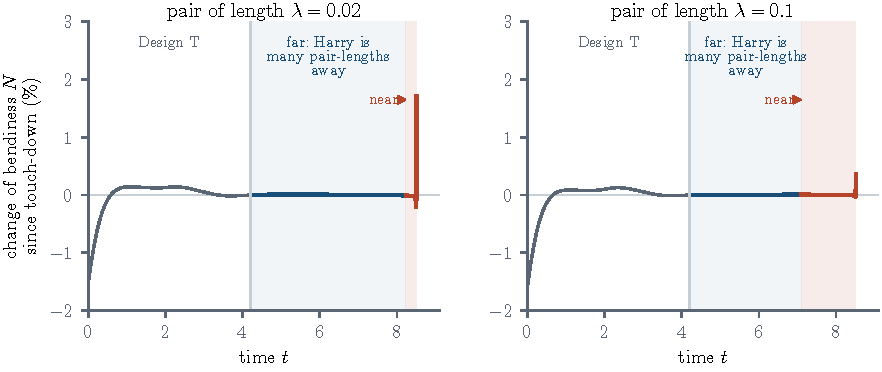
\includegraphics[width=0.95\linewidth]{figs/fig_timeline.pdf}
\caption{The life of two pairs of points on the front during a simulated walk of the kind shown in
Figure~\ref{fig:designT}, here with $v=0.1$ and $\varepsilon=0.01$ (Figure~\ref{fig:designT} itself uses
$\varepsilon=0.02$): relative change of their bendiness $N$ since touch-down. The pairs are labelled by direction; the
indicated $\lambda$ is their length in direction, and their arclength at touch-down is about $1.1\lambda$ (the far/near
test uses arclength). While the pair is far ahead of Harry (blue), $N$ hardly changes. When Harry comes within ten
pair-lengths (red), $N$ moves by at most two percent before Harry passes the pair and sees it.}
\label{fig:timeline}
\end{figure}

\textbf{Where $\varepsilon$ enters.} Only in three ways, each harmless: every pair considered has $\lambda\ge\varepsilon/2$;
$\varepsilon\le R/K_\varepsilon$; and each leg lasts at most $d_L\varepsilon$ while moving the base by at least
$\varepsilon/\kappa$, which converts time integrals into gap integrals. This is why $v_0$ and the time bound in
Theorem~\ref{thm:end} do not depend on $\varepsilon$.
}{}
\IfFileExists{main5.tex}{% main5.tex -- H-main.  Section 5: getting started -- the touch-down theorem (proved in Appendix B).
%======================================================================
\section{Getting started: the front at touch-down}\label{sec:touchdown}
%======================================================================

The end theorem needs a front that is flat on all scales between $\varepsilon$ and $R$, whose chords are not too short,
and which starts exactly at Harry. Design~T produces such a front, and the reason we can \emph{prove} it is that both of
its runs are straight. On a straight run the motion of a single candidate is completely explicit, so the front at
touch-down can be described almost in closed form, and its tangent and curvature can be followed exactly along each
run. This is what makes the starting data of the bootstrap provable.

\textbf{Two conserved quantities.} Put Harry at the origin, moving with unit velocity in the direction $1\in\C$, and
write a candidate as $r=\rho e^{i\beta}$ relative to him. Then $r'=v\hat r-1$, that is,
\[
\rho'=v-\cos\beta,\qquad \rho\beta'=\sin\beta .
\]
Two combinations are remarkably simple: $h:=\rho(\cos\beta+v)$ decreases at the constant rate $1-v^2$, and
\[
\mathcal C:=\rho\,\frg(\beta),\qquad \frg(\beta):=\frac{\sin\beta}{\tan^v(\beta/2)},
\]
is constant (check: $(\log\rho)'=(v-\cos\beta)/\rho$ and $(\log\frg(\beta))'=\frac{\cos\beta-v}{\sin\beta}\,\beta'=
(\cos\beta-v)/\rho$). So every candidate moves along an explicit curve, and its position at any time on the run is found
by solving $h(t)=h(t_1)-(1-v^2)(t-t_1)$ for $\beta$. Differentiating these formulas in the direction label $\alpha$
gives the tangent, the stretching and the curvature of the front, again exactly. Appendix~B carries this out for the two
runs of Design~T, by perturbing from $v=0$, where the front is the unit circle.

\textbf{What happens near the touch-down point.} Because run~2 is tangent to the front, the candidates on either side of
$\alpha_0$ are approached at a grazing angle. The bearing of candidate $\alpha_0\pm\xi$ from Harry has a double zero at
$\xi=0$, so these candidates come within distance about $\xi^2$ of Harry's line. Those on the forward side are still
ahead of Harry at touch-down; they form the forward arc, which starts exactly at Harry and leaves along his heading
$\hat n$. Those on the backward side were passed: the ones with $\xi^2\lesssim\varepsilon$ came within $\varepsilon$ of
Harry and are seen; the others form the tail arc, whose end lies at distance $z_0\asymp\varepsilon^{1/(2-2v)}$
(roughly $\varepsilon^{1/2}$) behind Harry, also pointing along $\hat n$ (Figure~\ref{fig:touchdown}). The rest of the
front is far from Harry and smooth; only the small hole around direction $0$, cut by run~1, needs a separate argument.

\begin{figure}[!htbp]
\centering
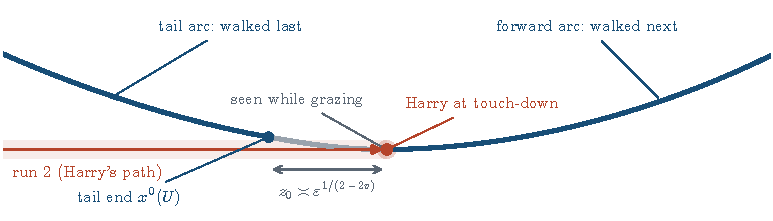
\includegraphics[width=0.92\linewidth]{figs/fig_touchdown.pdf}
\caption{The front at touch-down, seen from Harry, with his heading pointing right ($v=0.1$, $\varepsilon=0.01$,
simulated). Harry has run along a tangent to the front; the shaded band is the strip of width $2\varepsilon$ he has
searched. The forward arc starts at Harry; a sliver of length $\asymp\varepsilon^{1/(2-2v)}$ (roughly
$\varepsilon^{1/2}$) behind him has been seen while grazing; the tail end $x^0(U)$, the last point of the walk, lies at
distance $z_0\asymp\varepsilon^{1/(2-2v)}$ behind Harry and points along his path.}
\label{fig:touchdown}
\end{figure}

We now state precisely what Appendix~B proves. The front at touch-down is assembled from three kinds of labels:
virtual candidates in a window of width $\xi_1\varepsilon$ just ahead of $\alpha_0$ (they have been inside the vision disc,
and only their virtual versions are used), true candidates everywhere else, and one limit point $Z_s$ that fills the hole
left by run~1 at direction $0$. Two quantities from Appendix~B appear in the statement. The constant $\xi_1$ is chosen
so that every candidate $\alpha_0+\xi$ with $\xi\ge\xi_1\varepsilon$ stays at distance at least $2\varepsilon$ from Harry
up to $t_\td$ (Lemma~\ref{lem:B-forward}(d)); so only the window $[\alpha_0,\alpha_0+\xi_1\varepsilon)$ can contain
candidates that came within $\varepsilon$ of Harry on the forward side. The label $\be:=\alpha_0-\xie$ is the boundary
direction of the sliver seen while grazing: it is the tail direction whose minimal distance from Harry during run~2 is
exactly $\varepsilon$, i.e.\ $\mathcal C(\be)=\varepsilon\gmax$ for its run-2 integral, where $\gmax:=\max\frg$
(so $\mathcal C/\gmax$ is the minimum of $\rho=\mathcal C/\frg(\beta)$ on a run), and $\xie\asymp\varepsilon^{1/(2-2v)}$
(Lemma~\ref{lem:B-tail}(a)).

\begin{theorem}[Front at touch-down]\label{thm:touchdown}
There is an absolute $\lambda_*>0$ such that for every $\lambda_0\in(0,\lambda_*]$ there exist
$c_{\mathrm{sep}}=c_{\mathrm{sep}}(\lambda_0)>0$ and $\varepsilon_{\mathrm T}=\varepsilon_{\mathrm T}(\lambda_0)>0$
\textup(independent of $v$ and $\varepsilon$\textup), and absolute constants $v_{\mathrm T},\xi_1,G_T,\kappa_c,
C_{\mathrm{td}}>0$ \textup(independent of $\lambda_0$\textup), such that for all $v\in(0,v_{\mathrm T}]$ and
$\varepsilon\in(0,\varepsilon_{\mathrm T}(\lambda_0)]$ the following holds under Design~T, with $d=1$. First,
$t_\td=2+\sqrt3+O(v+\varepsilon)\le4$. Define $\Upsilon(\alpha)$ for
$\alpha\in[\alpha_0,2\pi+\be]$ \textup(directions taken mod $2\pi$\textup) as $x_\alpha(t_\td)$ on
$[\alpha_0,\alpha_0+\xi_1\varepsilon]$, as $S_\alpha(t_\td)$ on $[\alpha_0+\xi_1\varepsilon,2\pi+\be]\setminus\{2\pi\}$,
and as $Z_s:=\lim_{\alpha\to0^\pm}S_\alpha(t_\td)$ at $2\pi$. Its arclength reparametrisation $x^0:[0,U]\to\R^2$,
$x^0(u)=\Upsilon(\Theta(u))$, is $C^1$ with $|\partial_ux^0|\equiv1$, $|U-2\pi|\le C_{\mathrm{td}}(v+\varepsilon^{1/2})$ and $1\le U\le8$
\textup(the seen directions $(\be,\alpha_0)$, an interval of length $\xie$, are cut off\textup). Labels are arclength at
$t_\td$, quantities below are evaluated at $t_\td$, and:
\begin{itemize}
\setlength{\itemsep}{1pt}\setlength{\parskip}{0pt}
\item[\textup{(T0)}] $x^0(0)=P(t_\td)$; every $u\notin\mathcal G$ is true \textup(with direction $\Theta(u)$\textup), where
$\mathcal G$ is the set of labels with $\Theta(u)=2\pi$ or $\Theta(u)\in[\alpha_0,\alpha_0+\xi_1\varepsilon)$; for
$u\in\mathcal G$ the direction $\Theta(u)$ is seen by $t_\td$ or $u$ is true; and every $\theta\in[0,2\pi)$ is seen by
$t_\td$ or carried by a true label;
\item[\textup{(T1)}] $N(a,b)\le C_{\mathrm{td}}\lambda^{3/2-\mu_T}$ for all pairs with $\varepsilon/2\le\lambda\le\lambda_0$;
\item[\textup{(T2)}] $c(a,b)\ge\min\bigl(c_{\mathrm{sep}}(\lambda_0),\,\kappa_c(a+U-b)\bigr)$ for all pairs with $\lambda>\lambda_0$;
\item[\textup{(T3)}] $|T(u)-\hat n|\le C_{\mathrm{td}}u^{1-\mu}$ for $u\le G_T$;
\item[\textup{(T4)}] $|T(u)-\hat n|\le C_{\mathrm{td}}(U-u+z_0)^{1-\mu_T}$ for $U-u\le G_T$;
\item[\textup{(T5)}] $P(t_\td)-x^0(U)=z_0\hat n+y_0\hat n^\perp$ with $z_0\asymp\varepsilon^{1/(2-2v)}$
\textup(that is, $c\,\varepsilon^{1/(2-2v)}\le z_0\le C_{\mathrm{td}}\varepsilon^{1/(2-2v)}$ for an absolute $c>0$\textup)
and $|y_0|\le C_{\mathrm{td}}(z_0+\varepsilon)^{2-\mu_T}$.
\end{itemize}
\end{theorem}

In words: (T0) the front starts at Harry and accounts for every direction; (T1) it is flat on small scales, with a
bendiness exponent $\frac32-\mu_T$ just below the value $\frac32$ of a smooth curve; (T2) two points far apart along the
front are far apart in the plane, unless they are the two ends, which are close to each other; (T3)--(T4) both ends
leave along Harry's heading $\hat n$; (T5) the tail end is behind Harry, at a distance much larger than $\varepsilon$
but tending to zero with $\varepsilon$. Appendix~C (Lemma~\ref{lem:startchord}) turns (T1)--(T2) into the start
conditions (S1)--(S2) of Setting~(H) for the body pairs. The pairs near the tail end are the excused tail pairs of
Setting~(H); they are dealt with in the next section.

}{}
\IfFileExists{main6.tex}{% main6.tex -- H-main.  Section 6: heading, departure, assembly; proof of the main theorem.
%======================================================================
\section{Leaving the tail behind, and putting it together}\label{sec:assembly}
%======================================================================

At touch-down the last point of the walk, the tail end $x^0(U)$, sits a distance $z_0\approx\varepsilon^{1/2}$ behind
Harry. Pairs near it do not have the start data of Setting~(H) relative to the walk that is about to begin, so they are
excused until Harry's base has advanced a fixed distance $\We$. During that time two things must be shown: Harry walks
almost in a straight line, along $\hat n$ (the heading lemma), and the tail arc, which he is leaving at speed about $1$,
stays flat (the departure theorem). At the hand-over time $t_W$ the tail pairs are then far pairs with good data, and
the end theorem takes over (Figure~\ref{fig:departure}). Fix the assembly lengths
\[
\We:=\frac{c_AK_RR}{\kappa_c},\qquad \delta_0:=\frac R4,\qquad \UA:=\We+\delta_0+R,\qquad \UE:=\We+R ,
\]
and write $\frt:=t-t_\td$. All the objects needed to state the order of choices are now available.

\takeaway{The Parameter Lock}{%
\phantomsection\label{par:lock}%
After the locked numbers of Section~\ref{sec:intro}, the remaining scales are chosen in this order; no choice depends on
a later one.
\begin{enumerate}[(1)]
\setlength{\itemsep}{1pt}\setlength{\parskip}{0pt}
\item \textbf{$m=\frac1{10}$} satisfies $m^2r_*<4c_A$ with $r_*:=4$ (that is, $2m^2<1$), which the tilt chain
(Lemma~\ref{lem:tiltchain}) uses. Its smallness also makes the heading error $\omega_0$ of Lemma~\ref{lem:heading} below
at most $\frac14$: the main part of $\omega_0$ is $C_Tm(\delta_0/R)^{\gamma_D}$ with $C_T$ from
Theorem~\ref{thm:end}(c) and $\delta_0/R=\frac14$ fixed, so it does \emph{not} shrink with $R$ or $v$.
\item \textbf{$\lambda_0\in(0,\lambda_*]$ with $C_{\mathrm{td}}\lambda_0^{7/8}\le1$}, with $\lambda_*$ and
$C_{\mathrm{td}}$ from Theorem~\ref{thm:touchdown}; this fixes $c_{\mathrm{sep}}(\lambda_0)$ and
$\varepsilon_{\mathrm T}(\lambda_0)$. \textbf{Then $R>0$ small}, depending only on $m$, $\lambda_0$ and on the constants of
Theorem~\ref{thm:touchdown}: the finitely many conditions (R1)--(R5) are listed in Appendix~\ref{appC:conv}.
\item \textbf{$v_0>0$ small}, depending on $m$ and $R$, with $v_0\le\min(\frac1{23},v_{\mathrm T})$, so that every
error of size $O(v)$ or $O_R(v)$ is beaten by a fixed margin, for instance $A_0s_0=\frac14<f_F=\frac12$,
$f_F^2=\frac14<1$, $1+O_R(v)<\kappa$, and $e^{2\mu}\le\delta_1$. The explicit caps used are $\frac1{53}$, $\frac1{300}$,
$R/10$, $mR/C_1$, $3/(16C_*)$ and $R/(2\cdot10^4)$ (Appendices~A and~C).
\item \textbf{$\varepsilon_*>0$ small}, depending on $\lambda_0$ and $R$ only:
$\varepsilon_*\le\min(\varepsilon_{\mathrm T}(\lambda_0),R/K_\varepsilon)$, $C_{\mathrm{td}}\varepsilon_*^{1/2}\le R$,
and so small that the tail end at touch-down is at distance at least $2\varepsilon$ behind Harry (possible uniformly in
$v\le\frac1{23}$, since that distance is of order $\varepsilon^{1/(2-2v)}\gg\varepsilon$).
\end{enumerate}}

Two different flatness exponents are used: the walk as a whole is controlled with $\gamma=\frac23$, its first stretch
(the Stage-A chase below) with $\gamma_D=\frac34$. The reason is the hand-over at $t_W$: the departure theorem loses a
factor $(R/\lambda)^{\nu_D}$ with $\nu_D=O(v)$ (Theorem~\ref{thm:departure}(iv)), and the tail data (TW) for the walk need
$\gamma+\nu+\nu_D\le\gamma_D$, so the walk must use a smaller exponent than the departure and heading estimates.

\begin{figure}[!htbp]
\centering
\begin{tikzpicture}[scale=1.25,>=Stealth]
  \draw[muted,dashed] (-3.8,0) -- (4.6,0) node[right,font=\small] {$\hat n$};
  \draw[accent,very thick,->] (0,0) -- (2.4,0.18);
  \fill[black] (0,0) circle (1.8pt) node[below=2pt,font=\small] {$P(t_\td)$};
  \fill[accent] (2.4,0.18) circle (2pt);
  \node[accent,font=\small,align=center] at (2.75,-0.5) {Harry at time $t$, heading\\[-1pt]within $h_H(\frt)$ of $\hat n$};
  \draw[primary,very thick] (2.6,0.2) .. controls (3.2,0.26) and (3.8,0.34) .. (4.5,0.48);
  \node[primary,font=\footnotesize] at (3.7,0.7) {front ahead};
  \draw[primary,very thick] (-0.95,-0.08) .. controls (-1.9,-0.16) and (-2.8,-0.32) .. (-3.6,-0.58);
  \fill[primary] (-0.95,-0.08) circle (2pt) node[above left=1pt,font=\small] {$x^0(U)$};
  \draw[<->,muted] (-0.95,0.25) -- (0,0.25) node[midway,above,font=\footnotesize] {$z_0\approx\varepsilon^{1/2}$};
  \node[font=\footnotesize,primary] at (-2.4,-0.75) {tail arc (length $\UE$)};
  \draw[<->,muted] (-2.3,0.9) -- (2.4,0.9) node[midway,above,font=\footnotesize]
     {distance grows at rate $\ge\frac12$: $\rho_s\ge\frac12(s+z_0+\frt)$};
\end{tikzpicture}
\caption{Leaving the tail behind. While Harry walks the first stretch of the front, his heading stays close to the
touch-down heading $\hat n$, so he moves away from the tail arc at speed about $1$. The tail arc stays flat, and by
the time Harry has walked a distance $\We$ its pairs are far from him and satisfy the start data of the end theorem.}
\label{fig:departure}
\end{figure}

\textbf{The heading.} To control Harry's direction during the first stretch we apply the end theorem to a short initial
piece of the front: the \emph{Stage-A chase} is Design~T followed by the greedy chase on the working front
$x^0|_{[0,\UA]}$ (so $U=\UA$ and the cut is $b_c=\UA$ in Setting~(H)), with exponent $\gamma_D=\frac34$ and excuse
length $0$. Stage~A is a bookkeeping device: its legs coincide with those of the real walk as long as the base is below
$\We$ (causality), so the path is the same and only the cut differs. On this piece the end theorem gives tilt bounds;
near the start of the walk the front is aligned with $\hat n$ by (T3).

\begin{lemma}[Heading of the first legs]\label{lem:heading}
Let $R$, $v_0$ and $\varepsilon_*$ be chosen as in the Parameter Lock, $v\le v_0$, $\varepsilon\le\varepsilon_*$, and
suppose the Stage-A chase satisfies the conclusions of Theorem~\ref{thm:end} with exponent $\gamma_D$ and excuse length
$0$. There are constants $C_H=C_H(R)$ and $\omega_0\le\frac14$, independent of $v$ and $\varepsilon$, such that for every
non-final leg $j+1$ of the Stage-A chase with $a_j<\We$ and every $t$ in that leg,
\[
|\hat u_{j+1}-\hat n|\le h_H(\frt):=\min\bigl(C_H(\frt+\varepsilon)^{\gamma_D},\,\omega_0\bigr).
\]
\end{lemma}

Here $\omega_0=C_Tm(\delta_0/R)^{\gamma_D}+O(R^{7/8})+O(v_0)$, with first term about $0.197$ (Parameter Lock, item
(1)). The two branches of $h_H$ are both needed: the cap $\omega_0$ keeps Harry moving away from the tail, and the branch
$C_H(\frt+\varepsilon)^{\gamma_D}$ makes the integral $\int h_H^2\,d\frt/(\frt+\varepsilon)$ bounded independently of
$\varepsilon$.

\begin{theorem}[Departure]\label{thm:departure}
Let $x(s,t)$, $s\in[0,\UE]$, be a virtual flow of $P$ from a curve $x^\circ$ with $|\partial_sx^\circ|\equiv1$, started
at $t_\td$. Let $\hat u$ be a unit vector, $D>0$, and write $r_s=x_s-P=z_s\hat u+y_s\hat u^\perp$ and
$X_s(\frt):=s+z_0+\frt$ for $\frt\in[0,D]$. Let $C_D\ge1$, $C_H>0$, $0<\omega_0\le\frac14$, and
$h_H(\frt):=\min(C_H(\frt+\varepsilon)^{\gamma_D},\omega_0)$. Assume:
\begin{itemize}
\setlength{\itemsep}{1pt}\setlength{\parskip}{0pt}
\item[\textup{(D0)}] $x(0,t_\td)-P(t_\td)=z_0\hat u+y_0\hat u^\perp$ with $z_0\ge2\varepsilon$ and $|y_0|\le C_Dz_0^{1+\gamma_D}$;
\item[\textup{(D1)}] $|T(s,t_\td)-\hat u|\le C_D(s+z_0)^{\gamma_D}$ for $s\in[0,\UE]$;
\item[\textup{(D2)}] $|P'|=1$, $P'\cdot\hat u<0$ and $|\hat u\times P'|\le h_H(\frt)$ for a.e.\ $\frt\in[0,D]$;
\item[\textup{(D3)}] $8C_D(\UE+z_0+D)^{\gamma_D}\le1$ \textup(the departure window is small; in particular
$D+\varepsilon\le1$, as $z_0\ge2\varepsilon$\textup).
\end{itemize}
Then, for $v\le v_0$ with $v_0$ small depending only on $C_D,C_H,\omega_0$, and with $\nu_D:=2\mathcal A^*(4)v$
\textup($\mathcal A^*$ from Lemma~\ref{lem:duhamel}\textup) and $k_D:=10$, for all $s\in[0,\UE]$ and $\frt\in[0,D]$:
\begin{enumerate}[(i)]
\setlength{\itemsep}{1pt}\setlength{\parskip}{0pt}
\item $z_s\ge\frac12X_s(\frt)$, hence $\rho_s\ge\frac12X_s(\frt)\ge\varepsilon$;
\item $|y_s(\frt)|\le CX_s(\frt)\bigl(X_s(0)^{\gamma_D}+h_H(\frt)\bigr)$ and $|T(s,t)-\hat u|\le CX_s(\frt)^{\gamma_D}$;
\item $1\le w\le1+O_R(v)$, so $\lambda\le l_t(a,b)\le(1+O_R(v))\lambda$ for every pair;
\item for every pair $(a,b)\subset[0,\UE]$ with $\lambda\ge\varepsilon/2$,
\[
N(a,b;t)\le\Bigl(1+\frac{\frt}{k_D\lambda}\Bigr)^{\nu_D}\Bigl[N(a,b;t_\td)+O_R(v)\,\lambda^{1/2+\gamma_D}\Bigr].
\]
\end{enumerate}
Here $C$ and the implied constants in $O_R(v)$ depend only on $C_D$, $C_H$ and $\omega_0$; none depends on $\varepsilon$.
\end{theorem}

The mechanism is simple. Harry's velocity points away from the tail up to an angle of at most $\arcsin\frac14$, so every
point of the tail arc falls behind at rate at least $\frac12$, which gives (i); then the arc feels only the smooth far
field $x/|x|$, which can turn its tangent by an amount $\int v\,dt/\rho\approx v\log$, and (ii)--(iv) follow from the
variation-of-constants formula and the Duhamel inequality. Both proofs are in Appendix~C.

\begin{proposition}[Conditional form for $d=1$]\label{prop:cond}
Let $v_0,\varepsilon_*>0$ be chosen by the Parameter Lock. For every $v\in(0,v_0]$ and $\varepsilon\in(0,\varepsilon_*]$,
Design~T followed by the greedy chase on $x^0$ cut at $U$ is well defined, $1$-Lipschitz, depends only on
$(v,\varepsilon)$, and sees every $\alpha\in[0,2\pi)$ by time $T_\stopp\le t_\td+\kappa U/(1-v)\le15$.
\end{proposition}

The proof is in Appendix~C; Table~\ref{tab:coverage} records which result controls which pairs at which times (the
tail arc is read backwards from $x^0(U)$, with $\hat u:=-\hat n$, when Theorem~\ref{thm:departure} is applied).

\begin{table}[!htbp]
\centering
\small
\begin{tabularx}{\linewidth}{l l >{\raggedright\arraybackslash}X}
\toprule
\textbf{What} & \textbf{When} & \textbf{Controlled by} \\
\midrule
Directions seen on runs 1--2, hole, grazing sliver & $[0,t_\td]$ & Theorem~\ref{thm:touchdown} (T0) \\
Stage-A chase on $[0,\UA]$ ($\gamma_D=\frac34$) & $[t_\td,t_W]$ & Theorem~\ref{thm:end} (excuse length $0$) \\
Harry's heading, $|P'-\hat n|\le h_H$ & $[t_\td,t_W]$ & Lemma~\ref{lem:heading} \\
Tail arc $\{U-u\le\UE\}$; tail data (TW) & $[t_\td,t_W]$; at $t_W$ & Theorem~\ref{thm:departure} \\
Body pairs of $[0,U]$ ($\gamma=\frac23$) & $[t_\td,T_\stopp]$ & Theorem~\ref{thm:end} with (S1)--(S2) \\
Tail pairs of $[0,U]$ ($\gamma=\frac23$) & $[t_W,T_\stopp]$ & Theorem~\ref{thm:end} with (TW) \\
All true labels seen & by $T_\stopp\le15$ & Theorem~\ref{thm:end}(b) \\
\bottomrule
\end{tabularx}
\caption{Every direction, every pair and every time interval is covered by one of the results.}
\label{tab:coverage}
\end{table}

\begin{proof}[Proof of Theorem~\ref{thm:main}]
Let $v_0,\varepsilon_*$ be as in Proposition~\ref{prop:cond} and $T_0:=15$. Given $d>0$, $\varepsilon\in(0,d)$ and
$v\in(0,v_0]$, put $\hat\varepsilon:=\min(\varepsilon/d,\varepsilon_*)$, let $P$ be the path of
Proposition~\ref{prop:cond} for $(v,\hat\varepsilon)$, and set $H(t):=dP(t/d)$. Then $H(0)=0$ and $|H'|\le1$ a.e. If
$S^P_\alpha$ denotes the candidate for $P$ starting at $e^{i\alpha}$, then $t\mapsto dS^P_\alpha(t/d)$ solves
\eqref{eq:snitch} for $H$ with start $de^{i\alpha}$, so by uniqueness $S_\alpha(t)=dS^P_\alpha(t/d)$ on the interval of
existence. Proposition~\ref{prop:cond} gives $t'\le15$ with $|S^P_\alpha(t')-P(t')|\le\hat\varepsilon$; hence
$|S_\alpha(dt')-H(dt')|\le d\hat\varepsilon\le\varepsilon$ with $dt'\le T_0d$. Finally, $d\hat\varepsilon=\varepsilon'$,
so $H$ is exactly the path described in the theorem.
\end{proof}



}{}
\IfFileExists{main7.tex}{% main7.tex -- H-main.  Section 7: from eps > 0 to exact capture.
%======================================================================
\section{From $\varepsilon>0$ to exact capture}\label{sec:exact}
%======================================================================

Theorem~\ref{thm:main} gives, for every vision radius $\varepsilon$, a path that sees every direction by the same time
$T_0d$. All these paths are $1$-Lipschitz on the common interval $[0,T_0d]$, so a subsequence converges uniformly as
$\varepsilon\to0$ (Figure~\ref{fig:limit}). If the limit path missed some direction, that candidate would stay a positive
distance away from it; by continuity it would also stay away from the nearby paths with tiny $\varepsilon$, which is
impossible. This is why the uniformity of the time bound in $\varepsilon$ is the crux of the whole paper: if the search
time grew as $\varepsilon\to0$, there would be no common interval and no limit.

\begin{figure}[!htbp]
\centering
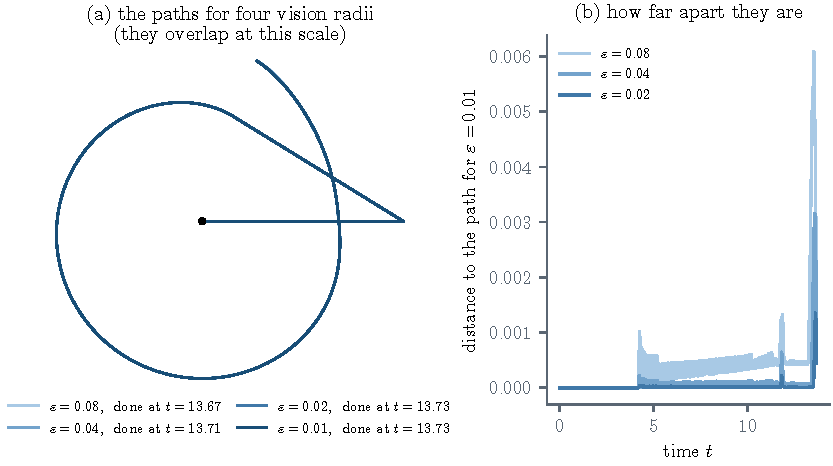
\includegraphics[width=0.95\linewidth]{figs/fig_limit.pdf}
\caption{The paths of the proof for four vision radii ($v=0.1$, simulated). (a) They are indistinguishable at this
scale, and all finish at about the same time. (b) Their distance from the path for $\varepsilon=0.01$; it shrinks
with $\varepsilon$, except for spikes near the end of the walk, which come from different final legs. The exact catch of Corollary~\ref{cor:exact} comes from a limit of such paths.}
\label{fig:limit}
\end{figure}

\begin{lemma}[Compactness]\label{lem:compact}
Let $d>0$, let $D_1\subset D_2\subset\cdots$ be finite sets of directions whose union is dense in $[0,2\pi)$, and let
$\varepsilon_N\to0$. Suppose that for each $N$ a $1$-Lipschitz path $H_N$ with $H_N(0)=0$ comes within $\varepsilon_N$ of
every candidate $S_\alpha$, $\alpha\in D_N$ \textup(the candidates for the path $H_N$\textup), by a time $\bar T$
independent of $N$. Then there is a $1$-Lipschitz path $H$ with $H(0)=0$ that catches every direction by time $\bar T$.
\end{lemma}

\begin{proof}
By the Arzel\`a--Ascoli theorem a subsequence, still written $H_N$, converges uniformly on $[0,\bar T]$ to a
$1$-Lipschitz path $H$ with $H(0)=0$. For a $1$-Lipschitz path $G$ write $\rho^G_\alpha:=|S_\alpha-G|$, where $S_\alpha$ is
the candidate $\alpha$ for the path $G$; it is defined until the catch, and $|(\rho^G_\alpha)'|\le1+v$. We use the
elementary inequality $|y/|y|-z/|z||\le2|y-z|/\max(|y|,|z|)$.

\emph{Claim.} Let $G,G_k$ be $1$-Lipschitz paths on $[0,\bar T]$ with $\|G_k-G\|_\infty\to0$, and suppose
$\rho^G_\alpha\ge c>0$ on $[0,\tau]$, $\tau\le\bar T$. Put $\tau':=\min(\tau+c/(2(1+v)),\bar T)$. Then there are a
neighbourhood $\mathcal U$ of $\alpha$ and a $k_0$ such that for $\alpha'\in\mathcal U$ and $k\ge k_0$ the candidate
$\alpha'$ for $G_k$ is defined on $[0,\tau']$ and $\rho^{G_k}_{\alpha'}\ge c/4$ there.

Indeed, since $|(\rho^G_\alpha)'|\le1+v$, the candidate $S:=S_\alpha$ for $G$ is defined on $[0,\tau']$ with
$\rho^G_\alpha\ge c/2$ there. Let $\tilde S:=S_{\alpha'}$ be the candidate for $G_k$. As long as
$|S-G|,|\tilde S-G_k|\ge c/4$, the inequality above gives
$|\tilde S-S|(t)\le|\tilde S-S|(0)+(8v/c)\int_0^t\bigl(|\tilde S-S|+\|G_k-G\|_\infty\bigr)$, so by Gr\"onwall's
inequality $|\tilde S-S|\le b_k:=\bigl(|e^{i\alpha'}-e^{i\alpha}|d+(8v/c)\bar T\|G_k-G\|_\infty\bigr)e^{8v\bar T/c}$.
Choose $\mathcal U$ and $k_0$ with $b_k+\|G_k-G\|_\infty<c/4$. Let $I$ be the set of $s\in[0,\tau']$ such that $\tilde S$
is defined on $[0,s]$ with $|\tilde S-G_k|\ge c/4$ there. Then $0\in I$ (as $|\tilde S(0)-G_k(0)|=d\ge c$), $I$ is
closed (as $|\tilde S'|=v$, $\tilde S$ extends continuously to $\sup I$, where $|\tilde S-G_k|\ge c/4>0$ still holds,
so it is defined there), and for $s\in I$ the bound gives $|\tilde S-G_k|\ge|S-G|-b_k-\|G_k-G\|_\infty>c/4$ on $[0,s]$, so $I$ also
contains a neighbourhood of $s$ in $[0,\tau']$. Hence $I=[0,\tau']$, proving the claim.

Now fix $\alpha\in D_M$. For $N\ge M$ we have $\alpha\in D_N$; let $t_N\le\bar T$ be the first time with
$\rho^{H_N}_\alpha(t_N)\le\varepsilon_N$, and pass to a subsequence with $t_N\to t^*\le\bar T$. If $H$ did not catch
$\alpha$ by time $t^*$, then $\rho^H_\alpha$ would be defined and positive on $[0,t^*]$, hence $\ge c>0$ there, and
the claim (with $G=H$, $G_k=H_N$, $\alpha'=\alpha$, $\tau=t^*$) would give $\rho^{H_N}_\alpha\ge c/4$ on
$[0,\min(t^*+c/(2(1+v)),\bar T)]$, an interval containing $t_N$ for large $N$; this contradicts $\varepsilon_N\to0$.
So $H$ catches every direction of $\bigcup_ND_N$ by time $\bar T$. Finally, the claim with $G_k=G=H$ and $\tau=\bar T$
shows that the set of directions \emph{not} caught by $H$ on $[0,\bar T]$ is open. It is disjoint from the dense set
$\bigcup_ND_N$, hence empty.
\end{proof}

\begin{proof}[Proof of Corollary~\ref{cor:exact}]
By scaling we may take $d=1$. Fix $v\in(0,v_0]$ and apply Lemma~\ref{lem:compact} with $\bar T:=T_0$,
$D_N:=\{2\pi i/2^N:0\le i<2^N\}$, $\varepsilon_N:=2^{-N}\varepsilon_*$, and $H_N$ the path of Theorem~\ref{thm:main}
for $(v,\varepsilon_N,1)$. Theorem~\ref{thm:main} says exactly that $H_N$ comes within $\varepsilon_N$ of every candidate
by time $T_0$, so the lemma gives a single path that catches every direction by time $T_0$.
\end{proof}

\textbf{What the proof does not give.} The argument is qualitative in $v$: it shows that \emph{some} $v_0>0$ works, and
the companion paper \cite{short} shows that $v_0=5.8\cdot10^{-3}$ does, with explicit constants checked by computer. The
simulations suggest that Design~T followed by the walk succeeds for much larger $v$, but we have no estimate of how
large $v$ may be for the method itself. The limit path of Corollary~\ref{cor:exact} is not explicit.
}{}

\begin{thebibliography}{9}
\bibitem{HLP}
G.~H.~Hardy, J.~E.~Littlewood, and G.~P\'olya,
\emph{Inequalities}, 2nd ed., Cambridge University Press, Cambridge, 1952.
\bibitem{Hartman}
P.~Hartman,
\emph{Ordinary Differential Equations}, 2nd ed., Classics in Applied Mathematics~38, SIAM, Philadelphia, 2002.
\bibitem{short}
\emph{A path fixed in advance that finds a slow fleeing point} (the companion paper with explicit constants,
$v_0=5.8\cdot10^{-3}$, $T_0=13.1$; file \texttt{short/snitch.pdf}).
\end{thebibliography}

\appendix
\IfFileExists{appA.tex}{% appA.tex -- writer H-walk.  Appendix A: walking the front (proof of the End Theorem).
% Uses the labels of the main text: thm:end, def:chase, lem:F, lem:vflow, lem:seen, lem:chords, lem:excess,
% lem:splittilt, lem:Eprime, lem:duhamel (streamlined labels).  Defines: app:walk, lem:chase, lem:toolkit,
% lem:locality, lem:tiltchain, lem:cont, prop:far, prop:near, prop:length, eq:Emu, eq:Imp.
\providecommand{\eps}{\varepsilon}
\providecommand{\Fam}{\mathcal{F}}
\providecommand{\FamS}{\mathcal{F}_*}
\providecommand{\rhoarc}{\underline{\rho}}
\providecommand{\Tdef}{T_{\mathrm{def}}}

\section{Walking the front: proof of the End Theorem}\label{app:walk}

This appendix proves Theorem~\ref{thm:end}, along the plan sketched after its statement: a continuity argument
(Lemma~\ref{lem:cont}) reduces it to the three estimates of Propositions~\ref{prop:far}, \ref{prop:near} and
\ref{prop:length}; Sections~\ref{app:walk:chase}--\ref{app:walk:tools} collect the bookkeeping these estimates use.

\subsection{Conventions}\label{app:walk:conv}

\textbf{Parameters.} We use the locked numbers of Section~\ref{sec:intro} (in particular $\delta_1=\frac54$),
$U\le U_0=8$, and $\gamma\in\{\frac23,\frac34\}$ (the main
chase uses $\gamma=\frac23$, Stage~A uses $\gamma=\gamma_D=\frac34$; everything below holds for both). As in
Setting~(H), $M=mR^{-\gamma}$ (so $M\lambda^\gamma=m(\lambda/R)^\gamma\le m$ for $\lambda\le R$),
$\eps\le R/K_\eps$, and we assume $R\le1$. The derived constants are
\[
c_6:=\frac{1+\delta_1}{c_A}=\frac92,\qquad
c_\rho^*:=c_A-\frac{2\delta_1}{K_f}=\frac14,\qquad
c_R^*:=c_AK_R-\frac{\delta_1}{K_\eps}=\frac{47}8,\qquad
\chi_g:=\kappa d_L=\frac52,
\]
\[
C_T:=\frac{\sqrt5\,(1-2m^2)^{-1/2}}{1-2^{-\gamma}}\ \ \bigl(<6.11\text{ for }\gamma=\tfrac23,\ <5.58\text{ for }\gamma=\tfrac34\bigr),
\qquad C_\mu:=1+\kappa C_T^2<48 .
\]
Note $c_\rho^*K_f=\frac52\ge2$; this is the inequality needed in Step~1 of the proof of Proposition~\ref{prop:far}.

\textbf{What ``$C$'' means.} A letter $C$ (possibly with an index) is a positive number computed from the locked
parameters only ($m=\frac1{10}$ included). It never depends on $\eps$, $v$, $R$, $\lambda$, $t$, $U$ or on the front;
where $R$ enters, it is written out as a power of $R$. The vision radius enters only in the three ways listed at the
end of Section~\ref{sec:chase} (the third is Lemma~\ref{lem:toolkit}(b) below).

\textbf{How small $v_0$ is.} Always $v\le v_0\le\frac1{10}$. Then, with $\mu=v/(1-v)\le\frac19$,
\begin{equation}\label{eq:V0}
\tfrac1{1-v}\le\tfrac{10}9\le d_L,\qquad e^{2\mu}\le e^{2/9}<1.25=\delta_1 .
\end{equation}
Propositions~\ref{prop:far}--\ref{prop:length} add finitely many conditions $v_0\le R/C$; so $v_0=v_0(m,R)$, as in
Theorem~\ref{thm:end}. Of the number $\delta_t=O_R(v)$ of Setting~(H) we only use $\delta_t\le\frac1{16}$ (true once
$v_0$ is small).

\subsection{The chase}\label{app:walk:chase}

During a leg the pursuer runs straight at a point of the front, and that point flees straight away from it; in the
short time $\eps/(1-v)$ that a leg lasts, the front can stretch only by the factor $e^{2\mu}\approx1$.

\begin{lemma}[Chase basics]\label{lem:chase}
Assume the proviso holds at every non-final leg start that is reached. Then:
\begin{enumerate}
\setlength{\itemsep}{1pt}\setlength{\parskip}{0pt}
\item[(0)] either the chase stops, or $t_j\to\infty$; and $P$ is $1$-Lipschitz;
\item[(1)] during leg $j+1$ the points $x_{a_j},P,x_{a_{j+1}}$ lie on a line in this order, $|x_{a_{j+1}}-P|$
decreases at rate at least $1-v$, and the leg lasts at most $c(a_j,a_{j+1};t_j)/(1-v)\le d_L\eps$;
\item[(2)] every true label $u\in[a_j,a_{j+1}]$ is seen by time $t_j$ (this includes the final leg);
\item[(3)] during leg $j+1$: $l_t(a,b)\le\delta_1l_{t_j}(a,b)$ for all $a<b$, and $|P-x_{a_j}|\le\delta_1\eps$;
\item[(4)] if a path $\tilde P$ equals $P$ on $[0,t_j]$, the working fronts of $P$ and $\tilde P$ agree on $[t_\td,t_j]$.
\end{enumerate}
\end{lemma}

\begin{proof}
By Lemma~\ref{lem:vflow}(a) and $A\le a^*I\le(2/\eps)I$ (Lemma~\ref{lem:F}(ii)), $w_t\le(2v/\eps)w$; hence
$l'\le(2v/\eps)l$ for every pair.

(1) Let $\rho$ solve $\rho'=-1+vf(\rho)$ with $\rho(t_j)=c(a_j,a_{j+1};t_j)>0$. Since $F(\rho\hat u)=f(\rho)\hat u$,
the point $y:=P+\rho\hat u_{j+1}$ solves $y'=vF(y-P)$ with $y(t_j)=x_{a_{j+1}}(t_j)$, so $y=x_{a_{j+1}}$ by uniqueness
while $\rho>0$; and $\rho'\le-(1-v)$ because $f\le1$. Likewise $P-\sigma\hat u_{j+1}$, with $\sigma'=1+vf(\sigma)$,
$\sigma(t_j)=0$, solves the equation of $x_{a_j}$ (as $F(-\sigma\hat u)=-f(\sigma)\hat u$), and $\sigma\ge0$. Finally
$c(a_j,a_{j+1};t_j)\le l_{t_j}(a_j,a_{j+1})\le\eps$ and $1/(1-v)\le d_L$ by \eqref{eq:V0}.

(3) Lengths grow at most by the factor $\exp\bigl((2v/\eps)\cdot\eps/(1-v)\bigr)=e^{2\mu}\le\delta_1$ during the leg.
By (1), $|P-x_{a_j}|=\sigma\le c(a_j,a_{j+1};t)\le l_t(a_j,a_{j+1})\le\delta_1\eps$.
(0) On $[t_\td,T]$, $w\le e^{2v(T-t_\td)/\eps}$; a non-final leg has $l_{t_j}(a_j,a_{j+1})=\eps$ (maximality and
continuity of $l$ in the label), so it moves the base by at least $\eps e^{-2v(T-t_\td)/\eps}$, and only finitely many
legs start before $T$. $P$ is piecewise linear with speed $\le1$.
(2) At $t_j$, $P=x_{a_j}$, so $\rho_u(t_j)=c(a_j,u;t_j)\le l_{t_j}(a_j,u)\le\eps$ by the choice of $a_{j+1}$; apply
Lemma~\ref{lem:seen}. (4) The front at time $t$ depends only on $x^0$ and on $P$ on $[t_\td,t]$ (uniqueness).
\end{proof}

\subsection{The toolkit}\label{app:walk:tools}

\textbf{Reminders from Setting (H).} The base at time $t$ is $a_{j(t)}$, where $j(t)=j$ for $t\in(t_j,t_{j+1}]$ and
$j(t_0)=0$. A leg start $t_j$ ($j\ge1$) belongs to both legs $j$ and $j+1$: a statement about leg $j+1$ may be applied
at $t_j$ with the base $a_j$, since $P(t_j)=x_{a_j}(t_j)$. For a tail pair, $t_W$ is treated as a point of leg
$j_W+1$ (base $a_{j_W}$). \emph{Every pair with $\lambda\le R$ is good}: a pair that is not good has $a<\We$ and
$U-b<\We$, hence $\lambda>U-2\We\ge R+\eps$. Families shrink in time (a pair of the family of leg $k+1$, $k>j$, has
$a\ge a_k\ge a_{j+1}$), and the gap of a fixed label is non-increasing in $t$ and constant on each leg. $\Tdef\le\infty$
is the supremum of the times up to which the chase is defined.

\begin{lemma}[Toolkit]\label{lem:toolkit}
\textup{(CA)} For every good pair with $\lambda\ge\eps/2$ and every $t\ge t_\td$: $c(a,b;t)\ge c_A\min(\lambda,K_RR)$.
In particular $c(a,b;t)\ge c_A\lambda$ for every pair with $\eps/2\le\lambda\le R$.

\textup{(c) (Distance from the base.)} Let $t$ lie in leg $j+1$ and let $s\ge a_j$ be a label with $U-s\ge\We$ or
$a_j\ge\We$. Then
\[
\rho_s(t)\ge c_A\min(s-a_j,K_RR)-\delta_1\eps,\qquad \max(\rho_s(t),\eps)\ge\min(s-a_j,K_RR)/c_6 .
\]
Now let $t'\le\Tdef$ and assume that \textup{(J1)} holds at every leg start $t_i\le t'$ for all pairs of $\FamS(t_i)$.
\begin{enumerate}
\setlength{\itemsep}{1pt}\setlength{\parskip}{0pt}
\item[\textup{(a)}] \emph{(Legs.)} Let $t_j\le t'$ be a leg start. (a1) If $U-a_j\ge\eps/2$ and leg $j+1$ is not final,
then $a_{j+1}-a_j\in[\eps/\kappa,\eps]$ and $l_{t_j}(a_j,a_{j+1})=\eps$. (a2) If $U-a_j<\eps/2$, leg $j+1$ is final; if
$a_j<\We$, it is not final. (a3) If leg $j+1$ is not final, $c(a_j,a_{j+1};t_j)\ge c_A(a_{j+1}-a_j)>0$: the proviso
holds. (a4) At most $\kappa U/\eps$ non-final legs start in $[t_\td,t']$, each lasts at most $d_L\eps$, and
$t'-t_\td\le\chi_gU\le20$.
\item[\textup{(b)}] \emph{(Gap--time integrals.)} Fix a label $a$ and a set $\mathcal T\subset[t_\td,t']$ of times at
which $g(\tau):=a-a_{j(\tau)}\ge0$. The values of $g$ on distinct legs differ by at least $\eps/\kappa$, and:
(i) if $g_{\min}$ is the smallest value of $g$ on $\mathcal T$ and $h\ge0$ is non-increasing on $[g_{\min},\infty)$,
then $\int_{\mathcal T}h(g(\tau))\,d\tau\le d_L\eps\,h(g_{\min})+\chi_g\int_{g_{\min}}^\infty h(y)\,dy$;
(ii) if $g\le\bar g$ on $\mathcal T$ and $h\ge0$ is non-decreasing on $[0,\bar g+\eps/\kappa]$, then
$\int_{\mathcal T}h(g(\tau))\,d\tau\le\chi_g\int_0^{\bar g+\eps/\kappa}h(y)\,dy$;
(iii) at most $\kappa x/\eps+1$ legs meet $\{\tau\in\mathcal T:g(\tau)\le x\}$.
\end{enumerate}
\end{lemma}

The point of (b): a leg lasts about $\eps$ and the gap drops by about $\eps$ per leg, so ``time at gap $g$'' is
comparable to ``$dg$''.

\begin{proof}
(CA) Chords are non-decreasing in time (Lemma~\ref{lem:chords}(a)); apply (S1). Pairs with $\eps/2\le\lambda\le R$ are
good, and $R\le K_RR$.

(c) Put $\Delta:=s-a_j$ and $y:=\min(\Delta,K_RR)$. If $\Delta<\eps/2$, the first right-hand side is negative and the second is
$<\eps$. Otherwise $(a_j,s)$ is good, and by (CA) and Lemma~\ref{lem:chase}(3),
$\rho_s\ge|x_s-x_{a_j}|-|P-x_{a_j}|\ge c_Ay-\delta_1\eps$. If $c_Ay-\delta_1\eps\ge y/c_6$ we are done; otherwise,
since $c_A-1/c_6=c_A\delta_1/(1+\delta_1)$, we get $y<(1+\delta_1)\eps/c_A=c_6\eps$, so $\max(\rho_s,\eps)\ge\eps>y/c_6$.

(a) Always $a_{j+1}-a_j\le l_{t_j}(a_j,a_{j+1})\le\eps$, since $w\ge1$. The pairs $(a_j,s)$, $\eps/2\le s-a_j\le\eps$,
lie in $\Fam(t_j)$ and are admissible (if $t_j<t_W$, then $a_j<\We$ and $U-s\ge U-\We-\eps\ge\We$), so (J1) applies.
(a1) The label $s:=a_j+\eps/2\le U$ has $l_{t_j}(a_j,s)\le\kappa\eps/2<\eps$, so $a_{j+1}\ge s$. If the leg is not
final, $l_{t_j}(a_j,a_{j+1})=\eps$ by maximality, and (J1) for $(a_j,a_{j+1})$ gives $\eps\le\kappa(a_{j+1}-a_j)$.
(a2) A final leg has $U-a_j\le l_{t_j}(a_j,U)\le\eps$, so $a_j\ge U-\eps>\We$ if $\We>0$; thus legs with $a_j<\We$ are
not final. Now let $U-a_j<\eps/2$ (so $a_j\ge\We$ and $t_j\ge t_W$); we argue by induction on $j$. For $j=0$,
$l_{t_0}(0,U)=U<\eps/2$. For $j\ge1$, leg $j$ was walked, so by induction $U-a_{j-1}\ge\eps/2$ and by (a1)
$\lambda_1:=a_j-a_{j-1}\in[\eps/\kappa,\eps]$ with $l_{t_{j-1}}(a_{j-1},a_j)=\eps$. The pair $(a_{j-1},U)$ has length
$\lambda_1+(U-a_j)\in[\eps/2,\frac32\eps]\subset[\eps/2,R]$ and lies in $\Fam(t_j)=\FamS(t_j)$, so by (J1) and the
monotonicity of lengths in $t$,
$l_{t_j}(a_j,U)\le\kappa\cdot\frac32\eps-\eps=\frac78\eps<\eps$, i.e.\ $a_{j+1}=U$. (Here $\kappa<\frac43$ is used.)
(a3) By (a1),(a2), $\eps/2\le a_{j+1}-a_j\le\eps\le R$; apply (CA).
(a4) Each non-final leg moves the base by at least $\eps/\kappa$ (by (a1),(a2)) and the moves add up to at most $U$; each
lasts at most $d_L\eps$ by Lemma~\ref{lem:chase}(1). Hence $t'-t_\td\le(\kappa U/\eps)d_L\eps=\chi_gU\le\frac52\cdot8$.

(b) Non-final legs move the base by at least $\eps/\kappa$ (part (a)), so the values of $g$ are spaced by
$\eps/\kappa$; the final leg occupies no time. (i) Let $g_1>\dots>g_n=g_{\min}$ be the values. For $i<n$,
$g_i-\eps/\kappa\ge g_{i+1}\ge g_{\min}$ and $h$ is non-increasing, so $h(g_i)\le(\kappa/\eps)\int_{g_i-\eps/\kappa}^{g_i}h$;
these intervals are disjoint. Each leg lasts at most $d_L\eps$, so the integral is at most
$d_L\eps\,h(g_{\min})+d_L\eps(\kappa/\eps)\int_{g_{\min}}^\infty h$. (ii) Likewise
$h(g_i)\le(\kappa/\eps)\int_{g_i}^{g_i+\eps/\kappa}h$ for every value, with disjoint intervals in
$[0,\bar g+\eps/\kappa]$. (iii) The values in $[0,x]$ are spaced by $\eps/\kappa$.
\end{proof}

\textbf{Start times and bases.} For a pair $(a,b)\in\FamS(t)$ its \emph{start time} is $t_\circ:=t_\td$ if it is a body
pair and $t_\circ:=t_W$ if it is a tail pair; at its start time a pair satisfies (S2) resp.\ (TW). For
$\tau\in[t_\circ,t]$ let $\bar a(\tau):=a_{j(\tau)}$ and $\bar a^+(\tau):=a_{j(\tau)+1}$ be the base and the next base,
with the convention $\bar a(t_W):=a_{j_W}$, $\bar a^+(t_W):=a_{j_W+1}$ for tail pairs.

The next lemma says that the bootstrap bounds may be used, at all times since the start time, on the pair itself and
on the pairs lying between the pursuer and it; the only subtlety is the excused tail.

\begin{lemma}[Locality]\label{lem:locality}
Let $t\le\Tdef$, $(a,b)\in\FamS(t)$ and $\tau\in[t_\circ,t]$; write $\bar a=\bar a(\tau)$, $\bar a^+=\bar a^+(\tau)$.
\begin{enumerate}
\setlength{\itemsep}{1pt}\setlength{\parskip}{0pt}
\item[(i)] $(a,b)$ is a pair of the family of the leg of $\tau$ and belongs to $\FamS(\tau)$; its gap
$g(\tau):=a-\bar a\ge0$ is non-increasing on $[t_\circ,t]$ and constant on each leg; and $a\ge\bar a^+$ if $g(\tau)>0$.
\item[(ii)] Every pair of the family of the leg of $\tau$ contained in $[\bar a,\max(b,\bar a^+)]$ belongs to
$\FamS(\tau)$.
\item[(iii)] Every $s\in[a,b]$ satisfies the hypothesis of Lemma~\ref{lem:toolkit}(c) at $\tau$ with the base $\bar a$.
\end{enumerate}
\end{lemma}

\begin{proof}
(i) $a\ge a_{j(t)}\ge\bar a$. If $\tau$ lies in the leg of $t$, the family is the same; otherwise
$a\ge a_{j(t)}\ge a_{j(\tau)+1}=\bar a^+$, so $(a,b)$ is in the family of the leg of $\tau$. For a tail pair at
$\tau=t_W$, (TW) gives $a-a_{j_W}\ge K_f\lambda\ge5\eps>a_{j_W+1}-a_{j_W}$, so again $a\ge\bar a^+$. Body pairs are
admissible at all times, tail pairs for $\tau\ge t_W$. The bases are non-decreasing, and $g(\tau)>0$ means $a\ne\bar a$,
hence $a\ge\bar a^+$.
(ii) If $\tau\ge t_W$, then $\FamS(\tau)=\Fam(\tau)$, which contains the family of the leg of $\tau$ (at $t_W$ the
family of leg $j_W$ contains that of leg $j_W+1$). If $\tau<t_W$, then $(a,b)$ is a body pair and $\bar a<\We$, so
$\bar a^+\le\bar a+\eps<\We+\eps$; a pair $(a'',b'')$ in $[\bar a,\max(b,\bar a^+)]$ has
$U-b''\ge\min(U-b,\,U-\We-\eps)\ge\We$ (recall $U\ge2\We+R+\eps$ if $\We>0$), so it is a body pair.
(iii) For a body pair $U-s\ge U-b\ge\We$; for a tail pair $\tau\ge t_W$ and $\bar a\ge a_{j_W}\ge\We$.
\end{proof}

Two nested chords whose lengths differ by at most a factor $4$ are nearly parallel, because the excess of the longer
one limits how far the shorter one can tilt (Lemma~\ref{lem:splittilt}). A general nested pair is joined by a chain of
intervals that halve in length, and the tilts add up to a geometric series.

\begin{lemma}[Tilt chain]\label{lem:tiltchain}
Let $t$ lie in leg $j+1$, let $I=(a,b)$ be a pair of the family of leg $j+1$, and suppose that \textup{(J1)},
\textup{(J2)} hold at time $t$ for every pair of that family contained in $[a_j,\max(b,a_{j+1})]$. Then for every pair
$J\subset I$ of that family,
\[
|e_J-e_I|\le C_TM\lambda_I^\gamma=C_Tm(\lambda_I/R)^\gamma ,
\]
and for $a<s\le b$ and $\lambda_s:=\max(s-a,\eps/2)$, with $e:=e_{ab}$,
\begin{equation}\label{eq:Emu}
\int_a^s|T-e|^2\,ds\le M^2\lambda^{2\gamma}\min(C_\mu\lambda_s,\lambda),\qquad
\int_a^s|T-e|\,ds\le M\lambda^\gamma\bigl(\kappa\lambda_s\min(C_\mu\lambda_s,\lambda)\bigr)^{1/2}.
\end{equation}
\end{lemma}

\begin{proof}
All pairs below lie in $[a_j,b]$ and in the family, so (J1), (J2) and (CA) apply to them.

\emph{Step 1 (one step).} Let $J\subsetneq I$ with $\rho:=\lambda_I/\lambda_J\le r\le4$. By
Lemma~\ref{lem:splittilt}(i), $Z^2\le N(I)^2\,\ell(1-\ell/L)$ with $\ell:=l(J)\le\kappa\lambda_J$ and
$L:=l(I)\le\kappa\lambda_I$. The function $\ell(1-\ell/L)$ increases with $L$, so
$Z^2\le N(I)^2\max_{0<\ell\le\kappa\lambda_J}\ell(1-\ell/(\kappa\lambda_I))=N(I)^2\kappa\lambda_J\mathsf q(\rho)$, where
$\mathsf q(\rho)=\rho/4$ for $\rho\le2$ (interior maximum) and $\mathsf q(\rho)=1-1/\rho$ for $\rho\ge2$ (endpoint).
With (J2) and $c(J)\ge c_A\lambda_J$,
\[
\frac Z{c(J)}\le\frac{M\lambda_I^{1/2+\gamma}(\kappa\lambda_J\mathsf q(\rho))^{1/2}}{c_A\lambda_J}
=\frac{\kappa^{1/2}}{c_A}\,\mathsf s(\rho)\,M\lambda_I^\gamma,\qquad \mathsf s(\rho):=(\rho\mathsf q(\rho))^{1/2}
=\begin{cases}\rho/2,&\rho\le2,\\(\rho-1)^{1/2},&\rho\ge2,\end{cases}
\]
and $\kappa^{1/2}/c_A=\sqrt5$; $\mathsf s$ is increasing, $\mathsf s(2)=1$, $\mathsf s(4)=\sqrt3$. Moreover, as
$M\lambda_I^\gamma\le m$, we have $N(I)^2/(4c(J))\le M^2\lambda_I^{1+2\gamma}/(4c_A\lambda_J)\le m^2r/2\le2m^2<1$. So
Lemma~\ref{lem:splittilt}(ii) gives $|e_J-e_I|\le\sqrt5\,c_m\,\mathsf s(r)M\lambda_I^\gamma$ with
$c_m:=(1-2m^2)^{-1/2}$.

\emph{Step 2 (the chain).} Let $J=(a',b')$, $\lambda_k:=2^{-k}\lambda_I$ and $K:=\min\{k\ge1:\lambda_k\le\lambda_J\}$.
\emph{Case A: $a\ge a_{j+1}$, or $a'=a$, or $\lambda_I/2\ge\eps$.} For $0\le k<K$ put $\alpha_k:=\min(a',b-\lambda_k)$,
$I_k:=(\alpha_k,\alpha_k+\lambda_k)$, and $I_K:=J$. Then $I_0=I$; $J\subset I_k\subset I$ (as $\alpha_k\in[a,a']$ and the
right end $\min(a'+\lambda_k,b)$ lies in $[b',b]$); $I_{k+1}\subset I_k$ ($\alpha_k$ is non-decreasing and the right
end non-increasing in $k$). Each $I_k$ is in the family: its length lies in $(\lambda_J,\lambda_I]\subset[\eps/2,R]$,
and its first point is either $a'$ (the first point of the family pair $J$) or $b-\lambda_k\ge a+\lambda_I/2$ with
$k\ge1$; the latter is $\ge a_{j+1}$, trivially if $a\ge a_{j+1}$, and because $a+\eps\ge a_j+\eps\ge a_{j+1}$ if
$\lambda_I/2\ge\eps$; if $a'=a$ then $\alpha_k=a$ throughout. Consecutive length ratios are $2$, except the last one,
which lies in $[1,2]$. Step~1 with $r=2$ gives $|e_{I_{k+1}}-e_{I_k}|\le\sqrt5\,c_m M\lambda_k^\gamma$, and summing
the geometric series,
$|e_J-e_I|\le\sqrt5\,c_m M\lambda_I^\gamma\sum_{k\ge0}2^{-k\gamma}=C_TM\lambda_I^\gamma$.
\emph{Case B: otherwise}, i.e.\ $a=a_j<a'$ and $\lambda_I<2\eps$. Then $\lambda_I/\lambda_J<2\eps/(\eps/2)=4$, and
Step~1 with $r=4$ gives $|e_J-e_I|\le\sqrt{15}\,c_m M\lambda_I^\gamma\le C_TM\lambda_I^\gamma$ (as
$\sqrt3<(1-2^{-\gamma})^{-1}$).

\emph{Step 3 (\eqref{eq:Emu}).} $J:=(a,a+\lambda_s)\subset I$ is a family pair (first point $a$, length in
$[\eps/2,\lambda]$). By Lemma~\ref{lem:excess}(b) with $\hat u=e$, (J2), (J1) and Step~2,
$\int_a^s|T-e|^2\le\int_J|T-e|^2=N(J)^2+c(J)|e_J-e|^2\le M^2\lambda_s^{1+2\gamma}+\kappa\lambda_sC_T^2M^2\lambda^{2\gamma}
\le C_\mu M^2\lambda^{2\gamma}\lambda_s$; also $\int_a^s|T-e|^2\le\int_I|T-e|^2=N(I)^2\le M^2\lambda^{1+2\gamma}$. The
second bound follows by Cauchy--Schwarz, since $l(a,s)\le l(J)\le\kappa\lambda_s$.
\end{proof}

\subsection{The continuity scheme}\label{app:walk:cont}

\begin{lemma}[Continuity scheme]\label{lem:cont}
Put $\bar\theta:=\frac58$. Suppose that whenever $t^*\le\Tdef$ is such that the chase has not stopped before $t^*$ and
\textup{(J1)}, \textup{(J2)} hold for all $t\in[t_\td,t^*]$ and all pairs of $\FamS(t)$, then for all
$t\in[t_\td,t^*]$ and all pairs of $\FamS(t)$
\begin{equation}\label{eq:Imp}
\textup{(Imp)}\qquad l_t(a,b)\le\tfrac98\lambda\qquad\text{and}\qquad E(a,b;t)\le\tfrac12\bar\theta M^2\lambda^{1+2\gamma}.
\end{equation}
Then the proviso holds at every non-final leg start, the chase stops, \textup{(J1)}, \textup{(J2)} hold for all
$t\in[t_\td,T_\stopp]$ and all pairs of $\FamS(t)$, and $t_W$ is reached if $\We>0$.
\end{lemma}

\begin{proof}
Let $\tau^*$ be the supremum of the $t'\le\Tdef$ such that the chase has not stopped before $t'$ and (J1), (J2) hold on
$[t_\td,t']$. At $t_\td$ we have $l=\lambda$ and, by (S2), $N\le s_0M\lambda^{1/2+\gamma}$ (all pairs of
$\FamS(t_\td)$ are body pairs), so $\tau^*\ge t_\td$.

\emph{The invariants hold at $\tau^*$} (if $\tau^*<\infty$). If $\tau^*\in(t_j,t_{j+1}]$, the family is constant on
$(t_j,\tau^*]$, and so is $\FamS$ unless $\tau^*=t_W$; as $l,E$ are continuous in $t$ (Lemma~\ref{lem:vflow}(c)), (J1),
(J2) pass to the limit. If $\tau^*=t_W$, the newly admitted pairs are tail pairs, covered by (TW). So (Imp) holds on
$[t_\td,\tau^*]$.

\emph{Extension.} Suppose the chase does not stop at $\tau^*$. If $\tau^*=t_j$ is a leg start, leg $j+1$ is not final
and the proviso holds (Lemma~\ref{lem:toolkit}(a3) with $t'=\tau^*$), so the chase is defined on
$[\tau^*,\tau^*+\delta_0]$ for some $\delta_0>0$ with no leg start and no $t_W$ in $(\tau^*,\tau^*+\delta_0]$; there
$\FamS(t)\subset\FamS(\tau^*)$. For a fixed pair, $l'\le(2v/\eps)l$ and $|E'|=v|\int(T-e)\cdot AT|\le(4v/\eps)l$
(Lemmas~\ref{lem:Eprime}(i), \ref{lem:F}(ii)). Choose $\delta\in(0,\delta_0]$ with $\frac98e^{2v\delta/\eps}<\kappa$ and
$\delta(4v/\eps)\kappa\le\frac12(1-\bar\theta)M^2(\eps/2)^{2\gamma}$. Then for $t\in[\tau^*,\tau^*+\delta]$ and every
pair of $\FamS(t)$ (recall $\lambda\ge\eps/2$): $l_t\le\frac98e^{2v\delta/\eps}\lambda<\kappa\lambda$, and
$E(t)\le\frac12\bar\theta M^2\lambda^{1+2\gamma}+\delta(4v/\eps)\kappa\lambda\le\frac12M^2\lambda^{1+2\gamma}$. So
(J1), (J2) hold on $[t_\td,\tau^*+\delta]$, contradicting the definition of $\tau^*$.

Hence the chase stops at $\tau^*$, unless $\tau^*=\infty$; but then it would have infinitely many legs (by
Lemma~\ref{lem:chase}(0)), against Lemma~\ref{lem:toolkit}(a4). So $\tau^*=T_\stopp<\infty$, the proviso held at every
non-final leg start (Lemma~\ref{lem:toolkit}(a3)), and (J1), (J2) hold on $[t_\td,T_\stopp]$. Finally, if $\We>0$, the final leg $J+1$ has $U-a_J\le l_{t_J}(a_J,U)\le\eps$, so
$a_J\ge U-\eps>\We$ and $j_W\le J$.
\end{proof}

\textbf{Standing assumptions for Sections~\ref{app:walk:far}--\ref{app:walk:length}.} Let $t^*$ be as in
Lemma~\ref{lem:cont}: the chase has not stopped before $t^*$, and (J1), (J2) hold for all $t\in[t_\td,t^*]$ and all
pairs of $\FamS(t)$. Then Lemma~\ref{lem:toolkit}(a),(b) hold with $t'=t^*$. Fix $t\in[t_\td,t^*]$ and
$(a,b)\in\FamS(t)$, put $e:=e_{ab}$, and use the notation $t_\circ,\bar a,\bar a^+,g$ of Lemma~\ref{lem:locality};
$\hat g:=\min(g(t),K_RR)$. For a tail pair at $t=t_W$, (TW) gives (Imp) directly ($l\le\frac{17}{16}\lambda$,
$E\le\frac12s_0^2M^2\lambda^{1+2\gamma}$), so for tail pairs we take $t>t_W$. By Lemma~\ref{lem:locality}, at every
$\tau\in[t_\circ,t]$: the pairs of the family of the leg of $\tau$ in $[\bar a,\max(b,\bar a^+)]$ satisfy (J1), (J2) and
Lemma~\ref{lem:tiltchain}; Lemma~\ref{lem:toolkit}(c) applies at every $s\in[a,b]$ with base $\bar a$; and $P$ lies on
$[x_{\bar a},x_{\bar a^+}]$ (Lemma~\ref{lem:chase}(1)). For $s\in[a,b]$ we write $\Delta_s:=s-\bar a(\tau)\ge g(\tau)$, $\hat\rho_s:=\max(\rho_s,\eps)$, and
$\rhoarc:=\min_{[a,b]}\rho_s$; $p_a:=(x_a-P)\times e$, so $|p_a|$ is the distance from $P$ to the line through
$x_a,x_b$. Note $l\ge\lambda$ (as $w\ge1$) and, by (J1), $l\le\kappa\lambda$.

\subsection{Far pairs}\label{app:walk:far}

\begin{proposition}[Far pairs]\label{prop:far}
Let $v_0\le\min\bigl(\frac1{300},\frac R{10},\frac{mR}{C_1}\bigr)$ with the number $C_1$ of \eqref{eq:farfinal}. If
$(a,b)$ is far at $t$, then it is far at every $\tau\in[t_\circ,t]$, and $N(a,b;t)\le f_FM\lambda^{1/2+\gamma}$.
Moreover, at every $\tau\in[t_\circ,t]$, with $g=g(\tau)$:
\begin{enumerate}
\setlength{\itemsep}{1pt}\setlength{\parskip}{0pt}
\item[(i)] $\rhoarc\ge\eps$ and $\rhoarc\ge2l$; $\rhoarc\ge c_\rho^*g=g/4$ if $g\le K_RR$, and
$\rhoarc\ge c_R^*R=\frac{47}8R$ if $g>K_RR$;
\item[(ii)] if $g\le c_{\mathrm{off}}R$: $|p_a|\le C_pMg^{1+\gamma}$, where $C_p:=(\kappa C_\mu)^{1/2}(1+1/K_f)^{1/2+\gamma}<9$.
\end{enumerate}
\end{proposition}

\begin{proof}
The gap is non-increasing, so the pair is far on $[t_\circ,t]$. Fix $\tau\in[t_\circ,t]$ and $g=g(\tau)$; then
$g\ge K_f\lambda\ge K_f\eps/2=5\eps$.

\emph{Step 1: distance (this is where $\delta_1=\frac54$ is needed).} For $s\in[a,b]$, $\Delta_s\ge g$, so
Lemma~\ref{lem:toolkit}(c) gives $\rho_s\ge c_A\min(g,K_RR)-\delta_1\eps$. If $g\le K_RR$: since
$\eps\le2\lambda\le2g/K_f$, $\rhoarc\ge(c_A-2\delta_1/K_f)g=g/4$, and $g/4\ge5\eps/4\ge\eps$ --- at the smallest far gap
$g=5\eps$ this is exactly the inequality $c_\rho^*K_f/2\ge1$; also $g/4\ge K_f\lambda/4=\frac52\lambda\ge2l$. If
$g>K_RR$: as $\eps\le R/K_\eps$, $\rhoarc\ge c_AK_RR-\delta_1R/K_\eps=\frac{47}8R$, which is $\ge\eps$ and
$\ge\frac{47}8\lambda\ge4l$. This proves (i). Hence Lemma~\ref{lem:duhamel} applies on $[t_\circ,t]$
($c(a,b;t_\circ)>0$ by (CA)), with $\mathcal A\le(1+\frac1{2\pi}+\frac2{4\pi^2})v/\rhoarc\le\frac54v/\rhoarc$.

\emph{Step 2: amplification.} We claim, for $t_\circ\le\tau\le t$,
\begin{equation}\label{eq:amp}
\exp\int_\tau^t\mathcal A\le A_0\Bigl(\frac{\min(g(\tau),K_RR)}{\hat g}\Bigr)^{\nu}.
\end{equation}
The times with $g>K_RR$ form an initial segment of total length at most $20$ (Lemma~\ref{lem:toolkit}(a4)), on which
$\mathcal A\le\frac54\cdot\frac8{47}\frac vR<\frac v{4R}$; they contribute at most $5v/R$. On the times of $[\tau,t]$ with
$g\le K_RR$ (present only if $g(t)\le K_RR$, and then $\hat g=g(t)$) we have $\mathcal A\le5v/g$, and
Lemma~\ref{lem:toolkit}(b)(i) with $h(y)=y^{-1}\one\{y\le\min(g(\tau),K_RR)\}$ and $g_{\min}=g(t)\ge5\eps$ gives
\[
\int\mathcal A\le5v\Bigl[\frac{d_L\eps}{g(t)}+\chi_g\log\frac{\min(g(\tau),K_RR)}{g(t)}\Bigr]
\le2v+\frac{25}2v\log\frac{\min(g(\tau),K_RR)}{\hat g}.
\]
Since $v\le\frac1{300}$ and $v\le R/10$: $5v/R+2v<\log2=\log A_0$ and $\frac{25}2v\le\frac1{24}=\nu$; as the ratio is
$\ge1$, \eqref{eq:amp} follows.

\emph{Step 3: forcing.} Write $\mathcal B:=2vl^{3/2}|p_a|/(\pi\rhoarc^3)$ for the forcing term of
Lemma~\ref{lem:duhamel}.
\emph{Case $g>c_{\mathrm{off}}R$.} At the label $s$ where $\rho_s=\rhoarc$, $|p_a|\le\rho_a\le\rhoarc+|x_a-x_s|\le\rhoarc+l\le\frac32\rhoarc$,
so $\mathcal B\le\frac3\pi\kappa^{3/2}v\lambda^{3/2}/\rhoarc^2\le2v\lambda^{3/2}/\rhoarc^2$. On $\{g>K_RR\}$
(duration $\le20$, $\rhoarc>5R$) this integrates to at most $\frac85v\lambda^{3/2}/R^2$. On $\{c_{\mathrm{off}}R<g\le K_RR\}$,
$\rhoarc\ge g/4$, and Lemma~\ref{lem:toolkit}(b)(i) with $h(y)=y^{-2}$, $g_{\min}>R/2$ and $d_L\eps\le R/5$ gives
$\int g^{-2}d\tau\le\frac R5\cdot\frac4{R^2}+\chi_g\frac2R<\frac6R$, hence a contribution at most
$32\cdot6\,v\lambda^{3/2}/R$. Altogether, using $R\le1$,
\begin{equation}\label{eq:forcefar}
\int_{\{g>c_{\mathrm{off}}R\}}\mathcal B\,d\tau\le\frac{194\,v\lambda^{3/2}}{R^2}.
\end{equation}
\emph{Case $g\le c_{\mathrm{off}}R$: the offset.} $P(\tau)$ lies on $[x_{\bar a},x_{\bar a^+}]$ and the distance to a line is convex,
so $|p_a|\le\max_{a'\in\{\bar a,\bar a^+\}}Y_{a'}$ with $Y_{a'}:=|(x_a-x_{a'})\times e|$. Fix $a'$, put $g':=a-a'\in[g-\eps,g]$,
$L:=(a',a)$ and $I':=(a',b)$. Both are pairs of the family of the leg (first point $a'$; lengths $g'\ge4\eps$ and
$g'+\lambda\le(1+\frac1{K_f})g\le\frac{11}{20}R<R$), contained in $[\bar a,\max(b,\bar a^+)]$, so (J1), (J2) and
Lemma~\ref{lem:tiltchain} apply to them; note $(a,b)\subset I'$. Since $(x_a-x_{a'})\times e=\int_L(T-e)\times e\,ds$,
Cauchy--Schwarz and Lemma~\ref{lem:excess}(b) give
$Y_{a'}\le(l(L)\,V_e(L))^{1/2}$, and
\[
V_e(L)\le V_e(I')=N(I')^2+c(I')|e_{I'}-e|^2
\le M^2\Lambda^{1+2\gamma}+\kappa\Lambda\,C_T^2M^2\Lambda^{2\gamma}=C_\mu M^2\Lambda^{1+2\gamma},
\]
with $\Lambda:=g'+\lambda\le(1+\frac1{K_f})g$ and $l(L)\le\kappa g$. Thus $Y_{a'}\le C_pMg^{1+\gamma}$, which is (ii).
With $\rhoarc\ge g/4$ and $l\le\kappa\lambda$:
\begin{equation}\label{eq:forcenear}
\mathcal B\le C_{\mathcal B}\,vM\lambda^{3/2}g^{\gamma-2}\quad\text{on }\{g\le c_{\mathrm{off}}R\},\qquad C_{\mathcal B}:=\frac{128\kappa^{3/2}C_p}{\pi}<513.
\end{equation}

\emph{Step 4: result.} By Lemma~\ref{lem:duhamel} on $[t_\circ,t]$ and \eqref{eq:amp} (on $\{g\le c_{\mathrm{off}}R\}$,
$\min(g(\tau),K_RR)=g(\tau)$ and $\hat g=g(t)$),
\[
N(t)\le A_0\Bigl(\frac{\min(g(t_\circ),K_RR)}{\hat g}\Bigr)^{\!\nu}N(t_\circ)
+A_0\Bigl(\frac{K_RR}{\hat g}\Bigr)^{\!\nu}\int_{\{g>c_{\mathrm{off}}R\}}\mathcal B\,d\tau
+A_0\int_{\{g\le c_{\mathrm{off}}R\}}\Bigl(\frac{g(\tau)}{g(t)}\Bigr)^{\!\nu}\mathcal B(\tau)\,d\tau .
\]
\emph{First term.} By (S2) for a body pair (where $g(t_\circ)=a$), or by (TW) for a tail pair (where
$g(t_\circ)=g_W$), $N(t_\circ)\le s_0M\lambda^{1/2+\gamma}\min(1,K_f\lambda/G_\circ)^\nu$ with $G_\circ:=\min(g(t_\circ),K_RR)$. So the
weight of $s_0M\lambda^{1/2+\gamma}$ is $(\min(G_\circ,K_f\lambda)/\hat g)^\nu$; this is $\le(K_f\lambda/g(t))^\nu\le1$ if
$g(t)\le K_RR$, and $\le1$ otherwise (then $\hat g=K_RR\ge G_\circ$). So the term is at most
$A_0s_0M\lambda^{1/2+\gamma}=\frac14M\lambda^{1/2+\gamma}$.
\emph{Second term.} $(K_RR/\hat g)^\nu\le(K_R/K_f)^\nu(R/\lambda)^\nu\le2(R/\lambda)^\nu$, and since $\gamma+\nu<1$ and
$\lambda\le R$, $\lambda^{3/2}(R/\lambda)^\nu\le\lambda^{1/2+\gamma}R^{1-\gamma}$. With \eqref{eq:forcefar} and
$R^{-1-\gamma}=M/(mR)$ the term is at most $776\,(v/mR)\,M\lambda^{1/2+\gamma}$.
\emph{Third term.} By \eqref{eq:forcenear} it is at most $2C_{\mathcal B} vM\lambda^{3/2}g(t)^{-\nu}\int h(g(\tau))\,d\tau$
with $h(y):=y^{\nu+\gamma-2}$, non-increasing because $\nu+\gamma<1$. Lemma~\ref{lem:toolkit}(b)(i) ($g_{\min}=g(t)$)
and $\eps\le2\lambda$, $g(t)\ge\lambda$ give
\[
g(t)^{-\nu}\!\int h\le d_L\eps\,g(t)^{\gamma-2}+\frac{\chi_g\,g(t)^{\gamma-1}}{1-\gamma-\nu}
\le\Bigl(2d_L+\frac{\chi_g}{1-\gamma-\nu}\Bigr)\lambda^{\gamma-1}\le16\,\lambda^{\gamma-1}
\]
($1-\gamma-\nu\ge\frac5{24}$). So the term is at most $32C_{\mathcal B} vM\lambda^{1/2+\gamma}$.
Adding up, with $m\le1$, $R\le1$:
\begin{equation}\label{eq:farfinal}
N(t)\le\Bigl(\frac14+\frac{C_1v}{4mR}\Bigr)M\lambda^{1/2+\gamma},\qquad C_1:=4(776+32C_{\mathcal B})<7\cdot10^4,
\end{equation}
which is $\le\frac12M\lambda^{1/2+\gamma}=f_FM\lambda^{1/2+\gamma}$ because $v\le mR/C_1$.
\end{proof}

\subsection{Near pairs}\label{app:walk:near}

During the near phase (of duration of order $\lambda$) the excess grows at most at rate $v\,m_\lambda^2\,H(g/\lambda)$,
where $H$ has an integrable singularity at the pursuer. The singular kernels are integrated with the following
elementary inequality; the constant $C_*$ produced is finite and independent of $\eps$, which is all we need.

\begin{lemma}[Layer cake]\label{lem:layercake}
Let $\varpi$ be a positive measure on $[0,1]$ with $\varpi([0,\sigma])\le\Phi(\sigma)$ for all $\sigma\in[0,1]$, where
$\Phi$ is $C^1$ and non-decreasing, and let $\psi\ge0$ be non-increasing. Then
$\int\psi\,d\varpi\le\psi(0)\Phi(0)+\int_0^1\psi\Phi'\,d\sigma$.
\end{lemma}

\begin{proof}
Write $\int\psi\,d\varpi=\int_0^\infty\varpi(\{\psi>u\})\,du$. Each $\{\psi>u\}$ is an interval $[0,\sigma_u)$ or
$[0,\sigma_u]$, whose $\varpi$-measure is at most $\Phi(\sigma_u)$, which is the measure of the same set under
$\Phi(0)\delta_0+\Phi'd\sigma$.
\end{proof}

\begin{proposition}[Near pairs]\label{prop:near}
There is a number $C_*$ (depending only on the locked parameters; given in \eqref{eq:Cstar}) such that if $(a,b)$ is
near at $t$, then
\[
E(a,b;t)\le\bigl(\tfrac12f_F^2+C_*v\bigr)M^2\lambda^{1+2\gamma}.
\]
In particular, if $v_0\le3/(16C_*)$, then $E(a,b;t)\le\frac12\bar\theta M^2\lambda^{1+2\gamma}$ with
$\bar\theta=\frac12(1+f_F^2)=\frac58$.
\end{proposition}

\begin{proof}
Put $m_\lambda:=M\lambda^\gamma\le m$. We measure everything in units of the pair length $\lambda$: at a time $\tau$ of
a leg with gap $g$ and for $s\in[a,b]$, put
\[
\vartheta:=\frac\eps\lambda\in(0,2],\qquad
\zeta:=\frac g\lambda\in[0,K_f),\qquad
\sigma:=\frac{s-a}\lambda\in[0,1]
\]
(the normalised vision radius, gap, and position in the pair), so that $\Delta_s=\lambda(\zeta+\sigma)$.

\emph{Start value.} The gap is constant on legs and non-increasing, so the times of $[t_\circ,t]$ at which the pair is
near form an interval $(t_n,t]$, where $t_n$ is a leg start at which the pair is far, or $[t_\td,t]$ (then $t_\circ=t_\td$,
since tail pairs are far at $t_W$; put $t_n:=t_\td$). In the second case $E(t_n)\le\frac12s_0^2M^2\lambda^{1+2\gamma}$ by
(S2); in the first, Proposition~\ref{prop:far} at time $t_n$ (or (TW) if $t_n=t_W$) gives
$E(t_n)\le\frac12f_F^2M^2\lambda^{1+2\gamma}$. On $(t_n,t]$, Lemma~\ref{lem:Eprime}(iii) with $\bar q=0$ gives
$E'\le\mathrm I+\mathrm{II}$, where $\mathrm I:=v\int_a^ba^*(\rho_s)|T-e|^2\,ds$ and $\mathrm{II}:=v\int_a^b|\varsigma||q|\,ds$.

\emph{Envelope.} Since $\Delta_s<(K_f+1)\lambda\le11R<K_RR$, Lemma~\ref{lem:toolkit}(c) gives $\hat\rho_s\ge\max(\eps,\Delta_s/c_6)
=\lambda\max(\vartheta,(\zeta+\sigma)/c_6)\ge\lambda(\zeta+\sigma+\vartheta)/(2c_6)$. From Definition~\ref{def:F},
$a^*(\rho_s)\le2/\hat\rho_s$. Hence
\begin{equation}\label{eq:env}
a^*(\rho_s)\le\frac{4c_6}{\lambda(\zeta+\sigma+\vartheta)},\qquad\frac1{\hat\rho_s}\le\frac{2c_6}{\lambda(\zeta+\sigma+\vartheta)} .
\end{equation}
\emph{Budgets.} Let $\Omega(\sigma):=\int_a^{a+\lambda\sigma}|T-e|^2ds$ and $G(\sigma):=\int_a^{a+\lambda\sigma}|\varsigma|\,ds$.
By \eqref{eq:Emu} with $\lambda_s=\lambda\max(\sigma,\vartheta/2)\le\lambda(\sigma+\vartheta)$, and $|\varsigma|\le|T-e|$,
\begin{equation}\label{eq:budget}
\Omega(\sigma)\le C_\mu m_\lambda^2\lambda(\sigma+\vartheta),\qquad G(\sigma)\le(\kappa C_\mu)^{1/2}m_\lambda\lambda(\sigma+\vartheta).
\end{equation}
\emph{Term I.} By \eqref{eq:env}, \eqref{eq:budget} and Lemma~\ref{lem:layercake} with $\Phi=C_\mu m_\lambda^2\lambda(\sigma+\vartheta)$:
\[
\mathrm I\le4c_6C_\mu vm_\lambda^2\Bigl(\frac\vartheta{\zeta+\vartheta}+\int_0^1\frac{d\sigma}{\zeta+\sigma+\vartheta}\Bigr)
\le4c_6C_\mu vm_\lambda^2H_1(\zeta),\qquad H_1(\zeta):=1+\log\Bigl(1+\frac1{\zeta+\vartheta}\Bigr).
\]
\emph{Term II at long-type times} ($g+\lambda>R$). By Lemma~\ref{lem:F}(iii), $|q|\le\rho_s/\hat\rho_s^2\le1/\hat\rho_s$, so by
\eqref{eq:env}, \eqref{eq:budget}, $\mathrm{II}\le2c_6(\kappa C_\mu)^{1/2}vm_\lambda H_1(\zeta)$. Here
$R/\lambda<\zeta+1<K_f+1$, so $m_\lambda=m(\lambda/R)^\gamma>m(K_f+1)^{-\gamma}$, and therefore
$\mathrm{II}\le2c_6(\kappa C_\mu)^{1/2}(K_f+1)^\gamma m^{-1}\,vm_\lambda^2H_1(\zeta)$.

\emph{Term II at short-type times} ($g+\lambda\le R$). By Lemma~\ref{lem:F}(iii), $|q(s)|\le|(x_s-P)\times e|/\hat\rho_s^2$,
and $|(x_s-P)\times e|\le|(x_s-x_a)\times e|+|p_a|\le G(\sigma)+|p_a|$ (as $|T\times e|=|\varsigma|$). This splits
$\mathrm{II}\le\mathrm{II}_a+\mathrm{II}_b$. For $\mathrm{II}_a=v\int G|\varsigma|\hat\rho_s^{-2}ds$ we use the measure
$d(G^2/2)$, with $G^2/2\le\frac12\kappa C_\mu m_\lambda^2\lambda^2(\sigma+\vartheta)^2$, and the kernel $4c_6^2/(\lambda(\zeta+\sigma+\vartheta))^2$:
\[
\mathrm{II}_a\le2c_6^2\kappa C_\mu vm_\lambda^2\Bigl(\frac{\vartheta^2}{(\zeta+\vartheta)^2}+\int_0^1\frac{2(\sigma+\vartheta)\,d\sigma}{(\zeta+\sigma+\vartheta)^2}\Bigr)
\le4c_6^2\kappa C_\mu vm_\lambda^2H_1(\zeta).
\]
For $\mathrm{II}_b=v|p_a|\int|\varsigma|\hat\rho_s^{-2}ds$ we use $dG$:
\[
\mathrm{II}_b\le\frac{4c_6^2(\kappa C_\mu)^{1/2}vm_\lambda|p_a|}{\lambda}\Bigl(\frac\vartheta{(\zeta+\vartheta)^2}+\int_0^1\frac{d\sigma}{(\zeta+\sigma+\vartheta)^2}\Bigr)
\le\frac{8c_6^2(\kappa C_\mu)^{1/2}vm_\lambda|p_a|}{\lambda(\zeta+\vartheta)} .
\]
\emph{The offset.} As $P\in[x_{\bar a},x_{\bar a^+}]$, $|p_a|\le\max(Y_{\bar a},Y_{\bar a^+})$, $Y_{a'}:=|(x_a-x_{a'})\times e|$.
\begin{itemize}
\setlength{\itemsep}{1pt}\setlength{\parskip}{0pt}
\item $g>0$. Then $a\ge\bar a^+$ (Lemma~\ref{lem:locality}(i)) and $g\ge\bar a^+-\bar a\ge\eps/\kappa>\eps/2$. For
$a'\in\{\bar a,\bar a^+\}$ with $g':=a-a'>0$: if $g'\ge\eps/2$, $(a',a)$ is a family pair and $l(a',a)\le\kappa g'$; if
$g'<\eps/2$, then $a'=\bar a^+$ and $(a',a)\subset(\bar a^+,\bar a^++\eps/2)$, a family pair, so $l(a',a)\le\kappa\eps/2$.
In both cases $l(a',a)\le\kappa\lambda(\zeta+\vartheta)$. The pair $I':=(a',b)$ is a family pair (length
$\Lambda\le g+\lambda\le R$) in $[\bar a,\max(b,\bar a^+)]$, and as in Step~3 of Proposition~\ref{prop:far},
$\int_{I'}|T-e|^2\le C_\mu M^2\Lambda^{1+2\gamma}$ with $\Lambda\le(1+K_f)\lambda$. By Cauchy--Schwarz,
$Y_{a'}\le(l(a',a)\int_{I'}|T-e|^2)^{1/2}\le(\kappa C_\mu)^{1/2}(1+K_f)^{1/2+\gamma}m_\lambda\lambda(\zeta+\vartheta)^{1/2}$;
so $\mathrm{II}_b\le8c_6^2\kappa C_\mu(1+K_f)^{1/2+\gamma}vm_\lambda^2H_2(\zeta)$ with $H_2(\zeta):=(\zeta+\vartheta)^{-1/2}$.
\item $g=0$. Then $a=\bar a$ and $Y_{\bar a}=0$; if the leg is final, $P=x_{\bar a}$ and $p_a=0$. Otherwise: if
$\bar a^+\le b$, $Y_{\bar a^+}\le\int_a^b|T-e|\le(l\,N^2)^{1/2}\le\kappa^{1/2}m_\lambda\lambda$; if $\bar a^+>b$ (so
$\lambda<\eps$, $\vartheta>1$), $I_0:=(\bar a,\bar a^+)$ is a family pair of length $\le\eps$ containing $(a,b)$, and by
Lemma~\ref{lem:tiltchain}, $Y_{\bar a^+}=c(I_0)|e_{I_0}\times e|\le\kappa\eps\,C_TM\eps^\gamma\le2^{1+\gamma}\kappa C_Tm_\lambda\lambda$.
So $\mathrm{II}_b\le32c_6^2(\kappa C_\mu)^{1/2}\kappa C_T\,vm_\lambda^2/\vartheta$ (using $2^{1+\gamma}\le4$ and
$\kappa^{1/2}\le2\kappa C_T$).
\end{itemize}
\emph{Per-leg rate.} Let $C_2$ be the largest of the numbers
$4c_6C_\mu+2c_6(\kappa C_\mu)^{1/2}(K_f+1)^\gamma/m$, $\ 4c_6C_\mu+4c_6^2\kappa C_\mu+8c_6^2\kappa C_\mu(1+K_f)^{1/2+\gamma}$,
$\ 32c_6^2(\kappa C_\mu)^{1/2}\kappa C_T$. We have shown: on a leg with gap $\zeta>0$,
$E'\le C_2vm_\lambda^2\bigl(H_1(\zeta)+H_2(\zeta)\bigr)$; on the leg with $g=0$, $E'\le C_2vm_\lambda^2(H_1(0)+1/\vartheta)$.

\emph{Sum over the near legs.} Each leg lasts at most $d_L\eps=d_L\vartheta\lambda$. At most one leg has $g=0$; it
contributes at most $d_L\vartheta\lambda\,C_2vm_\lambda^2(H_1(0)+1/\vartheta)\le4d_LC_2vm_\lambda^2\lambda$, since
$\vartheta\le2$ and $\vartheta\log(1+1/\vartheta)\le1$. The positive gaps $\zeta_i$ are distinct, $\ge\vartheta/\kappa$, spaced by at
least $\vartheta/\kappa$, and $<K_f$; for the non-increasing $H:=H_1+H_2$ this gives
$\sum_iH(\zeta_i)\le H(\vartheta/\kappa)+(\kappa/\vartheta)\int_0^{K_f}H$, so these legs contribute at most
$d_LC_2vm_\lambda^2\lambda\bigl(\vartheta H(\vartheta/\kappa)+\kappa\int_0^{K_f}H\bigr)$. Here
$\vartheta H_1(\vartheta/\kappa)\le\vartheta+\vartheta\log(1+1/\vartheta)\le3$, $\vartheta H_2(\vartheta/\kappa)\le\vartheta^{1/2}\le\sqrt2$,
$\int_0^{K_f}H_1\le K_f+\int_0^{K_f}\log(1+\frac1y)\,dy=10+11\log11-10\log10<14$, and
$\int_0^{K_f}H_2\le2\sqrt{K_f}<7$. Hence
\begin{equation}\label{eq:Cstar}
E(t)-E(t_n)\le C_*vm_\lambda^2\lambda=C_*vM^2\lambda^{1+2\gamma},\qquad C_*:=d_LC_2\bigl(4+3+\sqrt2+21\kappa\bigr).
\end{equation}
$C_2$, and so $C_*$, involves only $c_6,C_\mu,C_T,\kappa,K_f,d_L$ and $1/m$: no $\eps$, $\lambda$, $R$ or $v$.
Finally $\frac12f_F^2+C_*v\le\frac18+\frac3{16}=\frac12\bar\theta$.
\end{proof}

\subsection{Length}\label{app:walk:length}

Stretching is driven by the same rates as bending, but it needs no cancellation: the length of a pair grows at rate at
most $v\int a^*(\rho)\,ds$, and the time the pursuer spends near the pair is short.

\begin{proposition}[Length]\label{prop:length}
If $v_0\le R/C_3$ for a suitable number $C_3$ (fixed in the proof), then $l_t(a,b)\le\frac98\lambda<\kappa\lambda$.
\end{proposition}

\begin{proof}
At the start time $l(t_\circ)\le(1+\delta)\lambda$, with $\delta:=0$ for body pairs and $\delta:=\delta_t\le\frac1{16}$ for
tail pairs (by (TW)). Always $l'=v\int T\cdot AT\,ds\le v\int a^*(\rho_s)\,ds$ (Lemmas~\ref{lem:Eprime}(i),
\ref{lem:F}(ii)). The pair is far on an initial segment of $[t_\circ,t]$ and near afterwards.

\emph{Far times.} There $\rho\ge\rhoarc\ge\eps$ on the arc (Proposition~\ref{prop:far}(i)), so $A=\Pi/\rho$ and
$(\log l)'\le v/\rhoarc$. (1) On $\{g>K_RR\}$ (duration $\le20$, $\rhoarc\ge\frac{47}8R$): increase of $\log l$ at most
$4v/R$. (2) On $\{c_{\mathrm{off}}R<g\le K_RR\}$, $(\log l)'\le4v/g$, and Lemma~\ref{lem:toolkit}(b)(i) with
$h(y)=y^{-1}\one\{y\le K_RR\}$, $g_{\min}>R/2$, gives $\int d\tau/g\le\frac R5\cdot\frac2R+\chi_g\log(2K_R)<9$: increase
at most $36v$. (3) On $\{g\le c_{\mathrm{off}}R\}$ use Lemma~\ref{lem:Eprime}(iv):
$(\log l)'\le(v/\rhoarc)\bigl[N/l^{1/2}+(|p_a|+l^{1/2}N/\pi)/\rhoarc\bigr]^2$. Here $\rhoarc\ge g/4$, $|p_a|\le C_pMg^{1+\gamma}$
(Proposition~\ref{prop:far}), $N/l^{1/2}\le M\lambda^{\gamma}\le Mg^\gamma$ and $l^{1/2}N\le\kappa^{1/2}M\lambda^{1+\gamma}\le Mg^{1+\gamma}\cdot\kappa^{1/2}$,
so $(\log l)'\le4(5+4C_p)^2vM^2g^{2\gamma-1}$. As $2\gamma-1>0$, Lemma~\ref{lem:toolkit}(b)(ii) with $\bar g=c_{\mathrm{off}}R$ and
$c_{\mathrm{off}}R+\eps/\kappa\le R$ gives $\int g^{2\gamma-1}d\tau\le\chi_gR^{2\gamma}/(2\gamma)\le\chi_gR^{2\gamma}$; the increase
is at most $4\chi_g(5+4C_p)^2vM^2R^{2\gamma}=4\chi_g(5+4C_p)^2m^2v$.

\emph{Near times.} Write $a^*(\rho)=\eps^{-1}\one\{\rho<\eps\}+\int_{\max(\rho,\eps)}^\infty y^{-2}dy$ (check: both
sides equal $1/\rho$ if $\rho\ge\eps$ and $2/\eps$ if $\rho<\eps$). With $\mathcal L(y):=$ arclength of
$\{s\in(a,b):\rho_s<y\}$, Fubini gives $l'\le v\bigl[\mathcal L(\eps)/\eps+\int_\eps^\infty\mathcal L(y)y^{-2}dy\bigr]$.
For $y\ge\eps$: if $\rho_s<y$, then $\Delta_s/c_6\le\max(\rho_s,\eps)\le y$ (Lemma~\ref{lem:toolkit}(c); $\Delta_s<K_RR$ as in the
envelope above), so $s-a\le c_6y$; the set lies in $(a,a+\min(\lambda,c_6y))$ and, by (J1) for this family pair
(length $\ge\eps/2$), $\mathcal L(y)\le\kappa\min(\lambda,c_6y)$.
(1) $\mathcal L(\eps)\ne0$ forces some $\Delta_s\le c_6\eps$, hence $g\le c_6\eps$; by Lemma~\ref{lem:toolkit}(b)(iii) this
happens on at most $\kappa c_6+1<7$ legs, each of duration $\le d_L\eps$, and there $\mathcal L(\eps)/\eps\le\kappa\lambda/\eps$.
Contribution at most $7d_L\kappa v\lambda$.
(2) Put $\bar\rho:=\max(\eps,\min_{[a,b]}\rho_s)$; $\mathcal L(y)=0$ for $\eps\le y<\bar\rho$, and
$c_6\bar\rho\ge\max(c_6\eps,g)$ since $\Delta_s\ge g$. With $h_1(z):=\int_z^\infty\min(\lambda,y)y^{-2}dy$ --- which equals
$1+\log(\lambda/z)$ for $z\le\lambda$ and $\lambda/z$ for $z>\lambda$, is non-increasing, satisfies $zh_1(z)\le\lambda$
and $\int_0^{K_f\lambda}h_1=\lambda(2+\log K_f)$ --- the substitution $z=c_6y$ gives
$\int_{\bar\rho}^\infty\mathcal L y^{-2}dy\le\kappa c_6h_1(c_6\bar\rho)\le\kappa c_6h_1(\max(c_6\eps,g))$. By
Lemma~\ref{lem:toolkit}(b)(i) with the non-increasing $h(y):=h_1(\max(c_6\eps,y))\one\{y<K_f\lambda\}$ (all near gaps are $<K_f\lambda$; and $h\le h_1$),
$\int\kappa c_6h_1(\max(c_6\eps,g(\tau)))\,d\tau\le\kappa c_6\bigl[d_L\eps\,h_1(c_6\eps)+\chi_g\int_0^{K_f\lambda}h_1\bigr]
\le\kappa\bigl[d_L+c_6\chi_g(2+\log10)\bigr]\lambda$.
So $l$ increases by at most $C_4v\lambda$ during the near phase, $C_4:=7d_L\kappa+\kappa d_L+\kappa c_6\chi_g(2+\log10)<81$.

\emph{Conclusion.} $l_t(a,b)\le\frac{17}{16}\lambda\exp\bigl(4v/R+36v+4\chi_g(5+4C_p)^2m^2v\bigr)+81v\lambda$, and the
right side is $\le\frac98\lambda$ once $v\le R/C_3$ for a suitable number $C_3$ (e.g.\ $C_3=2\cdot10^4$ works with
$m=\frac1{10}$, $C_p<9$).
\end{proof}

\subsection{Proof of the End Theorem}\label{app:walk:proof}

\begin{proof}[Proof of Theorem~\ref{thm:end}]
Take $v_0$ so small that \eqref{eq:V0} and the conditions of Propositions~\ref{prop:far}, \ref{prop:near},
\ref{prop:length} hold, and $\delta_t\le\frac1{16}$; all of them are of the form $v_0\le R/C$ or $v_0\le1/C$ with $C$
built from the locked parameters, so $v_0=v_0(m,R)$ and does not depend on $\eps$.

\emph{(a) and the proviso.} Let $t^*$ be as in Lemma~\ref{lem:cont}, $t\in[t_\td,t^*]$ and $(a,b)\in\FamS(t)$. If $(a,b)$
is a tail pair and $t=t_W$, (TW) gives $l\le\frac{17}{16}\lambda$ and $E\le\frac12s_0^2M^2\lambda^{1+2\gamma}$. Otherwise
Proposition~\ref{prop:length} gives $l\le\frac98\lambda$, and $E\le\frac12f_F^2M^2\lambda^{1+2\gamma}\le\frac12\bar\theta
M^2\lambda^{1+2\gamma}$ by Proposition~\ref{prop:far} if the pair is far at $t$, or $E\le\frac12\bar\theta M^2\lambda^{1+2\gamma}$
by Proposition~\ref{prop:near} if it is near (these propositions use (J1), (J2) only for pairs of $\FamS(\tau)$,
$\tau\le t$, by Lemma~\ref{lem:locality}). Thus (Imp) holds, and
Lemma~\ref{lem:cont} gives the proviso, the stop, (J1), (J2) on $[t_\td,T_\stopp]$, and that $t_W$ is reached if $\We>0$.
The chord bound in (a) is (CA) of Lemma~\ref{lem:toolkit}.

\emph{(b)} By (a), (J1) holds at every leg start, so Lemma~\ref{lem:toolkit}(a) applies with $t'=T_\stopp$: every
non-final leg moves the base by an amount in $[\eps/\kappa,\eps]$, there are at most $\kappa U/\eps$ of them, and each
lasts at most $\eps/(1-v)$ (Lemma~\ref{lem:chase}(1)); hence $T_\stopp\le t_\td+\kappa U/(1-v)$. The final leg $J+1$
has $a_{J+1}=U$, so the intervals $[a_j,a_{j+1}]$, $j\le J$, cover $[0,U]$, and by Lemma~\ref{lem:chase}(2) every true
label is seen by $T_\stopp$.

\emph{(c)} For $J\subset I$ in $\FamS(t)$, Lemma~\ref{lem:locality}(ii) (with $\tau=t$) shows that the pairs of the
family contained in $[a_{j(t)},\max(b,a_{j(t)+1})]$ are admissible, so they satisfy (J1), (J2) by (a), and
Lemma~\ref{lem:tiltchain} gives $|e_J-e_I|\le C_TM\lambda_I^\gamma$, with $C_T<6.11$ ($\gamma=\frac23$) resp.\
$C_T<5.58$ ($\gamma=\frac34$).

\emph{(d)} is Lemma~\ref{lem:toolkit}(c), with $c_6=(1+\delta_1)/c_A=\frac92$.

\emph{(e)} If $\tilde P=P$ on $[0,t_j]$, the fronts agree on $[t_\td,t_j]$ (Lemma~\ref{lem:chase}(4)), hence so do
the legs, bases, families and $t_W$ (if $t_W\le t_j$) up to $t_j$; (a), (c), (d) at times $t\le t_j$ involve only these
data.
\end{proof}
}{}
\IfFileExists{appB.tex}{% appB.tex -- writer H-touch. Appendix B: the front at touch-down (proof of Theorem thm:touchdown).
% Uses from the main text: lem:F, def:vflow, lem:vflow, lem:seen, lem:chords, lem:excess, def:designT, thm:touchdown.
% Defines (here, with these labels): prop:integrals, lem:tau, lem:transport, eq:run2h, eq:run2tau.
\section{The front at touch-down (proof of the Touch-down Theorem)}\label{app:touchdown}

This appendix proves Theorem~\ref{thm:touchdown}, \emph{perturbatively around $v=0$} (at $v=0$ the front is the unit
circle, Run~1 is $[0,2]$, $\alpha_0=\pi/3$, and Run~2 is the tangent from $2$ to $e^{i\pi/3}$, with $\rho_0=\sqrt3$,
$\beta^*=5\pi/6$). The data at the turning time $t_1$ do not involve $\varepsilon$ and are $O(v)$-close to their $v=0$
values; on Run~2 the exact integrals (Lemma~\ref{lem:transport}) carry them to $t_\td$ with no Gr\"onwall loss. The only
$\varepsilon$-dependence is explicit: $t_\td$ lies within $\varepsilon/(1-v)$ of the $\varepsilon$-free time $t_c$.

\textbf{Conventions.} We fix an absolute window half-width $\eta\in(0,\frac1{10}]$, small enough for the finitely many
inequalities marked ``(small $\eta$)''. Then $v_{\mathrm T},\varepsilon_{\mathrm T}$ are chosen small, depending on $\eta$
only. In this appendix $c,C$ (and $\lesssim,\asymp$) denote positive constants that depend on $\eta$ only. They never depend on
$v\in(0,v_{\mathrm T}]$, on $\varepsilon\in(0,\varepsilon_{\mathrm T}]$, or on the label. We often use that $X^v,X^\mu=1+O(v)$ for
$X\in[c,C]$. We write $\mu=v/(1-v)$, $\mu_T=3v/(1+v)$, and $|\theta|_\circ$ for the distance from $\theta$ to $2\pi\mathbb Z$;
we always take $v_{\mathrm T}\le\frac1{23}$, so that $\mu_T\le\frac18$. Two kinds of smallness alternate within single
proofs. ``Small $v$'' means $v\le v_{\mathrm T}$, with a threshold depending on $\eta$ only (for instance $C_0v\le\frac12$ in
Lemma~\ref{lem:B-tail}(b)). ``Small $\varepsilon$'' means $\varepsilon\le\varepsilon_{\mathrm T}$, with a threshold depending
on $\eta$ only and uniform in $v\le v_{\mathrm T}$ (for instance $C\varepsilon^{2-2\mu}<\frac12$ and
$\mathcal C(\alpha_0-\eta)>\varepsilon\gmax$ in Lemma~\ref{lem:B-tail}, and $\xie\le\eta/4$); the single exception is
$2\varepsilon_{\mathrm T}<c_{\mathrm{sep}}(\lambda_0)$ in \S\ref{app:B-proof}.

%----------------------------------------------------------------------
\subsection{Straight runs}\label{app:B-runs}

While $P$ moves with constant unit velocity, we use the \emph{heading frame}: $P$ is at $0$ and the heading is $1\in\C$. A
candidate is at $r=\rho e^{i\beta}=z+iy$, and for $0<\beta<\pi$ we put $\tau:=\tan(\beta/2)$.

\begin{proposition}[Exact integrals]\label{prop:integrals}
On a straight run, a true candidate with $\rho>0$ satisfies $\rho'=v-\cos\beta$ and $\rho\beta'=\sin\beta$, and
$h:=\rho(\cos\beta+v)$ satisfies $h'=-(1-v^2)$. If $0<\beta<\pi$ at one time, then $\beta$ stays in $(0,\pi)$ and
$\mathcal C:=\rho\,\frg(\beta)$ is constant, where
\[
\frg(\beta):=\frac{\sin\beta}{\tan^v(\beta/2)}=\frac{2\tau^{1-v}}{1+\tau^2},\qquad\frac{\frg'}{\frg}=\frac{\cos\beta-v}{\sin\beta},\qquad
1\le\gmax:=\max\frg=\frg(\arccos v)\le e^{v^2}.
\]
\end{proposition}
\begin{proof}
Resolve $r'=v\hat r-1$ along $\hat r$ and $\hat r^\perp$. Then $h'=(\cos\beta+v)(v-\cos\beta)-\rho\sin\beta\,\beta'=v^2-1$. The
angles $0,\pi$ are equilibria of $\beta'=\sin\beta/\rho$. Finally $\rho'/\rho=(v-\cos\beta)\beta'/\sin\beta=-(\frg'/\frg)\beta'$. At
$\cos\beta=v$, $\gmax=(1+v)^{(1+v)/2}(1-v)^{(1-v)/2}$, and $\log\gmax=\sum_{n\ge1}v^{2n}/(2n(2n-1))\le v^2$.
\end{proof}

\begin{lemma}[$\tau$-relations]\label{lem:tau}
Let $0<\beta<\pi$.
\begin{enumerate}[(a)]\setlength{\itemsep}{1pt}
\item $\rho=\frac{\mathcal C}2(\tau^{v-1}+\tau^{v+1})$, $y=\mathcal C\tau^v$, $z=\frac{\mathcal C}2(\tau^{v-1}-\tau^{v+1})$, and
$h=\frac{\mathcal C}2[(1+v)\tau^{v-1}-(1-v)\tau^{1+v}]$.
\item $\tau$ is strictly increasing in time. Hence $y$ is non-decreasing. $\min_\tau\rho=\mathcal C/\gmax$ is attained at $\cos\beta=v$,
and $\rho$ decreases while $\cos\beta>v$.
\item If $h>0$, then $\tau\le\bigl((1+v)\mathcal C/(2h)\bigr)^{1/(1-v)}$. If $h<0$, then
$\tau^{1+v}=\frac{2|h|}{(1-v)\mathcal C}\bigl[1+\frac{(1+v)\mathcal C\tau^{v-1}}{2|h|}\bigr]\ge\frac{2|h|}{(1-v)\mathcal C}$.
\end{enumerate}
\end{lemma}
\begin{proof}
(a) Use $\sin\beta=2\tau/(1+\tau^2)$, $\cos\beta=(1-\tau^2)/(1+\tau^2)$ and $\rho=\mathcal C/\frg$. (b) The bracket in $h$ is strictly
decreasing in $\tau$, and $h$ is strictly decreasing in time. Also $\frac{d}{d\tau}(\tau^{v-1}+\tau^{v+1})$ has the sign of
$(1+v)\tau^2-(1-v)$. (c) Rearrange (a).
\end{proof}

For a family of true candidates, put $q:=\partial_\theta S_\theta=we^{i\psi}$, $\phi:=\beta-\psi$ ($\beta=\arg r$), and let
$k:=\partial_\theta\psi/w$ be the curvature (so $k=1$ for the unit circle).

\begin{lemma}[True front evolution and transport]\label{lem:transport}
Let $\theta\mapsto S_\theta$ be a $C^2$ family of true candidates with $\rho>0$.
\begin{enumerate}[(a)]\setlength{\itemsep}{1pt}
\item On any $1$-Lipschitz path: $w_t/w=v\sin^2\phi/\rho$ and $\psi_t=-(v/\rho)\sin\phi\cos\phi$.
\item On a straight run with $0<\beta<\pi$ (heading frame), put $\Xi:=q+ve^{i\beta}\bar q$. Then $\operatorname{Re}\Xi=\partial_\theta h=:\fra$ and
$\operatorname{Im}\Xi=\tau^v\partial_\theta\mathcal C=:\tau^v\frc$, where $\fra,\frc$ do not depend on time, and
$(1-v)w\le|\Xi|\le(1+v)w$. If $\fra\ne0$, put $Y_r:=\frc\tau^v/\fra$. Then $(1-v^2)q=\fra(D_\psi+iN_\psi)$, where
$D_\psi:=1-v\cos\beta-v\sin\beta\,Y_r$ and $N_\psi:=(1+v\cos\beta)Y_r-v\sin\beta$.
\item For two times $t'<t''$ of the run (data $'$, $''$):
\[
k''=\Bigl(\frac{\tau''}{\tau'}\Bigr)^v\Bigl(\frac{w'}{w''}\Bigr)^3(k'+\frS')-\frS'',\quad
|k''|\le\Bigl(\frac{\tau''}{\tau'}\Bigr)^v\bigl(|k'|+|\frS'|\bigr)+|\frS''|,\quad
w''\le\frac{1+v}{1-v}\Bigl(\frac{\tau''}{\tau'}\Bigr)^vw',
\]
where $\frS:=\frac{v\sin\phi}{(1-v^2)\rho}\bigl[\frac{\rho\,\fra\,\partial_\theta\log\mathcal C}{w^2}-v-\cos(\phi-\psi)\bigr]$. Moreover
$|\frS|\le\frac{v|\sin\phi|}{(1-v^2)\rho}\bigl[\frac{\rho|\fra\,\partial_\theta\log\mathcal C|}{w^2}+1+v\bigr]$ and
$|\frS|\le\frac{v(3+v)}{2(1-v)y}$. \textup(The correction $\frS$ comes from the exact identity
\[
kw^3=q\times\partial_\theta q=\frac{\tau^vJ}{1-v^2}-w^3\frS,\qquad J:=\fra\,\partial_\theta\frc-\frc\,\partial_\theta\fra
\ \text{ independent of time,}
\]
proved below; eliminating $J$ between two times gives the formula for $k''$.\textup)
\end{enumerate}
\end{lemma}
\begin{proof}
(a) $\partial_t q=v(\Pi/\rho)q$ with $\Pi=I-\hat r\hat r^{\mathsf T}$. Write $T=\cos\phi\,\hat r-\sin\phi\,\hat r^\perp$; then
$\Pi T=-\sin\phi\,\hat r^\perp$, which gives $w_t$ and $\psi_t$.
(b) Write $q=X+iY$. Then $\partial_\theta h=X+v\partial_\theta\rho=X+v(X\cos\beta+Y\sin\beta)=\operatorname{Re}\Xi$. By
Lemma~\ref{lem:tau}(a), $\mathcal C=y\tau^{-v}$, so $\tau^v\partial_\theta\mathcal C=Y-v\rho\partial_\theta\beta=\operatorname{Im}\Xi$. The time
independence follows from Proposition~\ref{prop:integrals}, because $\partial_\theta$ of a time-independent quantity is
time-independent. The map $L:x\mapsto x+ve^{i\beta}\bar x$ has singular values $1\pm v$ and
$L^{-1}=(I-ve^{i\beta}\overline{(\cdot)})/(1-v^2)$. Insert $\Xi=\fra(1+iY_r)$.
(c) The quantity $J:=\fra\partial_\theta\frc-\frc\partial_\theta\fra$ is time-independent. Differentiating $q=L^{-1}\Xi$ in $\theta$,
and using $(Ma)\times(Mb)=\det M\,(a\times b)$ together with $\tau^v/\sin\beta=\rho/\mathcal C$, gives
$kw^3=q\times\partial_\theta q=\tau^vJ/(1-v^2)-w^3\frS$. Eliminate $J$ between $t'$ and $t''$, and use $w'\le w''$ (by (a)). Since
$|\Xi''|\le(\tau''/\tau')^v|\Xi'|$, the bound on $w''$ follows from (b). For the bounds on $\frS$, use
$|v+\cos(\phi-\psi)|\le1+v$, and $\rho|\fra\,\partial_\theta\log\mathcal C|=\rho|\operatorname{Re}\Xi\operatorname{Im}\Xi|/y\le(1+v)^2\rho w^2/(2y)$
together with $\rho\ge y$.
\end{proof}

\textbf{Design T in the two frames.} Recall Definition~\ref{def:designT}: $t_1=2+\mu$,
$\alpha_0=\arccos(v+1/t_1)$, $\hat n=e^{i\beta^*}$, $t_a$, $t_\td$ and $t_c=t_1+\rho_0/(1-v)$; we put $\omega(t):=t_c-t$,
the time left until Harry would meet the true candidate $\alpha_0$. In Run~1
the candidate $\alpha\in(0,\pi)$ starts with $\rho=1$ and $\beta=\alpha$. So in the Run-1 frame
\begin{equation}\label{eq:B-run1}
\mathcal C=\frg(\alpha),\quad h_1:=h(t_1)=-(1-v^2)-(1-\cos\alpha)<0,\quad \fra=-\sin\alpha,\quad \frc=(\cos\alpha-v)\tau_\alpha^{-v},
\end{equation}
where $\tau_\alpha=\tan(\alpha/2)$ and $(1-v^2)t_1=(1+v)(2-v)$. The lower half is the mirror image: $S_{2\pi-\alpha}=\overline{S_\alpha}$ during
Run~1. In Run~2 let $(\frr(\theta),\frb(\theta))$ be the polar coordinates of $p(\theta):=S_\theta(t_1)-P(t_1)$ about $\hat n$,
$\tau_\frb:=\tan(\frb/2)$, and $\frA:=\partial_\theta\frr$. From now on $\mathcal C=\frr\,\frg(\frb)$, $h$, $\fra$, $\frc$ refer to Run~2. Since
$(1-v^2)(t_c-t_1)=(1+v)\rho_0$, every label with $\rho>0$ on Run~2 satisfies
\begin{equation}\label{eq:run2h}
h(t)=(1+v)(\frr-\rho_0)-\frr(1-\cos\frb)+(1-v^2)\,\omega(t).
\end{equation}
If $h(t)>0$, then Lemma~\ref{lem:tau}(c), $v(1+\mu)=\mu$ and $\mathcal C\le2\frr\tau_\frb^{1-v}$ give
\begin{equation}\label{eq:run2tau}
\tau\le\tau_\frb\Bigl(\frac{(1+v)\frr}{h}\Bigr)^{1+\mu},\qquad
\Bigl(\frac{\tau}{\tau_\frb}\Bigr)^v\le\Bigl(\frac{(1+v)\frr}{h}\Bigr)^{\mu},\qquad
y\le2\frr\,\tau_\frb\Bigl(\frac{(1+v)\frr}{h}\Bigr)^{\mu}.
\end{equation}

%----------------------------------------------------------------------
\subsection{Run 1}\label{app:B-run1}

\begin{lemma}[Run 1]\label{lem:B-run1}
\begin{enumerate}[(a)]\setlength{\itemsep}{1pt}
\item \emph{(Seen set.)} Let $\alpha_s\in(0,\arccos v)$ be defined by $\frg(\alpha_s)=\varepsilon\gmax$. A true candidate
$\alpha\in(-\pi,\pi]$ is seen during $[0,t_1]$ if and only if $|\alpha|\le\alpha_s$, and $\alpha_s\le4\varepsilon$. For
$|\alpha|_\circ>\alpha_s$ we have $\rho_\alpha\ge\varepsilon$ on $[0,t_1]$, so the virtual and true candidates agree there
(Lemma~\ref{lem:seen}). Every candidate, true or virtual, satisfies $|x_\alpha(t)-e^{i\alpha}|\le vt$.
\item \emph{(Middle.)} If $|\alpha|_\circ\ge\frac12$, then $\rho_\alpha\ge\frac13$ on $[0,t_1]$, and at $t_1$ we have $w_1=1+O(v)$,
$\psi_1=\alpha+\frac\pi2+O(v)$ and $k_1=1+O(v)$.
\item \emph{(Arm.)} Let $0<\alpha\le\frac12$. Then $\rho_1\ge1+v$ and $|k_1|\le C$. The tangent at $t_1$ is $e^{i(\pi/2+\delta)}$ with
$0\le\delta\le Cy(\alpha,t_1)$. Moreover $w_1\le(1+Cv)(2/\alpha)^{2v}$ and $y(\alpha,t_1)\le C\alpha^{(1-v)/(1+v)}$. The mirror
statements hold for $-\frac12\le\alpha<0$.
\item For all $\alpha\in(0,2\pi)$: $\rho_1\ge1+v$, $|k_1|\le C$ and $1\le w_1\le(1+Cv)(2/|\alpha|_\circ)^{2v}$.
\item Every true candidate $\alpha\in(0,2\pi)$ exists on $[0,t_\td]$. The candidate $\alpha=0$ is caught at time $1/(1-v)<t_1$.
\end{enumerate}
\end{lemma}
\begin{proof}
(a) Let $\alpha\in(0,\pi)$; the lower half follows by mirror symmetry. By Lemma~\ref{lem:tau}(b), $\cos\beta$ decreases. By
\eqref{eq:B-run1}, $\cos\beta_1<-v$ at $t_1$. If $\alpha\le\arccos v$, the minimum point $\cos\beta=v$ is passed, so
$\min_{[0,t_1]}\rho=\frg(\alpha)/\gmax$. This is $\le\varepsilon$ iff $\alpha\le\alpha_s$, because $\frg$ is increasing on
$(0,\arccos v]$. If $\alpha>\arccos v$, then $\rho$ increases and $\min\rho=1$. The label $\pi$ has $\beta\equiv\pi$. For
$\alpha\le\pi/2$, $\frg(\alpha)\ge\tau_\alpha^{1-v}\ge(\alpha/2)^{1-v}$, so $\alpha_s\le2(\varepsilon\gmax)^{1/(1-v)}\le4\varepsilon$.
Speeds are at most $v$ (Lemma~\ref{lem:F}(i)).

(b) By mirror symmetry let $\alpha\in[\frac12,\pi]$. For $\alpha\le\frac\pi2$, $\rho\ge y\ge\sin\alpha\ge\frac13$, since $y$ is
non-decreasing. For $\alpha\in[\frac\pi2,\pi]$, the coordinate $X=\operatorname{Re}S_\alpha$ satisfies $(X-t)'\le v-1<0$, so
$X-t\le\cos\alpha\le0$, and $y\ge\sin\alpha$ ($y$ non-decreasing); so $\rho^2\ge\cos^2\alpha+\sin^2\alpha=1$. By
Lemma~\ref{lem:transport}(a), $(\log w)_t\in[0,3v]$ and $|\psi_t|\le3v$; integrating over $[0,t_1]$, $t_1\le3$, gives
$w_1=1+O(v)$ and $\psi_1=\alpha+\frac\pi2+O(v)$. For the curvature let first $\alpha<\pi$, so $0<\beta<\pi$ on Run~1. At $t=0$
we have $w=k=\rho=1$, $\phi=-\pi/2$ and $\psi=\alpha+\pi/2$, and \eqref{eq:B-run1} gives $\fra\,\partial_\alpha\log\mathcal C=-(\cos\alpha-v)$;
so the bracket in the definition of $\frS$ vanishes, $\frS(0)=0$ (for every $\alpha\in(0,\pi)$). Lemma~\ref{lem:transport}(c)
from $t'=0$ gives $k_1=(\tau_1/\tau_\alpha)^v/w_1^3-\frS_1$. Here $(\log\tau)'=\beta'/\sin\beta=1/\rho\le3$, so
$(\tau_1/\tau_\alpha)^v\le e^{9v}$; and $|\frS_1|\le Cv$ by the first bound on $\frS$, since $\frac13\le\rho_1\le1+2t_1$, $w_1\ge1$
and $|\fra\,\partial_\alpha\log\mathcal C|=|\cos\alpha-v|\le1+v$. Hence $k_1=1+O(v)$. For $\alpha=\pi$ use the continuity of $k_1$ in $\alpha$ (the
front is smooth there, as $\rho\ge1$).

(c) Since $|h_1|=\rho_1|\cos\beta_1+v|\le(1-v)\rho_1$ and $|h_1|\ge1-v^2$, we get $\rho_1\ge1+v$. As in (b), $\frS(0)=0$, $w=k=1$
at $t=0$.
Put $\mathcal K:=(\tau_1/\tau_\alpha)^v\ge1$. Lemma~\ref{lem:transport}(c) from $t'=0$ gives
$k_1=\mathcal K/w_1^3-\frS_1$. From $(1+v)w_1\ge\operatorname{Im}\Xi=(\cos\alpha-v)\mathcal K$ we get
$0\le\mathcal K/w_1^3\le(1+v)/(\cos\frac12-v)\le2$. Since $|\fra\,\partial_\alpha\log\mathcal C|\le1$ and $\rho_1\ge1$, we have $|\frS_1|\le3v$.
By Lemma~\ref{lem:transport}(b), $(1-v^2)q$ has real part $-\sin\alpha(1-v\cos\beta_1)-v\sin\beta_1(\cos\alpha-v)\mathcal K<0$ and
imaginary part $v\sin\alpha\sin\beta_1+(1+v\cos\beta_1)(\cos\alpha-v)\mathcal K>0$. Hence
$\tan\delta\le\frac{(1+v)\sin\alpha}{(1-v)(\cos\alpha-v)}+\frac{v\sin\beta_1}{1-v}\le Cy$, using $\sin\alpha\le y$ and
$\sin\beta_1=y/\rho_1$. Next, $|\Xi|^2=\sin^2\alpha+(\cos\alpha-v)^2\mathcal K^2\le\mathcal K^2$, so $w_1\le\mathcal K/(1-v)$. By
Lemma~\ref{lem:tau}(c) and $\tau_1>1$, $(1-v)\tau_1^{1+v}\le2|h_1|/\mathcal C+1+v\le K_E\,\tau_\alpha^{-(1-v)}$ with an absolute $K_E\ge1$, because
$\mathcal C=\frg(\alpha)\ge\tau_\alpha^{1-v}$. So $\mathcal K\le K_E^{v}\tau_\alpha^{-2v/(1+v)}\le(1+Cv)(2/\alpha)^{2v}$, and
$y=\mathcal C\tau_1^v\le2\tau_\alpha^{1-v}(K_E\tau_\alpha^{-(1-v)})^{v/(1+v)}\le C\alpha^{(1-v)/(1+v)}$.

(d) Combine (b) and (c). The bound $\rho_1\ge1+v$ only used $h_1\le-(1-v^2)$.

(e) On a straight run, $\rho\ge \mathcal C/\gmax>0$ while $0<\beta<\pi$. In Run~1, $\mathcal C=\frg(\alpha)>0$ for $\alpha\ne0,\pi$, and $\alpha=\pi$ has
$\rho\ge1$. In Run~2, $\frb\in(0,\pi)$ for $\theta\ne\alpha_0$ (Lemma~\ref{lem:B-window}(a) below), and $\alpha_0$ stays on the
ray at distance $\rho_0-(1-v)(t-t_1)>0$ for $t<t_c$, while $t_\td<t_c$. The candidate $0$ lies on the axis ahead of $P$ and is
caught at time $1/(1-v)$.
\end{proof}

%----------------------------------------------------------------------
\subsection{The tangency window at $t_1$}\label{app:B-window}

Let $I_\eta:=[\alpha_0-\eta,\alpha_0+\eta]$ and $\xi:=|\theta-\alpha_0|$. At $v=0$ we have $p(\theta)=e^{i\theta}-2$. Hence
$\frr=R_0(\theta):=|e^{i\theta}-2|$ and $\frA=2\sin\theta/R_0(\theta)$, with $\frA(\pi/3)=1$.

\begin{lemma}[Window and Run-2 timing]\label{lem:B-window}
\begin{enumerate}[(a)]\setlength{\itemsep}{1pt}
\item \emph{(Tangency identity.)} For $\theta\in(0,\pi)$,
\[
\partial_\theta\frb=\Lambda(\theta)\sin\frac{\theta-\alpha_0}2,\qquad
\Lambda(\theta):=\frac{2t_1\sin\beta_1\sin((\theta+\alpha_0)/2)}{\rho_1\sin\theta}>0 .
\]
So $\frb$ has a unique zero at $\alpha_0$, and it is a double zero. On the upper half $\frb\in[0,\pi-\beta^*)$, and on the lower half $\frb\in(\pi-\beta^*,2\pi-2\beta^*]$.
\item \emph{(Timing.)} $\alpha_0\in[\pi/3-2v,\pi/3]$, $\rho_0=\sqrt3+O(v)$ and $\beta^*=5\pi/6+O(v)$. Moreover
$t_1<t_a<t_\td<t_c$, $t_\td-t_a\le\varepsilon/(1-v)$ and $0<\omega(t_\td)\le v\varepsilon/(3(1-v)^2)$. So
$t_\td=2+\sqrt3+O(v+\varepsilon)\le4$. The virtual candidate $\alpha_0$ stays on the Run-2 ray, $\rho_{\alpha_0}(t_a)=\varepsilon$, and
$P(t_\td)=x_{\alpha_0}(t_\td)$. Finally, $P([t_1,t_\td])$ lies within $Cv$ of the segment $[2,e^{i\pi/3}]$.
\item \emph{(Window data.)} For $\theta\in I_\eta$:
$\frr\in[1,2]$, $\frA\in[\frac12,\frac32]$, $|\Lambda(\theta)-\Lambda(\alpha_0)|\le C\xi$ with $\Lambda(\alpha_0)\in[1,2]$,
$c\xi^2\le\frb\le\xi^2$, $c\xi^2\le\tau_\frb\le\xi^2$, $\mathcal C(\theta)\asymp\xi^{2-2v}$, $\fra\in[\frac13,2]$,
$|\partial_\theta\log\mathcal C|\le C/\xi$, $w_1=1+O(v)$ and $|k_1|\le2$. Further,
$\tau_\frb^v\partial_\theta\mathcal C\in(0,C\xi]$ for $\theta>\alpha_0$. For $\theta<\alpha_0$ we have $\partial_\theta\mathcal C<0$,
$|\tau_\frb^v\partial_\theta\mathcal C|\le C\xi$ and $\xi\,\partial_\theta\log\mathcal C\le-1$. In particular $\xi\mapsto \mathcal C(\alpha_0-\xi)$ is
strictly increasing. The quantity $\frS$ at $t_1$ (Run-2 frame) satisfies $|\frS(t_1)|\le Cv$.
\end{enumerate}
\end{lemma}
\begin{proof}
(a) On any straight run, differentiating $\mathcal C=\rho\frg(\beta)$ and $h=\rho(\cos\beta+v)$ in $\theta$ gives
$(\cos\beta+v)\partial_\theta\mathcal C-\frg\,\partial_\theta h=(1-v^2)\frg\,\rho\,\partial_\theta\beta/\sin\beta$. At $t_1$ in the Run-1 frame, insert
\eqref{eq:B-run1}, $\frg(\theta)/\frg(\beta_1)=\rho_1$ and $h_1=\rho_1(\cos\beta_1+v)$. This yields
\[
(1-v^2)\rho_1\,\partial_\theta\beta_1=\frac{\sin\beta_1}{\sin\theta}\bigl[h_1(\cos\theta-v)+\sin^2\theta\bigr].
\]
Inserting $h_1=-(1-v^2)-(1-\cos\theta)$, the bracket equals $(1+v)\bigl[(1+v-v^2)-(2-v)\cos\theta\bigr]
=(1-v^2)t_1(\cos\alpha_0-\cos\theta)$, because $(1-v^2)t_1=(1+v)(2-v)$ and $\cos\alpha_0=v+1/t_1=(1+v-v^2)/(2-v)$. So the
bracket vanishes exactly at $\theta=\alpha_0$: this is the defining property of $\alpha_0$. Now $\frb=\beta_1-\beta^*$ on the
upper half, and $\cos\alpha_0-\cos\theta=2\sin\frac{\theta+\alpha_0}2\sin\frac{\theta-\alpha_0}2$, which gives the identity.
\emph{Ranges.} For $\theta\in(0,\pi)$, $\beta$ stays in $(0,\pi)$ on Run~1 (Proposition~\ref{prop:integrals}), and $h_1<0$ gives
$\cos\beta_1<-v$; so $\beta_1\in(\pi/2,\pi)$ and $\frb=\beta_1-\beta^*<\pi-\beta^*$. Since $\frb(\alpha_0)=0$ and
$\partial_\theta\frb$ has the sign of $\theta-\alpha_0$, $\frb\ge0$ on $(0,\pi)$, i.e.\ $\beta_1\ge\beta^*$. A mirror label has
polar angle $-\beta_1$ about the Run-1 axis, i.e.\ $\frb=2\pi-\beta_1-\beta^*\in(\pi-\beta^*,2\pi-2\beta^*]$.

(b) We have $\cos\alpha_0-\frac12=v(3-2v)/(2(2-v))\in[0,v]$. By Lemma~\ref{lem:B-run1}(a),
$|S_{\alpha_0}(t_1)-P(t_1)-(e^{i\pi/3}-2)|\le vt_1+|e^{i\alpha_0}-e^{i\pi/3}|+\mu=O(v)$, and $e^{i\pi/3}-2=\sqrt3e^{5i\pi/6}$. The true
candidate $\alpha_0$ has $\frb=0$, so it runs along the ray at distance $\rho_0-(1-v)(t-t_1)$. This distance equals $\varepsilon$ at
$t_a$, and up to $t_a$ the candidate is the virtual one. After $t_a$, the point $x=P+\sigma\hat n$ solves $x'=vF(x-P)$ iff
$\sigma'=-1+vf(\sigma)$. By uniqueness this is the virtual candidate $\alpha_0$, and it reaches $\sigma=0$ after time
$\varepsilon\int_0^1d\sigma/(1-v\sigma(2-\sigma))=t_\td-t_a$. Since $\int_0^\varepsilon(1-f)=\varepsilon/3$, we get
$t_c-t_\td=\int_0^\varepsilon\frac{v(1-f)}{(1-v)(1-vf)}d\sigma\in(0,\frac{v\varepsilon}{3(1-v)^2}]$. The endpoints of $P([t_1,t_\td])$ are
within $O(v)$ of $2$ and $e^{i\pi/3}$, and distance to a segment is convex.

(c) \emph{Everything here is $\varepsilon$-free.} On $I_\eta\subset[\frac12,\frac\pi2]$, Run-1 candidates have $\rho\ge\frac13$
(Lemma~\ref{lem:B-run1}(b)). The position $p(\theta)$, the tangent $w_1e^{i\psi_1}$ and $k_1$ are within $O(v)$ of their $v=0$ values
$e^{i\theta}-2$, $ie^{i\theta}$ and $1$, uniformly on $I_\eta$, and $\alpha_0,\beta^*,t_1$ are within $O(v)$ of $\pi/3,5\pi/6,2$. Hence:

\emph{$\frr,\frA,\Lambda$.} $\frr=|p|$ and $\frA=w_1\cos\angle(e^{i\psi_1},p)$. Also
$\Lambda=2t_1\sin((\theta+\alpha_0)/2)\operatorname{Im}p/(|p|^2\sin\theta)$, because $\sin\beta_1/\rho_1=\operatorname{Im}p/|p|^2$. At $v=0$
these are $R_0$, $2\sin\theta/R_0$ and $4\sin((\theta+\pi/3)/2)/R_0^2$, which at $\pi/3$ equal $\sqrt3$, $1$ and $2/\sqrt3$. They are
$O(v)$-perturbations of smooth functions, and $\partial_\theta\Lambda$ is bounded because $\partial_\theta\operatorname{Im}p=w_1\sin\psi_1$.
So the stated ranges hold for small $\eta$ and then small $v$.

\emph{$\frb,\tau_\frb,\mathcal C$.} By (a), $\frb(\alpha_0\pm\xi)=\int_0^\xi\Lambda(\alpha_0\pm s)\sin(s/2)\,ds$, which lies in
$[\frac14\min\Lambda,\frac14\max\Lambda]\cdot\xi^2(1+O(\xi^2))$. Since $\max\Lambda\le2+C\eta$, we get $\frb\le\xi^2$
(small $\eta$). Then $\tau_\frb=\frac{\frb}{2}(1+O(\eta^4))$ and $\mathcal C=2\frr\tau_\frb^{1-v}/(1+\tau_\frb^2)$. For $X\in[c,1]$ we have
$X^{1-v}\in[X,1]$.

\emph{$\fra$.} $\fra=\partial_\theta[\frr(\cos\frb+v)]=\frA(\cos\frb+v)-\frr\sin\frb\,\partial_\theta\frb=\frA+O(v)+O(\eta^3)$.

\emph{$\partial_\theta\mathcal C$.} Differentiating $\mathcal C=\frr\frg(\frb)$ and using $\tau^v\frg(\beta)=\sin\beta=2\tau/(1+\tau^2)$ gives
\[
\tau_\frb^v\,\partial_\theta\mathcal C=\frac{2\tau_\frb\frA}{1+\tau_\frb^2}+\frr\,\partial_\theta\frb\,(\cos\frb-v).
\]
The first term lies in $(0,3\xi^2]$. The second has the sign of $\theta-\alpha_0$, and its modulus lies in $[\xi/6,2\xi]$. Indeed
$\frr\Lambda\in[1,3]$, since it equals $2$ at $v=0$, $\theta=\pi/3$; also $\sin(\xi/2)\in[\xi/3,\xi/2]$ and $\cos\frb-v\in[\frac12,1]$.
Since $3\xi^2\le\xi/12$ (small $\eta$), the sum is positive on the forward side, negative on the tail side, and at most $C\xi$ in
modulus.

\emph{$\partial_\theta\log\mathcal C$} $=\frA/\frr+(\cos\frb-v)\,\partial_\theta\frb/\sin\frb$. Because $\Lambda$ is Lipschitz,
\[
\partial_\theta\frb/\frb=\pm\Lambda(\theta)\sin(\xi/2)\Big/\textstyle\int_0^\xi\Lambda\sin(s/2)\,ds=\pm\frac2\xi(1+O(\xi)),
\]
and
$(\cos\frb-v)\frb/\sin\frb=1+O(v+\eta^4)$. So the second term is $\pm\frac2\xi(1+O(\eta+v))$, while $0<\frA/\frr\le\frac32$. This gives
$|\partial_\theta\log\mathcal C|\le C/\xi$, and on the tail side $\xi\partial_\theta\log\mathcal C\le-2(1-O(\eta+v))+\frac32\eta\le-1$.

\emph{$\frS(t_1)$.} In the Run-2 frame, $\partial_\theta p=(\frA+i\frr\partial_\theta\frb)e^{i\frb}$, so
$|\sin\phi|=\frr|\partial_\theta\frb|/w_1\le C\xi$. Lemma~\ref{lem:transport}(c) with $\rho=\frr\ge1$ and
$\rho|\fra\partial_\theta\log\mathcal C|/w^2\le C/\xi$ gives $|\frS(t_1)|\le Cv\xi(1/\xi+1)\le Cv$.
\end{proof}

%----------------------------------------------------------------------
\subsection{The forward arc and the virtual labels}\label{app:B-forward}

\begin{lemma}[Forward arc]\label{lem:B-forward}
Let $\theta=\alpha_0+\xi$ with $0<\xi\le\eta$. For $t\in[t_1,t_c)$, in the Run-2 frame:
\begin{enumerate}[(a)]\setlength{\itemsep}{1pt}
\item $c(\xi+\omega)\le h\le C(\xi+\omega)$ and $\rho\ge c_\rho(\xi+\omega)$, where $c_\rho>0$ depends on $\eta$ only.
\item $\tau\le C\xi^2(\xi+\omega)^{-1-\mu}$, $(\tau/\tau_\frb)^v\le(1+Cv)(\xi+\omega)^{-\mu}$ and $0<y\le C\xi^2(\xi+\omega)^{-\mu}$.
\item $0<Y_r\le C\xi(\xi+\omega)^{-\mu}$, $|\psi|\le C\xi(\xi+\omega)^{-\mu}\le C\xi^{1-\mu}$ and $1\le w\le C$.
\item On $[t_1,t_\td]$ we have $\cos\beta>v$, so $\rho(t)\ge\rho(t_\td)\ge c_\rho\xi$. Put $\xi_1:=2/c_\rho$. Every label with
$\xi\ge\xi_1\varepsilon$ has $\rho\ge2\varepsilon$ on $[0,t_\td]$, so it is true up to $t_\td$ and virtual $=$ true near it. For such
labels, $\rho(t_\td)\le C\xi$ and $|k(t_\td)|\le C\xi^{-\mu}$.
\item The true front at every $t\in[t_1,t_c)$ has tangent $\hat n$ at the label $\alpha_0$.
\end{enumerate}
\end{lemma}
\begin{proof}
(a) By Lemma~\ref{lem:B-window}(c), $\frr-\rho_0=\int_{\alpha_0}^\theta\frA\in[\frac12\xi,\frac32\xi]$ and
$\frr(1-\cos\frb)\le\frb^2\le\eta^3\xi$. Insert these into \eqref{eq:run2h}. Then use $h\le(1+v)\rho$.
(b) This is \eqref{eq:run2tau} with $(1+v)\frr/h\le C/(\xi+\omega)$, $\tau_\frb\le\xi^2$ and $C^\mu=1+O(v)$.
(c) By Lemma~\ref{lem:B-window}(c), $Y_r=(\tau/\tau_\frb)^v\,\tau_\frb^v\partial_\theta\mathcal C/\fra\in(0,C\xi(\xi+\omega)^{-\mu}]$. In
particular $Y_r\le C\eta^{1/2}\le1$. In Lemma~\ref{lem:transport}(b), $D_\psi\ge1-2v>0$ and $|N_\psi|\le2Y_r+v\sin\beta$, with
$\sin\beta=y/\rho\le C\xi(\xi+\omega)^{-\mu}$. Hence $|\psi|\le|\tan\psi|=|N_\psi|/D_\psi\le C\xi(\xi+\omega)^{-\mu}$, and
$w=\fra|D_\psi+iN_\psi|/(1-v^2)\le C$.
(d) At $t_\td$, (b) gives $\tau\le C\xi^{1-\mu}\le C\eta^{1/2}$, so $\cos\beta\ge1-2\tau^2>v$ (small $\eta$). Since $\tau$
increases, the same holds on $[t_1,t_\td]$, and $\rho$ decreases there (Lemma~\ref{lem:tau}(b)). In Run~1, $\rho\ge\frac13$. For
$\xi\ge\xi_1\varepsilon$: $\omega(t_\td)\le v\varepsilon\le\xi$, so $h(t_\td)\le C\xi$ and $\rho=h/(\cos\beta+v)\le C\xi$. For the
curvature use Lemma~\ref{lem:transport}(c) with $t'=t_1$, $t''=t_\td$: $(\tau''/\tau')^v\le C\xi^{-\mu}$, $|k_1|\le2$ and
$|\frS'|\le Cv$. For $\frS''$: $|\sin\phi|\le\sin\beta+|\psi|\le C\xi^{1-\mu}$, $\rho\asymp\xi$ and
$\rho|\fra\partial_\theta\log\mathcal C|/w^2\le C$, so $|\frS''|\le Cv\xi^{-\mu}$.
(e) For $t<t_c$ the front is smooth near $\alpha_0$, and by (c) $\psi\to0$ as $\xi\downarrow0$ with $\omega(t)>0$ fixed.
\end{proof}

The delicate point on the forward side is $\xi<\xi_1\varepsilon$. There the virtual candidate may come within $\varepsilon$ of
$P$ and differ from the true one, and we must show that its tangent is still almost $\hat n$.

\begin{lemma}[Virtual labels next to $P(t_\td)$]\label{lem:B-virtual}
For $0\le\xi\le\eta$, the virtual front at $t_\td$ satisfies $|\psi(\alpha_0+\xi,t_\td)|\le C\xi^{1-\mu}$ and $1\le w\le C$, and
$\psi(\alpha_0,t_\td)=0$. Here $C$ depends on $\eta$ (and on $\xi_1$, which depends on $\eta$).
\end{lemma}
\begin{proof}
For $\xi\ge\xi_1\varepsilon$ this is Lemma~\ref{lem:B-forward}(c),(d). Let $0<\xi<\xi_1\varepsilon$.

\emph{Up to $t_a$ the label is true.} By \eqref{eq:run2h}, the difference $h_\theta(t)-h_{\alpha_0}(t)=(1+v)(\frr-\rho_0)-\frr(1-\cos\frb)\ge c\xi$
does not depend on $t$. Moreover $h_{\alpha_0}(t)=(1+v)\rho_{\alpha_0}(t)\ge(1+v)\varepsilon$ for $t\le t_a$. Hence
$(1+v)\rho_\theta\ge h_\theta>(1+v)\varepsilon$ on $[t_1,t_a]$, and $\rho_\theta\ge\frac13$ in Run~1. So virtual $=$ true on $[0,t_a]$.
Lemma~\ref{lem:B-forward}(b),(c) at $t_a$, where $\omega(t_a)\ge\varepsilon$, give $|\psi(t_a)|\le C\xi\varepsilon^{-\mu}$,
$y(t_a)\le C\xi^2\varepsilon^{-\mu}$ and $w(t_a)\le C$.

\emph{On $[t_a,t_\td]$, of length $\le\varepsilon/(1-v)$, the regularised field acts.} With $r=x_\theta-P=(z+iy)\hat n$ we have
$y'=v(f(\rho)/\rho)y\le(2v/\varepsilon)y$, so $y\le e^{2\mu}y(t_a)$. By Lemma~\ref{lem:vflow}(b),
$|\psi_t|\le v\rho|\sin\phi|/\max(\rho,\varepsilon)^2$. Here $\rho|\sin\phi|=|T\times r|\le y+\rho|\psi|$ and
$\rho/\max(\rho,\varepsilon)^2\le1/\varepsilon$, so $|\psi|'\le(v/\varepsilon)|\psi|+vy/\varepsilon^2$. By Gr\"onwall,
\[
|\psi(t_\td)|\le e^{\mu}\Bigl[|\psi(t_a)|+\frac{\varepsilon}{1-v}\cdot\frac{v}{\varepsilon^2}e^{2\mu}y(t_a)\Bigr]
\le C\xi\varepsilon^{-\mu}\Bigl(1+v\frac{\xi}{\varepsilon}\Bigr)\le C(1+\xi_1)\,\xi_1^{\mu}\,\xi^{1-\mu},
\]
where $\xi<\xi_1\varepsilon$ is used twice: $\xi/\varepsilon<\xi_1$ and $\varepsilon^{-\mu}<\xi_1^\mu\xi^{-\mu}$. Without this bound the
additive term $vy/\varepsilon^2$ would not be controlled. Similarly $w_t\le(2v/\varepsilon)w$ (Lemma~\ref{lem:F}(ii)) gives
$w(t_\td)\le e^{2\mu}C$.

\emph{The label $\alpha_0$.} The virtual front is $C^1$ (Lemma~\ref{lem:vflow}(a)). At $t_a$ it coincides with the true front on
$(\alpha_0,\alpha_0+\xi_1\varepsilon)$, so its tangent at $\alpha_0$ is $\hat n$ (Lemma~\ref{lem:B-forward}(e)). Thus $\psi(t_a)=0$, and
$y\equiv0$ on the ray. The same differential inequality then gives $\psi(\alpha_0,t)=0$ on $[t_a,t_\td]$.
\end{proof}

%----------------------------------------------------------------------
\subsection{The tail and its seen set}\label{app:B-tail}

\begin{lemma}[Tail]\label{lem:B-tail}
\begin{enumerate}[(a)]\setlength{\itemsep}{1pt}
\item There is a unique $\be=\alpha_0-\xie$ with $\xie\in(0,\eta)$ and $\mathcal C(\be)=\varepsilon\gmax$. Moreover
$\xie\asymp\varepsilon^{1/(2-2v)}$ and $\xie\ge\varepsilon/2$.
\item Every true candidate $\theta\in[\be,\alpha_0]$ is seen by $t_\td$.
\item Let $\theta=\alpha_0-\xi$ with $\xie\le\xi\le\eta$. Then $\rho_\theta>0$ on $[0,t_\td]$, and at $t_\td$ in the Run-2 frame:
$h\le-c\xi$, $|h|\le C\xi$, $\tau^{1+v}\asymp\xi^{-(1-2v)}$, $-C\xi\le z\le-c\xi$, $\rho\asymp\xi$, $0<y\le C\xi^{2-\mu_T}$,
$(\tau/\tau_\frb)^v\le(1+Cv)\xi^{-\mu_T}$, $-C\xi^{1-\mu_T}\le\psi<0$, $1\le w\le C$ and $|k|\le C\xi^{-\mu_T}$.
\item The virtual and true candidates $\be$ coincide on $[0,t_\td]$.
\end{enumerate}
\end{lemma}
\begin{proof}
(a) By Lemma~\ref{lem:B-window}(c), $\xi\mapsto \mathcal C(\alpha_0-\xi)$ is continuous and strictly increasing, and it is
$\asymp\xi^{2-2v}$. Also $\mathcal C(\alpha_0-\eta)\ge c\eta^2>\varepsilon\gmax$ for small $\varepsilon$, and $\mathcal C\to0$ as $\xi\to0$. So $\be$
exists and is unique, and $\varepsilon\gmax=\mathcal C(\be)\asymp\xie^{2-2v}$. Finally,
$\mathcal C(\alpha_0-\varepsilon/2)\lesssim(\varepsilon/2)^{2-2v}<\varepsilon$ for small $\varepsilon$ (as $2-2v>1$), so $\xie>\varepsilon/2$.

(c) Here $\rho_0-\frr\in[\frac12\xi,\frac32\xi]$ and $\frr(1-\cos\frb)\le\eta^3\xi$. By Lemma~\ref{lem:B-window}(b) and (a),
$(1-v^2)\omega(t_\td)\le v\varepsilon\le2v\xi$. So \eqref{eq:run2h} gives $-C\xi\le h\le-c\xi$. Lemma~\ref{lem:tau}(c) gives
$\tau^{1+v}\ge2|h|/((1-v)\mathcal C)\ge c\xi^{-(1-2v)}\ge c\eta^{-1/2}$, so $\tau$ is large (small $\eta$). The correction in
Lemma~\ref{lem:tau}(c) is $\mathrm{corr}:=(1+v)\mathcal C\tau^{v-1}/(2|h|)$; eliminating $\mathcal C/|h|$ with the identity
there gives $\mathrm{corr}=(1+v)/((1-v)\tau^2-(1+v))\le1$ since $\tau$ is large, so $\tau^{1+v}\asymp|h|/\mathcal C\asymp\xi^{-(1-2v)}$. Then
$y=\mathcal C\tau^v=\mathcal C^{1/(1+v)}(\mathcal C\tau^{1+v})^{v/(1+v)}\asymp\xi^{(2-2v)/(1+v)}\xi^{v/(1+v)}=\xi^{2-\mu_T}$. Next,
$\tau/\tau_\frb\le C\xi^{-(1-2v)/(1+v)-2}=C\xi^{-3/(1+v)}$, which gives the bound on $(\tau/\tau_\frb)^v$. Since $z=h-v\rho$ and
$\rho\le|z|+y$, we get $|z|\asymp\xi\asymp\rho$. On Run~2, $\rho\ge \mathcal C/\gmax>0$.
For $\psi$: $\fra\ge\frac13$ and $\tau_\frb^v\partial_\theta\mathcal C<0$ with modulus $\le C\xi$, so $Y_r<0$ and $|Y_r|\le C\xi^{1-\mu_T}$.
Since $\cos\beta<-v$, Lemma~\ref{lem:transport}(b) gives $D_\psi\ge1$ and $N_\psi<0$. So $-\pi/2<\psi<0$ and
$|\psi|\le|N_\psi|\le|Y_r|+v\sin\beta\le C\xi^{1-\mu_T}$, as $\sin\beta=y/\rho$. Also $w=\fra|D_\psi+iN_\psi|/(1-v^2)\le C$. Finally,
Lemma~\ref{lem:transport}(c) between $t_1$ and $t_\td$ gives
$|k|\le C\xi^{-\mu_T}(2+Cv)+|\frS''|$, with $|\frS''|\le\frac{Cv\xi^{1-\mu_T}}{\xi}(C+2)\le Cv\xi^{-\mu_T}$.

(d) On Run~2, $\rho\ge \mathcal C(\be)/\gmax=\varepsilon$, and on Run~1, $\rho\ge\frac13$. Apply Lemma~\ref{lem:seen}.

(b) This is the delicate part on the tail side: for tiny $\xi$ the candidate meets $P$ almost head-on, near $t_a$. There are
three ranges.
\emph{$\xi=0$:} $\rho_{\alpha_0}(t_a)=\varepsilon$.
\emph{$C_0v\varepsilon\le\xi\le\xie$} ($C_0$ large): by monotonicity $\mathcal C(\theta)\le \mathcal C(\be)=\varepsilon\gmax$. By \eqref{eq:run2h},
$h(t_\td)\le-\frac12\xi+v\varepsilon\le0$ (the term $-\frr(1-\cos\frb)$ is $\le0$). So $\cos\beta(t_\td)\le-v$, while $\cos\beta(t_1)=\cos\frb>v$. Hence $\beta$ crosses
$\arccos v$ in $(t_1,t_\td)$, and there $\rho=\mathcal C/\gmax\le\varepsilon$ (Lemma~\ref{lem:tau}(b)).
\emph{$0<\xi\le\varepsilon/2$:} at $t_a$, $(1-v^2)\omega(t_a)=(1+v)\varepsilon$, so
$h(t_a)=(1+v)(\varepsilon-(\rho_0-\frr))-\frr(1-\cos\frb)$. Here $\rho_0-\frr\in[\frac12\xi,\frac32\xi]$ and $\frac32\xi\le\frac34\varepsilon$
(this uses $\frA\le\frac32<2$). Also $\frr(1-\cos\frb)\le\xi^4\le\varepsilon\xi^3$. Hence $c\varepsilon\le h(t_a)\le(1+v)(\varepsilon-\frac12\xi)$.
By \eqref{eq:run2tau}, $\tau(t_a)\le C\xi^2\varepsilon^{-1-\mu}$. Then $\cos\beta+v\ge1+v-2\tau^2$, and
\[
\rho(t_a)=\frac{h}{\cos\beta+v}\le\frac{(1+v)(\varepsilon-\frac12\xi)}{1+v-2\tau^2}<\varepsilon
\iff2\tau^2\varepsilon<\tfrac12(1+v)\xi .
\]
This holds because $2\tau^2\varepsilon\le C\xi^4\varepsilon^{-1-2\mu}\le C\varepsilon^{2-2\mu}\xi$, which is $<\frac12\xi$ for small
$\varepsilon$. So the candidate is seen at $t_a$.
For small $v$ we have $C_0v\varepsilon\le\varepsilon/2\le\xie$, so the three ranges cover $[\be,\alpha_0]$.
\end{proof}

%----------------------------------------------------------------------
\subsection{The bulk and the hole}\label{app:B-bulk}

\begin{lemma}[Bulk, hole, chords]\label{lem:B-bulk}
\begin{enumerate}[(a)]\setlength{\itemsep}{1pt}
\item \emph{(Bulk.)} Let $\theta\in(0,2\pi)\setminus I_\eta$. Then $y(\theta,t)\ge c$ on $[t_1,t_\td]$. At $t_\td$ the true front is
smooth near $\theta$, with $|k|\le C$ and $1\le w\le(1+Cv)(2/|\theta|_\circ)^{2v}$.
\item \emph{(Hole.)} The limit $Z_1:=\lim_{\alpha\to0\pm}S_\alpha(t_1)$ exists and equals $P(t_1)-(1+v)$. Put $r_h:=\frac1{100}$.
The set $\Gamma_1:=\{S_\alpha(t_1):0<|\alpha|\le r_h\}\cup\{Z_1\}$ is a $C^1$ arc of finite length, with tangent $i$ at $Z_1$. Let $\Phi$
be the time-$(t_1\to t_\td)$ flow map of $x\mapsto v(x-P(t))/|x-P(t)|$. Then $\Phi$ is a $C^\infty$ diffeomorphism of
$\bar B(1,\frac1{50})\supset\Gamma_1$ onto its image, and $Z_s=\Phi(Z_1)=\lim_{\alpha\to0\pm}S_\alpha(t_\td)$. The image
$\Gamma_s:=\Phi(\Gamma_1)$ is a $C^1$ arc through $Z_s$, it is the true front off $\alpha=0$, and its unit tangent is $C$-Lipschitz in
arclength.
\item \emph{(Chords.)} Let $\theta_a,\theta_b\in[0,2\pi)$ with $|e^{i\theta_b}-e^{i\theta_a}|\ge2\varepsilon$. For $\bullet=a,b$ let $X_\bullet$
be the position at $t_\td$ of the virtual candidate $\theta_\bullet$, or of the true candidate $\theta_\bullet\neq0$, or $Z_s$ if
$\theta_\bullet=0$. Then $|X_b-X_a|\ge|e^{i\theta_b}-e^{i\theta_a}|$.
\end{enumerate}
\end{lemma}
\begin{proof}
(a) By Lemma~\ref{lem:B-window}(a),(b), $\frb$ is monotone on each side of $\alpha_0$ on the upper half. So off $I_\eta$ it satisfies
$\frb\ge\min\frb(\alpha_0\pm\eta)\ge c\eta^2$, and $\frb<\pi-\beta^*=\pi/6+O(v)$. On the lower half and at $\theta=\pi$,
$\frb\in[\pi-\beta^*,2\pi-2\beta^*]\subset[\pi/7,\pi/2]$. Since $\frr=\rho_1\ge1$ (Lemma~\ref{lem:B-run1}(d)), we get
$y(t_1)=\frr\sin\frb\ge c$, and $y$ is non-decreasing on Run~2. So $\tau(t_1)=\tau_\frb\ge c$. Also
$\tau(t_\td)=(\rho-z)/y\le2\rho/c\le C$, because $\rho\le\frr+2(t_\td-t_1)\le C$. Hence $(\tau(t_\td)/\tau_\frb)^v=1+O(v)$, and
$|\frS|\le Cv/y\le Cv$ at both times (Lemma~\ref{lem:transport}(c)). Lemma~\ref{lem:transport}(c) and Lemma~\ref{lem:B-run1}(d) give
the bounds. The front is smooth because $\rho>0$ on $[0,t_\td]$.

(b) Let $0<\alpha\le\frac12$; negative $\alpha$ follows by mirror symmetry. In the Run-1 frame, $z=h_1-v\rho_1<0$ and $\rho_1\le|z|+y$.
So $|h_1|\le(1-v)|z|\le|h_1|+vy$, i.e.\ $0\le|z|-(1+v)\le(1-\cos\alpha+vy)/(1-v)$. Since $y(\alpha,t_1)\le C\alpha^{(1-v)/(1+v)}\to0$
(Lemma~\ref{lem:B-run1}(c)), $S_\alpha(t_1)\to Z_1$. The tangents $e^{i(\pi/2\pm\delta)}$ tend to $i$, and
$w_1\le(1+Cv)(2/|\alpha|)^{2v}$ is integrable since $2v<1$. So the arclength parametrisation of $\Gamma_1$ is $C^1$.
Next, the segment $[2,e^{i\pi/3}]$ has distance $\frac12$ from $1$: the foot of the perpendicular, $(5+i\sqrt3)/4$, is its midpoint.
By Lemma~\ref{lem:B-window}(b), every trajectory starting in $\bar B(1,\frac1{50})$ at $t_1$ stays at distance
$\ge\frac12-Cv-\frac1{50}-2v\ge\frac14$ from $P$ up to $t_\td$. Along such trajectories the field is smooth with bounded
derivatives, so $\Phi$ is a diffeomorphism there. Also $|S_\alpha(t_1)-1|\le r_h+3v\le\frac1{50}$ for $|\alpha|\le r_h$. Off $Z_s$,
$\Gamma_s$ is the true front at labels outside $I_\eta$, whose curvature is $\le C$ by (a). Its tangent angle is continuous and has
derivative $\le C$ off one point, so it is $C$-Lipschitz.

(c) Virtual candidates solve $X'=vF(X-P)$, and true candidates solve $X'=v(X-P)/|X-P|$ without meeting $P$
(Lemma~\ref{lem:B-run1}(e)). All start at $e^{i\theta}$ at time $0$, so Lemma~\ref{lem:chords}(b) applies on $[0,t_\td]$. If
$\theta_a=0$, replace $X_a$ by $S_\alpha$ with $\alpha\to0$ from one side. If $\theta_b\neq\pi$, choose the side with
$|e^{i\alpha}-e^{i\theta_b}|\ge|1-e^{i\theta_b}|$; if $\theta_b=\pi$, either side has $|e^{i\alpha}-e^{i\theta_b}|>2\varepsilon$. Apply
Lemma~\ref{lem:chords}(b) and pass to the limit using (b).
\end{proof}

%----------------------------------------------------------------------
\subsection{The arclength curve}\label{app:B-curve}

Recall from Theorem~\ref{thm:touchdown} the curve $\Upsilon$ on $[\alpha_0,2\pi+\be]$: virtual candidates on
$[\alpha_0,\alpha_0+\xi_1\varepsilon]$, true candidates on the rest except $2\pi$, and $Z_s$ at $2\pi$. Let $x^0$ be its arclength
reparametrisation, $\Theta(u)$ the label of $x^0(u)$, and $u':=U-u$. The \emph{forward zone} is $\{\Theta\in[\alpha_0,\alpha_0+\eta]\}$,
with $\xi=\Theta-\alpha_0$. The \emph{tail zone} is $\{\Theta\in[2\pi+\alpha_0-\eta,2\pi+\be]\}$, with $\xi=2\pi+\alpha_0-\Theta\in[\xie,\eta]$.
The rest is the \emph{bulk}. We write $T=e^{i\psi}\hat n$ for the unit tangent.

\begin{lemma}[The curve $x^0$]\label{lem:B-curve}
\begin{enumerate}[(a)]\setlength{\itemsep}{1pt}
\item $x^0$ is $C^1$ with $|\partial_ux^0|\equiv1$, and $|U-2\pi|\le C(v+\varepsilon^{1/2})$. In particular $1\le U\le8$.
\item On the forward zone, $\xi\le u\le C_w\xi$ and $|T-\hat n|\le|\psi|\le C\xi^{1-\mu}$. On the tail zone,
$\xi-\xie\le u'\le C_w(\xi-\xie)$ and $-C\xi^{1-\mu_T}\le\psi<0$. Here $C_w$ depends on $\eta$ only.
\item Put $u_v:=C_w\xi_1$. On $\{u\ge u_v\varepsilon\}$ the tangent angle is locally Lipschitz, with a.e.\ derivative $k$ satisfying
$|k|\le C\xi^{-\mu}$ on the forward zone, $|k|\le C\xi^{-\mu_T}$ on the tail zone, and $|k|\le C$ on the bulk (across $Z_s$ too).
\item If $\Theta_a<\Theta_b$, $\Delta:=\Theta_b-\Theta_a$ and $\lambda:=u_b-u_a$, then $\lambda\le C_\Delta\Delta^{1/2}$. Hence $\lambda>\lambda_0$
implies $\Delta>(\lambda_0/C_\Delta)^2$.
\end{enumerate}
\end{lemma}
\begin{proof}
\emph{Stretch.} We claim that at every label $\theta\ne2\pi$ of $\Upsilon$,
\begin{equation}\label{eq:B-stretch}
1\le w\le(1+Cv)\,\mathfrak m(\theta),\qquad \mathfrak m(\theta):=\begin{cases}(2/|\theta|_\circ)^{2v},&\theta\notin I_\eta,\\ |\theta-\alpha_0|^{-\mu_T},&\theta\in I_\eta,\end{cases}
\end{equation}
and that $w\le C_w$ on $I_\eta$. On the bulk this is Lemma~\ref{lem:B-bulk}(a). On true window labels, Lemma~\ref{lem:transport}(c)
with $w_1=1+O(v)$ gives $w\le(1+Cv)(\tau/\tau_\frb)^v$. Lemma~\ref{lem:B-forward}(b) bounds this by $(1+Cv)\xi^{-\mu}\le(1+Cv)\xi^{-\mu_T}$,
and Lemma~\ref{lem:B-tail}(c) bounds it by $(1+Cv)\xi^{-\mu_T}$. On virtual labels, $w(t_\td)\le e^{2\mu}w(t_a)$, and $w(t_a)$ is
bounded by the same forward-arc argument with $\omega(t_a)\ge\varepsilon>\xi/\xi_1$. The bound $w\le C_w$ comes from
Lemmas~\ref{lem:B-forward}(c), \ref{lem:B-virtual} and~\ref{lem:B-tail}(c).

(a) $\Upsilon$ is $C^1$ in the label with $|\partial_\theta\Upsilon|\ge1$ on $[\alpha_0,2\pi)$ and on $(2\pi,2\pi+\be]$. Indeed it is a virtual
front (Lemma~\ref{lem:vflow}(a)) or a smooth true front, and the two agree on a neighbourhood of $\alpha_0+\xi_1\varepsilon$, where
$\rho>\varepsilon$ (Lemma~\ref{lem:B-forward}(d)). Near $2\pi$ it is the arc $\Gamma_s$. By \eqref{eq:B-stretch}, using
$\int_0^\pi(2/x)^{2v}dx=\pi+O(v)$ and $\int_0^\eta\xi^{-\mu_T}d\xi=\eta+O(v)$,
\[
2\pi-\xie\le U=\int_{\alpha_0}^{2\pi+\be}w\,d\theta\le(1+Cv)(2\pi+Cv),
\]
and $\xie\le C\varepsilon^{1/2}$. So the arclength parametrisation exists and is $C^1$ with unit speed.

(b) Use $u=\int_{\alpha_0}^\Theta w$ and $u'=\int_\Theta^{2\pi+\be}w$ with $1\le w\le C_w$, and Lemmas~\ref{lem:B-virtual}
and~\ref{lem:B-tail}(c). Also $|e^{i\psi}-1|\le|\psi|$.

(c) If $u\ge u_v\varepsilon$ in the forward zone, then $\xi\ge u/C_w\ge\xi_1\varepsilon$, so the label is true. Now apply
Lemmas~\ref{lem:B-forward}(d), \ref{lem:B-tail}(c) and~\ref{lem:B-bulk}(a),(b).

(d) Both parts of $\mathfrak m$ are decreasing functions of the distance $d$ to a point, of the form $c\,d^{-a}$ with $a\le\frac12$. The
integral of $d^{-a}$ over an arc of length $\Delta\le2\pi$ is at most $2\int_0^{\Delta/2}x^{-a}dx\le C\Delta^{1/2}$.
\end{proof}

%----------------------------------------------------------------------
\subsection{Proof of the Touch-down Theorem}\label{app:B-proof}

\begin{proof}[Proof of Theorem~\ref{thm:touchdown}]
The bound $t_\td\le4$ is Lemma~\ref{lem:B-window}(b). Regularity of $x^0$ and $1\le U\le8$ are Lemma~\ref{lem:B-curve}(a).
\emph{Choice of constants.} $\xi_1=2/c_\rho$ comes from Lemma~\ref{lem:B-forward}. Choose $\lambda_*\in(0,\eta/8]$ absolute with
$(2u_v+1)\lambda_*\le\eta$ and $K_*\lambda_*^{7/8}\le\pi$, where $K_*$ is the constant in (T1) case 3 below (this condition
does not involve $v$; it implies $K_*\lambda^{1-\mu_T}\le\pi$ for all $\lambda\le\lambda_*$, since $\mu_T\le\frac18$ and
$\lambda_*<1$). Choose
$\Delta_*\in(0,\eta]$ with $C\Delta_*^{1-\mu}\le\pi/3$, where $C$ is the constant in Lemma~\ref{lem:B-curve}(b). Put
$G_T:=\eta/4$. Now let $\lambda_0\in(0,\lambda_*]$ be arbitrary. Put $\Delta_0:=\min(\Delta_*,(\lambda_0/C_\Delta)^2)$ and
$c_{\mathrm{sep}}:=2\sin(\Delta_0/2)$, and take $\varepsilon_T=\varepsilon_T(\lambda_0)$ so small that $2\varepsilon_T<c_{\mathrm{sep}}$,
$\xie\le\eta/4$, and the smallness of $\varepsilon$ used above holds. \emph{All constants except $c_{\mathrm{sep}}$ and $\varepsilon_T$
are independent of $\lambda_0$.}

\emph{(T0).} $x^0(0)=x_{\alpha_0}(t_\td)=P(t_\td)$ by Lemma~\ref{lem:B-window}(b). If $u\notin\mathcal G$, then
$\Theta(u)\notin[\alpha_0,\alpha_0+\xi_1\varepsilon)\cup\{2\pi\}$, and $x^0(u)=S_{\Theta(u)}(t_\td)$ is true
(Lemma~\ref{lem:B-run1}(e)). Let $u\in\mathcal G$. If $\Theta(u)=2\pi$, direction $0$ is caught on Run~1
(Lemma~\ref{lem:B-run1}(e)), hence seen. If $\Theta(u)=\alpha_0$, it is seen, as $\rho_{\alpha_0}(t_a)=\varepsilon$. If
$\Theta(u)\in(\alpha_0,\alpha_0+\xi_1\varepsilon)$ and the true candidate is not seen by $t_\td$, it keeps $\rho>\varepsilon$ on
$[0,t_\td]$, so it equals the virtual one (as in Lemma~\ref{lem:seen}) and $u$ is true. (A direction in this window need
\emph{not} be seen: for $\xi\gtrsim\varepsilon$ the minimum of $\rho$ is about $\xi$.) Finally, directions in
$[-\alpha_s,\alpha_s]$ and in $[\be,\alpha_0]$ are seen (Lemmas~\ref{lem:B-run1}(a), \ref{lem:B-tail}(b)); every other
direction $\theta$ equals $\Theta(u)$ for some label $u$, and by what was just shown $u$ is true or $\theta$ is seen.

\emph{(T1).} Let $\varepsilon/2\le\lambda\le\lambda_0$. By Lemma~\ref{lem:excess}(b), $N^2=\int|T-e_{ab}|^2\le\int_{u_a}^{u_b}|T-\hat n|^2du$.
\emph{Case 1, $u_a<\max(\lambda,u_v\varepsilon)$.} Since $u_v\varepsilon\le2u_v\lambda$, we have $[u_a,u_b]\subset[0,(2u_v+1)\lambda]$,
which lies in the forward zone because $\xi\le u\le\eta$. There $|T-\hat n|\le C\xi^{1-\mu}\le Cu^{1-\mu}$, so
$N^2\le C\lambda^{3-2\mu}$.
\emph{Case 2, $u'_b<\lambda$ and $\xie<\lambda$.} Then $u'<2\lambda\le\eta/4$. The tail zone contains $\{u'\le\eta-\xie\}$, since $u'\ge\xi-\xie$
there, so the pair lies in the tail zone. Put $s:=\xie+u'\in[0,3\lambda]$. Then $\xi\le s$, $|T-\hat n|\le Cs^{1-\mu_T}$ and
$N^2\le C\lambda^{3-2\mu_T}$.
\emph{Case 3, otherwise.} Then $u_a\ge\max(\lambda,u_v\varepsilon)$, and $u'_b\ge\lambda$ or $\xie\ge\lambda$. Forward labels of the pair
have $\xi\ge u/C_w\ge\lambda/C_w$. Tail labels have $\xi\ge\max(\xie,\xie+u'/C_w)\ge\lambda/C_w$. By Lemma~\ref{lem:B-curve}(c), the
tangent angle is $K$-Lipschitz on $[u_a,u_b]$ with $K:=K_*\lambda^{-\mu_T}$, and $K\lambda=K_*\lambda^{1-\mu_T}\le
K_*\lambda_*^{7/8}\le\pi$. By Lemma~\ref{lem:excess}(c),
$N\le K\lambda^{3/2}/\sqrt{12}$.
In all cases $N\le C\lambda^{3/2-\mu_T}$, with $C$ independent of $\lambda_0$, $v$ and $\varepsilon$.

\emph{(T2).} Let $\lambda>\lambda_0$. By Lemma~\ref{lem:B-curve}(d), $\Delta:=\Theta_b-\Theta_a>\Delta_0$, and $\Delta\le2\pi-\xie$.
\emph{Case $\Delta\le2\pi-\Delta_0$.} Here $|e^{i\Theta_b}-e^{i\Theta_a}|=2\sin(\Delta/2)\ge c_{\mathrm{sep}}>2\varepsilon$. Lemma~\ref{lem:B-bulk}(c),
with $Z_s$ at the label $2\pi$ and virtual candidates on $[\alpha_0,\alpha_0+\xi_1\varepsilon]$, gives $c\ge c_{\mathrm{sep}}$. This covers
all pairs whose label interval contains the hole label $2\pi$, as well as pairs with an endpoint at $Z_s$.
\emph{Case $\Delta>2\pi-\Delta_0$ (pairs that nearly wrap around).} Put $\xi_a:=\Theta_a-\alpha_0\ge0$ and
$\xi_b:=2\pi+\alpha_0-\Theta_b\ge\xie$. Then $\xi_a+\xi_b<\Delta_0\le\eta$, so $u_a$ lies in the forward zone and $u_b$ in the tail zone.
In the frame $(P(t_\td);\hat n,\hat n^\perp)$: $z_a=\int_0^{u_a}\cos\psi\ge\frac12u_a$, since $|\psi|\le C\Delta_*^{1-\mu}\le\pi/3$. Also
$z_b\le-c\,\xi_b\le-(c/C_w)u'_b$ (Lemma~\ref{lem:B-tail}(c) and Lemma~\ref{lem:B-curve}(b)). So
$c(a,b)\ge z_a-z_b\ge\kappa_c(u_a+U-u_b)$ with $\kappa_c:=\min(\frac12,c/C_w)$.

\emph{(T3).} For $u\le G_T$ the label is in the forward zone with $\xi\le u$, so $|T-\hat n|\le C\xi^{1-\mu}\le Cu^{1-\mu}$.

\emph{(T5).} $x^0(U)=S_{\be}(t_\td)$, which is also the virtual candidate (Lemma~\ref{lem:B-tail}(d)). Lemma~\ref{lem:B-tail}(c) at
$\xi=\xie$ gives $x^0(U)-P(t_\td)=(z+iy)\hat n$ with $-z\asymp\xie\asymp\varepsilon^{1/(2-2v)}$ and $0<y\le C\xie^{2-\mu_T}$. So
$z_0=-z$, $y_0=-y$, and $|y_0|\le C(z_0/c)^{2-\mu_T}\le C(z_0+\varepsilon)^{2-\mu_T}$.

\emph{(T4).} Let $u'\le G_T$. Then $\xi\le\xie+u'\le\eta/2$, so $u$ lies in the tail zone. By (T5), $\xie\le z_0/c$, hence
$|T-\hat n|\le C\xi^{1-\mu_T}\le C(\xie+u')^{1-\mu_T}\le C(u'+z_0)^{1-\mu_T}$.
\end{proof}
}{}
\IfFileExists{appC.tex}{% appC.tex -- Appendix C (writer H-depart): start chords, heading, departure, assembly.
% Proves lem:startchord (stated here), lem:heading, thm:departure, prop:cond (stated in the main text).
\section{Leaving the tail behind, and the assembly}\label{app:C}

This appendix proves the results of Section~\ref{sec:assembly}: the start data of the body pairs
(\S\ref{appC:start}), the heading lemma (\S\ref{appC:heading}), the departure theorem (\S\ref{appC:departure}), and the
assembly with the hand-over data (TW) (\S\ref{appC:assembly}).

\subsection{Conventions and the order of choices}\label{appC:conv}

We take $d=1$ and use the locked numbers of Section~\ref{sec:intro}; $c_6=(1+\delta_1)/c_A=\frac92$. We always
assume the absolute cap
$v\le\frac1{23}$. It gives $\mu=v/(1-v)\le\frac1{22}$, $\mu_T=3v/(1+v)\le\frac18$, $1/(1-v)\le\frac{11}{10}$ and
$e^{2\mu}\le1.1\le\delta_1$. We put $\gamma_*:=\frac78\le1-\mu_T$.

\textbf{The scale $\lambda_0$.} We fix $\lambda_0$ once and for all with $\lambda_0\le\lambda_*$ and
$C_{\mathrm{td}}\lambda_0^{\gamma_*}\le1$ (Theorem~\ref{thm:touchdown} applies to every $\lambda_0\in(0,\lambda_*]$).

\textbf{Constants.} $C$ denotes a constant depending only on the locked parameters, on $m$ and on the constants of
Theorem~\ref{thm:touchdown}: the absolute $v_T,G_T,\kappa_c$ and $C_{\mathrm{td}}$ (the constant called $C$ in
(T1)--(T5)), and $\varepsilon_T,c_{\mathrm{sep}}$, which are fixed once $\lambda_0$ is fixed above. $C(R)$ may also
depend on $R$; $O_R(v)$ is a quantity $\le C(R)\,v$. \emph{No constant depends on $v$ or $\varepsilon$.} Besides the
ways listed at the end of Section~\ref{sec:chase}, the vision radius enters only through $z_0\ge2\varepsilon$, and every
time integral below is bounded without $\varepsilon$; the one dangerous integral, $\int d\frt/(\frt+\varepsilon)$, is
defused in the departure proof, part~(iii).

\textbf{Assembly quantities.} We use $\We,\delta_0,\UA,\UE$ from Section~\ref{sec:assembly} and put $\bar D:=2\We+R$.
Thus $\kappa_c\We=c_AK_RR=6R$, and all these lengths are at most $CR$. The scale $R$ is fixed after $\lambda_0$, so that
\begin{itemize}\setlength{\itemsep}{1pt}
\item[(R1)] $K_RR\le\lambda_0$ and $C_{\mathrm{td}}R^{\gamma_*}\le\frac14s_0m(K_f/K_R)^\nu$;\qquad (R2) $c_{\mathrm{sep}}\ge c_AK_RR$;
\item[(R3)] $2\We+2R+K_RR\le\frac12$ and $\UA\le G_T$;
\item[(R4)] $3C_{\mathrm{td}}(\We+\delta_0)^{\gamma_*}\le\frac1{40}$;\qquad (R5) $8C_D(\UE+\bar D+R)^{\gamma_D}\le1$, where
$C_D:=4C_{\mathrm{td}}+1$.
\end{itemize}
Each of these says that $R$ is below a threshold built from $C$-constants. Then $v_0=v_0(m,R)$ and $\varepsilon_*$ are
chosen as in items (3)--(4) of the Parameter Lock (Section~\ref{sec:assembly}); besides the two applications of
Theorem~\ref{thm:end} (with $\gamma$ and $\gamma_D$), $v_0$ satisfies finitely many conditions ``$O_R(v)\le$ fixed
number'', listed where they occur. The
heading error $\omega_0$ of \eqref{eq:headclaim} involves $v_0$, while the departure theorem asks $v_0$ to be small
depending on $\omega_0$; there is no circularity, because that smallness condition depends on $\omega_0$ only through
$\omega_0\le\frac14$ (in its proof $\omega_0$ enters through $h_H\le\frac14$, through polynomials in $\omega_0$, and through
\eqref{eq:hint}, where $\omega_0^2\log^+(1/x_c)=(\omega_0^2/\gamma)\log^+(C_H/\omega_0)$ is bounded for
$\omega_0\in(0,\frac14]$). Likewise $C_H$ uses $\omega_0$ only through $\omega_0\le\frac14$. The condition
$z_0\ge2\varepsilon$ of item~(4) can be met by the lower bound in (T5), because $z_0\ge c\,\varepsilon^{1/(2-2v)}$ and
$\varepsilon^{1/(2-2v)}/\varepsilon\ge\varepsilon^{-9/20}$ for $v\le\frac1{23}$.

\subsection{Start data of the body pairs}\label{appC:start}

\begin{lemma}[Start chords]\label{lem:startchord}
Let $\gamma'\in\{\gamma,\gamma_D\}$, $M':=mR^{-\gamma'}$, and assume \textup{(R1)}. At $t_\td$ (labels $=$ arclength):
\begin{enumerate}[(a)]\setlength{\itemsep}{1pt}
\item every pair with $\varepsilon/2\le\lambda\le\lambda_0$ has $c(a,b)\ge\lambda/2\ge c_A\min(\lambda,K_RR)$;
\item every pair with $\varepsilon/2\le\lambda\le R$ has
\[
N(a,b)\le s_0M'\lambda^{1/2+\gamma'}\Bigl(\frac{K_f\lambda}{K_RR}\Bigr)^\nu\le s_0M'\lambda^{1/2+\gamma'}\min\Bigl(1,\frac{K_f\lambda}{\min(a,K_RR)}\Bigr)^\nu .
\]
\end{enumerate}
Consequently \textup{(S2)} holds for every cut of the front. \textup{(S1)} holds for every set of pairs in which each
pair with $\lambda>\lambda_0$ has $c(a,b;t_\td)\ge c_AK_RR$.
\end{lemma}

\begin{proof}
Since $\lambda\le\lambda_0<1$ and $\mu_T\le\frac18$, (T1) gives $N\le C_{\mathrm{td}}\lambda^{3/2-\mu_T}\le
C_{\mathrm{td}}\lambda^{1/2+\gamma_*}$. (a) As $l=\lambda$, $c=\lambda-\frac12N^2\ge\lambda(1-\frac12C_{\mathrm{td}}^2\lambda_0^{2\gamma_*})
\ge\lambda/2$, and $\lambda/2=c_A\lambda$. (b) As $\gamma_*\ge\gamma_D+\nu\ge\gamma'+\nu$ and $\lambda\le R$,
\[
N\le C_{\mathrm{td}}R^{\gamma_*}\lambda^{1/2}\Bigl(\frac\lambda R\Bigr)^{\gamma_*}
\le s_0m\Bigl(\frac{K_f}{K_R}\Bigr)^{\nu}\lambda^{1/2}\Bigl(\frac\lambda R\Bigr)^{\gamma'+\nu}
=s_0M'\lambda^{1/2+\gamma'}\Bigl(\frac{K_f\lambda}{K_RR}\Bigr)^\nu
\]
by (R1). Moreover $K_f\lambda/(K_RR)\le K_f/K_R<1$ and $\min(a,K_RR)\le K_RR$, which gives the second inequality (also
for $a=0$). The last two sentences follow because (S1) asks for $c\ge c_A\min(\lambda,K_RR)$, which is (a) for
$\lambda\le\lambda_0$ and the assumption for $\lambda>\lambda_0$.
\end{proof}

\subsection{Proof of the heading lemma}\label{appC:heading}

\begin{proof}[Proof of Lemma~\ref{lem:heading}]
The stage-A chase satisfies the conclusions (a)--(e) of Theorem~\ref{thm:end}, with exponent $\gamma_D$,
$M_{\mathrm A}=mR^{-\gamma_D}$, excuse length $0$ (so every pair is good and $\mathcal F_*=\mathcal F$) and
tilt constant $C_T$. By (T3) we have $|T(u,t_\td)-\hat n|\le C_{\mathrm{td}}u^{\gamma_*}$ for $u\le G_T$. We prove
\begin{equation}\label{eq:headclaim}
|\hat u_{j+1}-\hat n|\le\omega_0:=C_Tm\Bigl(\frac{\delta_0}R\Bigr)^{\gamma_D}+3C_{\mathrm{td}}(\We+\delta_0)^{\gamma_*}+C_{\mathrm{rot}}v_0,
\qquad |\hat u_{j+1}-\hat n|\le C_H(\frt+\varepsilon)^{\gamma_D},
\end{equation}
with an absolute $C_{\mathrm{rot}}$ and $C_H=C(R)$. This is the claim with $h_H=\min(C_H(\frt+\varepsilon)^{\gamma_D},\omega_0)$;
note that $\omega_0$ does not depend on $v\le v_0$.

\emph{Why $\omega_0\le\frac14$.} The third term is at most $\frac1{40}$ once $v_0$ is small, the second is at most
$\frac1{40}$ by (R4), and the first, which does \emph{not} shrink with $R$ or $v$, is $C_Tm\,4^{-3/4}<0.198<\frac15$
($C_T<5.58$ for $\gamma_D$, $m=\frac1{10}$). So $\omega_0\le\frac15+\frac1{20}=\frac14$.

Fix a non-final leg $j+1$ with $a_j<\We$. Put $\Lambda:=a_j+\varepsilon$, $\lambda_I:=\min(\Lambda,\delta_0)\in
[\varepsilon,\delta_0]$ and $I:=(a_j,b)$ with $b:=a_j+\lambda_I\le\We+\delta_0\le\UA$. At every time of the legs
$i+1\le j+1$, $I$ is a family pair: its left end is the base or lies beyond $a_{i+1}$, and
$\varepsilon/2\le\lambda_I\le R$. We compare $\hat u_{j+1}$ with $e_I(t_j)$, $e_I(t_j)$ with $e_I(t_\td)$, and
$e_I(t_\td)$ with $\hat n$ (Figure~\ref{fig:appC-heading}).

\begin{figure}[!htbp]
\centering
\begin{tikzpicture}[scale=1.0,>=Stealth]
  \draw[primary,very thick] (-4.4,-1.0) .. controls (-1.8,0.05) and (1.2,0.55)
     .. coordinate[pos=0.03] (Ai) coordinate[pos=0.24] (Ai1) coordinate[pos=0.58] (Aj)
        coordinate[pos=0.69] (Aj1) coordinate[pos=0.9] (B) (5.0,0.75);
  \coordinate (P) at ($(Ai)!0.6!(Ai1)$);
  \draw[accent,very thick] (Ai) -- (Ai1);
  \draw[accent,dashed] (P) -- (Aj) node[pos=0.45,below,font=\footnotesize] {$r_a$};
  \draw[accent,dashed] (P) -- (B) node[pos=0.75,above=1pt,font=\footnotesize] {$r_b$};
  \draw[primary,thick,->] (Aj) -- (B);
  \fill[accent] (P) circle (2.2pt) node[below right=0pt,font=\small] {$P(t)$};
  \foreach \p/\n in {Ai/a_i, Ai1/a_{i+1}, Aj/a_j, Aj1/a_{j+1}, B/b}
     {\fill[primary] (\p) circle (1.7pt) node[above left=0pt,font=\small] {$x_{\n}$};}
  \draw[muted,decorate,decoration={brace,amplitude=4pt,mirror,raise=16pt}] (Ai1) -- (Aj)
     node[midway,xshift=6pt,yshift=-27pt,font=\footnotesize] {$K_1$};
  \draw[muted,decorate,decoration={brace,amplitude=4pt,mirror,raise=34pt}] (Ai1) -- (B)
     node[midway,xshift=10pt,yshift=-46pt,font=\footnotesize] {$K_2$};
\end{tikzpicture}
\caption{Heading proof, Step 3: the sight lines from an earlier pursuer position to the ends of $I=(a_j,b)$ are
nearly parallel to the chord of $I$ (or very long), so the chord hardly turns. In the close case this is read off from
the chords of the family pairs $K_1=(a_{i+1},a_j)$ and $K_2=(a_{i+1},b)$ (braces), and of $K_3=(a_i,a_{i+1})$, the
current leg.}
\label{fig:appC-heading}
\end{figure}

\emph{Step 1 (at $t_j$).} $J:=(a_j,a_{j+1})$ has length in $[\varepsilon/\kappa,\varepsilon]$ by
Theorem~\ref{thm:end}(b). Hence $J\subset I$ (as $\lambda_I\ge\varepsilon$) and $J$ is a family pair. Since
$P(t_j)=x_{a_j}(t_j)$, the leg direction is $\hat u_{j+1}=e_J(t_j)$, and Theorem~\ref{thm:end}(c) gives
$|\hat u_{j+1}-e_I(t_j)|\le C_Tm(\lambda_I/R)^{\gamma_D}$.

\emph{Step 2 (at $t_\td$).} Let $\sigma:=\sup_I|T(\cdot,t_\td)-\hat n|\le C_{\mathrm{td}}b^{\gamma_*}$. Note
$b\le\min(2\Lambda,\We+\delta_0)$, and $\sigma\le\frac1{40}$ by (R4). From $c\,e_I-l\,\hat n=\int_I(T-\hat n)\,ds$ and
$c\ge\int_IT\cdot\hat n\,ds\ge l(1-\sigma^2/2)$ we get $c|e_I-\hat n|\le l\sigma+(l-c)\le l(\sigma+\sigma^2/2)$, so
$|e_I(t_\td)-\hat n|\le2\sigma$.

\emph{Step 3 (rotation of $e_I$ on $[t_\td,t_j]$).} Write $a:=a_j$. Differentiating $c_Ie_I=x_b-x_a$ and using
$\partial_tx=vF(r)$ and $|e\times F(r)|=f(\rho)|e\times\hat r|\le|e\times\hat r|$ gives
\[
|e_I'|=\frac{|e_I\times(\partial_tx_b-\partial_tx_a)|}{c_I}\le\frac{v}{c_I}\bigl(|e_I\times\hat r_a|+|e_I\times\hat r_b|\bigr),
\qquad c_I\ge c_A\lambda_I
\]
by the chord bound in Theorem~\ref{thm:end}(a). Let $t$ lie in an earlier leg $i+1$ ($i<j$). By Lemma~\ref{lem:chase}(1),
$P=x_{a_{i+1}}-\varrho\,\hat u_{i+1}$ with $\varrho\ge0$ and $\hat u_{i+1}=e_{(a_i,a_{i+1})}(t)$. Put $W:=a_j-a_{i+1}$.

\emph{Close case, $W+\lambda_I+\varepsilon\le R$.} Suppose $i\le j-2$. Then $K_1:=(a_{i+1},a_j)$, $K_2:=(a_{i+1},b)$,
$K_3:=(a_i,a_{i+1})$ and $K_4:=(a_i,b)$ are family pairs at $t$: their left ends are $a_i$ or $a_{i+1}$, and their lengths
lie in $[\varepsilon/\kappa,W+\lambda_I+\varepsilon]$. Moreover $I\subset K_2\supset K_1$ and $I\subset K_4\supset K_3$.
With $s:=2C_Tm((W+\lambda_I+\varepsilon)/R)^{\gamma_D}$, two applications of Theorem~\ref{thm:end}(c) give
$|e_I-e_{K_1}|\le s$ and $|e_I-\hat u_{i+1}|=|e_I-e_{K_3}|\le s$. Now $r_a=c(K_1)e_{K_1}+\varrho\hat u_{i+1}$ is a
non-negative combination of two unit vectors within $s$ of $e_I$. Hence $|e_I\times r_a|\le s(c(K_1)+\varrho)$ and
$r_a\cdot e_I\ge(1-s^2/2)(c(K_1)+\varrho)$, so $|e_I\times\hat r_a|\le\min(1,2s)$. The same holds for $b$ (with $K_2$),
and for $i=j-1$ (then $r_a=\varrho\hat u_j$, and $(a_{j-1},a_j)\subset(a_{j-1},b)\supset I$). Thus
$|e_I'|\le2v\min(1,2s)/(c_A\lambda_I)$.

\emph{Far case, $W+\lambda_I+\varepsilon>R$.} Then $a_j-a_i\ge W>R-\delta_0-\varepsilon$ and $b>a_j$. So
Theorem~\ref{thm:end}(d), applied on leg $i+1$ with base $a_i$, gives
$\rho_a,\rho_b\ge c_A(R-\delta_0-\varepsilon)-\delta_1\varepsilon\ge\frac12\bigl(\frac34-\frac1{10}\bigr)R-\frac54\cdot\frac
R{10}=\frac R5=:\rho_*$. (This is where $\delta_1=\frac54$ enters. Note $\rho_*\ge2\varepsilon$.) Hence $F(r)=\hat r$ at
both ends. With $p:=e_I\times r_a=e_I\times r_b$ we have $|p|\le\min(\rho_a,\rho_b)$ and $|\rho_a-\rho_b|\le c_I$, so
$|e_I\times(\hat r_b-\hat r_a)|=|p|\,|\rho_a-\rho_b|/(\rho_a\rho_b)\le c_I/\rho_*$. Thus $|e_I'|\le v/\rho_*=5v/R$.

\emph{Durations.} Each leg lasts at most $\varepsilon/(1-v)$ and advances the base by at least $\varepsilon/\kappa$. So
legs $1,\dots,j$ last at most $\kappa a_j/(1-v)\le\frac{11}8\Lambda$ in total. The close-case legs have
$a_{i+1}\in[a_j-R,a_j]$, so there are at most $\kappa R/\varepsilon+1$ of them, lasting at most $\frac32R$ in total.
Hence close-case time is at most $\frac32\min(\Lambda,R)$, and far-case time is at most $\frac{11}8(\We+\varepsilon)$.
Since $\min(\Lambda,R)/\lambda_I\le R/\delta_0=4$ and $\We/R=c_AK_R/\kappa_c$ is absolute, integrating $|e_I'|$ gives
\[
|e_I(t_j)-e_I(t_\td)|\le\frac{2v}{c_A}\cdot\frac32\cdot4+\frac{5v}R\cdot\frac{11}8\Bigl(\We+\frac R{10}\Bigr)=:C_{\mathrm{rot}}v .
\]
If $\Lambda\le\delta_0$, then $\lambda_I=\Lambda$ and $W+\lambda_I+\varepsilon\le a_j+\Lambda+\varepsilon=2\Lambda\le R/2$, so
only the close case occurs, with $s\le2C_Tm(2\Lambda/R)^{\gamma_D}$. Then
$|e_I(t_j)-e_I(t_\td)|\le\frac{8vs}{\Lambda}\cdot\frac{11}8\Lambda\le C\,v\,R^{-\gamma_D}\Lambda^{\gamma_D}$.

\emph{Step 4 (sum).} By Steps 1--3,
$|\hat u_{j+1}-\hat n|\le C_Tm(\lambda_I/R)^{\gamma_D}+2\sigma+|e_I(t_j)-e_I(t_\td)|$.
Always $\lambda_I\le\delta_0$ and $b\le\We+\delta_0$, which (with $v\le v_0$) gives the first bound in
\eqref{eq:headclaim}. If
$\Lambda\le\delta_0$, then $2\sigma\le2C_{\mathrm{td}}(2\Lambda)^{\gamma_*}\le4C_{\mathrm{td}}\Lambda^{\gamma_D}$ (as $\Lambda\le1$,
$\gamma_*\ge\gamma_D$), and the sum is at most $C(R)\Lambda^{\gamma_D}$. If $\Lambda>\delta_0$, the sum is at most
$\omega_0\le\frac14(\Lambda/\delta_0)^{\gamma_D}=C(R)\Lambda^{\gamma_D}$.

\emph{Step 5 (from labels to time).} Leg $i+1$ lasts at least $c(a_i,a_{i+1};t_i)$, because
$\partial_t|x_{a_{i+1}}-P|\ge-1$ (the point $x_{a_{i+1}}$ moves away from $P$). By (J2) for the family pair
$(a_i,a_{i+1})$, whose length $\lambda\le\varepsilon\le R$, we get $c=l-\frac12N^2\ge\lambda-\frac12m^2(\lambda/R)^{2\gamma_D}\lambda
\ge(1-\frac{m^2}2)\lambda$. Summing, $t_j-t_\td\ge(1-\frac{m^2}2)a_j$. For $t$ in leg $j+1$ this gives
$\Lambda\le\frt/(1-m^2/2)+\varepsilon\le2(\frt+\varepsilon)$. With Step~4 this is the second bound in
\eqref{eq:headclaim}, with $C_H:=2^{\gamma_D}C(R)$. Since $C_H$ comes from $C_T$, $m$, $R$ and $C_{\mathrm{td}}$
($\omega_0$ enters only through $\omega_0\le\frac14$), it does not depend on $v$ or $\varepsilon$.
\end{proof}

\subsection{Proof of the departure theorem}\label{appC:departure}

\begin{proof}[Proof of Theorem~\ref{thm:departure}]
Let $C_D\ge1$ bound the constants in (D0)--(D1); in the application $C_D=4C_{\mathrm{td}}+1$. Write $\gamma:=\gamma_D$,
$X:=X_s(\frt)$ and $X_0:=X_s(0)=s+z_0$. We use that $X_*:=\UE+z_0+D$ satisfies $8C_DX_*^{\gamma}\le1$. In the
application $\UE,D\le CR$ and $z_0\le R$, so this is (R5). The heading bound enters only through four properties:
$h_H$ is non-decreasing, $h_H\le\frac14$, $h_H(\frt)\le C_H(\frt+\varepsilon)^\gamma\le C_HX^\gamma$ (as
$X\ge\frt+z_0\ge\frt+\varepsilon$), and the integral bound \eqref{eq:hint} below.

\textbf{(i)} By (D2), $-P'\cdot\hat u=(1-(\hat u\times P')^2)^{1/2}\ge(15/16)^{1/2}>0.96$, so
$z_s'=vF(r_s)\cdot\hat u-P'\cdot\hat u\ge0.96-v\ge\frac12$ a.e. At $t_\td$,
$z_s=z_0+\int_0^sT\cdot\hat u\ge z_0+\frac s2$, since $|T-\hat u|\le C_DX_0^\gamma\le\frac18$ by (D1). Hence
$z_s(\frt)\ge z_0+\frac s2+\frac\frt2\ge\frac12X$ and $\rho_s\ge z_s\ge\frac12X\ge\frac12z_0\ge\varepsilon$.
Consequently $F(r_s)=r_s/\rho_s$, $a^*(\rho_s)=1/\rho_s\le2/X$, and since $\partial_\frt X=1$,
\begin{equation}\label{eq:depamp}
\exp\Bigl(v\int_{\frt'}^{\frt}a^*(\rho_s)\Bigr)\le\Bigl(\frac{X_s(\frt)}{X_s(\frt')}\Bigr)^{2v}\qquad(0\le\frt'\le\frt).
\end{equation}

\textbf{(ii)} Since $F(r)=r/\rho$, $y_s'=vy_s/\rho_s-P'\cdot\hat u^\perp$ and $|P'\cdot\hat u^\perp|=|\hat u\times P'|\le h_H$.
Hence $|y_s|'\le(v/\rho_s)|y_s|+h_H$. At $t_\td$, $y_s=y_0+\int_0^s\hat u\times T$, so by (D0)--(D1)
$|y_s(0)|\le C_Dz_0^{1+\gamma}+C_DsX_0^\gamma\le C_DX_0^{1+\gamma}$. Variation of constants and \eqref{eq:depamp},
together with $X(\frt')\ge\frt'+z_0$ and the monotonicity of $h_H$, give
\begin{equation}\label{eq:depy}
\begin{aligned}
|y_s(\frt)|&\le C_DX_0^{1+\gamma}\Bigl(\frac X{X_0}\Bigr)^{2v}+X^{2v}h_H(\frt)\int_0^{\frt}\frac{d\frt'}{(\frt'+z_0)^{2v}}\\
&\le C_DX_0^{1+\gamma}\Bigl(\frac X{X_0}\Bigr)^{2v}+2Xh_H(\frt)\le C_DXX_0^\gamma+2Xh_H(\frt).
\end{aligned}
\end{equation}
For the tangent, let $\delta:=|T-\hat u|$ and $\mathbf d:=T-\hat u$. By Lemma~\ref{lem:vflow}(b),
$\partial_t(1-T\cdot\hat u)=v[\mathbf d\cdot AT-(T\cdot AT)(1-T\cdot\hat u)]\le v\,\mathbf d\cdot AT$. Here
$\mathbf d\cdot AT=\mathbf d\cdot A\mathbf d+(\mathbf d\cdot\hat u)(\hat u\cdot A\hat u)+(\mathbf d\cdot\hat u^\perp)q_{\hat u}$ with
$q_{\hat u}:=\hat u^\perp\cdot A\hat u$. The first term is $\le a^*\delta^2$ and the second is $\le0$ (as
$\mathbf d\cdot\hat u=-\frac12\delta^2$ and $A\ge0$). By Lemma~\ref{lem:F}(iii), $|q_{\hat u}|\le|y_s|/\rho_s^2\le4|y_s|/X^2$.
So $(\frac12\delta^2)'\le va^*\delta^2+v\delta|q_{\hat u}|$. Regularizing as $(\delta^2+\iota^2)^{1/2}$ and using variation of
constants with \eqref{eq:depamp},
\[
\delta(\frt)\le\Bigl(\frac X{X_0}\Bigr)^{2v}C_DX_0^\gamma+4v\int_0^{\frt}\Bigl(\frac{X(\frt)}{X(\frt')}\Bigr)^{2v}\frac{|y_s(\frt')|}{X(\frt')^2}\,d\frt'.
\]
Insert the middle bound of \eqref{eq:depy} at time $\frt'$. Using $\int X(\frt')^{-2}d\frt'\le X_0^{-1}$ and
$h_H(\frt')\le C_HX(\frt')^\gamma$, the integral is at most
$C_DX_0^{\gamma-2v}X^{2v}+2C_HX^{2v}\int_0^{\frt}X(\frt')^{\gamma-1-2v}d\frt'\le(C_D+4C_H)X^\gamma$. Since also
$(X/X_0)^{2v}X_0^\gamma\le X^\gamma$, we get
\begin{equation}\label{eq:depT}
\delta\le\bigl(C_D+4v(C_D+4C_H)\bigr)X^\gamma\le2C_DX^\gamma\le\tfrac14\qquad\text{once }v\le v_0(R).
\end{equation}
This is (ii). The constants are $C_D$ (absolute) and $C_H=C(R)$.

\textbf{(iii)} By Lemma~\ref{lem:vflow}(b), $w_t/w=v\sin^2\phi/\rho_s$. Here
$|\sin\phi|=|T\times\hat r|\le\delta+|y_s|/\rho_s\le4C_DX^\gamma+4h_H$ by \eqref{eq:depy}, \eqref{eq:depT} and
$\rho_s\ge X/2$. Since $\rho_s\ge X/2\ge(\frt+\varepsilon)/2$,
\[
\log w\le v\int_0^D\frac{\sin^2\phi}{\rho_s}\,d\frt\le64v\,C_D^2\int_0^DX^{2\gamma-1}d\frt+64v\int_0^D\frac{h_H(\frt)^2}{\frt+\varepsilon}\,d\frt .
\]
The first integral is at most $X_*^{2\gamma}/(2\gamma)$. For the second, let $x_c:=(\omega_0/C_H)^{1/\gamma}$ and
substitute $y=\frt+\varepsilon$, which is $\le D+\varepsilon\le1$ by (D3) (as $C_D\ge1$ and $z_0\ge2\varepsilon$):
\begin{equation}\label{eq:hint}
\int_0^D\frac{\min(C_H^2(\frt+\varepsilon)^{2\gamma},\omega_0^2)}{\frt+\varepsilon}\,d\frt
\le\int_0^{x_c}C_H^2y^{2\gamma-1}dy+\int_{\min(x_c,1)}^1\frac{\omega_0^2}y\,dy
\le\omega_0^2\Bigl(\frac1{2\gamma}+\log^+\frac1{x_c}\Bigr)=C(R).
\end{equation}
So $1\le w\le e^{C(R)v}=1+O_R(v)$ (the lower bound is Lemma~\ref{lem:vflow}(a)), and $\lambda\le l\le(1+O_R(v))\lambda$.
Here the $(\frt+\varepsilon)^\gamma$ branch of $h_H$ is essential. With the cap $\omega_0$ alone the integral would be
$\omega_0^2\log(1+D/\varepsilon)$, which is unbounded as $\varepsilon\to0$.

\textbf{(iv)} Fix a pair $(a,b)$ with $\lambda\ge\varepsilon/2$, put $\tilde g:=a+z_0$ and
$\frt_0:=\max(0,k_D\lambda-\tilde g)$. For $s\in[a,b]$, $X_s(\frt)\ge\tilde g+\frt$, and $l\le\frac54\lambda$ by (iii).

\emph{Phase $\frt\le\frt_0$.} By Lemma~\ref{lem:Eprime}(iii), $E'\le vN\|AT\|_{L^2(ds)}$, so (after regularizing)
$N'\le v\|AT\|_{L^2(ds)}$. On the arc $A=\Pi/\rho$, hence
$|AT|=|\sin\phi|/\rho_s\le(4C_DX^\gamma+4C_HX^\gamma)\cdot2/X\le C(R)(\tilde g+\frt)^{\gamma-1}$. Therefore
$N'\le C(R)\,v\,\lambda^{1/2}(\tilde g+\frt)^{\gamma-1}$, and integrating up to $\frt_0$ (where $\tilde g+\frt_0=k_D\lambda$
if $\frt_0>0$) gives $N(\frt_0)\le N(0)+O_R(v)\lambda^{1/2+\gamma}$.

\emph{Phase $\frt\ge\frt_0$.} Now $\underline\rho\ge\frac12(\tilde g+\frt)\ge\frac12k_D\lambda=5\lambda\ge4l$ and
$\underline\rho\ge\varepsilon$. So Lemma~\ref{lem:duhamel} applies with $K=4$:
$\mathcal A\le\mathcal A^*(4)v/\underline\rho\le\nu_D/(\tilde g+\frt)$ with $\nu_D:=2\mathcal A^*(4)v$, and
$\mathcal B=2vl^{3/2}|p_a|/(\pi\underline\rho^3)$. To bound $p_a=r_a\times e_{ab}=z_a(\hat u\times e_{ab})+y_a(\hat u^\perp\times e_{ab})$:
\begin{itemize}\setlength{\itemsep}{1pt}
\item $|\hat u\times e_{ab}|\le|e_{ab}-\hat u|\le2\sup_{[a,b]}\delta\le4C_DX_b^\gamma\le8C_D(\tilde g+\frt)^\gamma$. Here
$c\,e_{ab}-l\hat u=\int_a^b(T-\hat u)$, $c\ge l(1-\frac1{32})$, and $X_b=\tilde g+\lambda+\frt\le2(\tilde g+\frt)$;
\item $|z_a|\le\rho_a\le(a+z_0+|y_0|)+(1+v)\frt\le2(\tilde g+\frt)$, using $|y_0|\le C_Dz_0^{1+\gamma}\le z_0$;
\item $|y_a|\le(C_D+2C_H)(\tilde g+\frt)^{1+\gamma}$ by \eqref{eq:depy}, with $X_a=\tilde g+\frt$.
\end{itemize}
Hence $|p_a|\le C(R)(\tilde g+\frt)^{1+\gamma}$ and $\mathcal B\le O_R(v)\lambda^{3/2}(\tilde g+\frt)^{\gamma-2}$. Since
$\int_{\frt_0}^\infty(\tilde g+\frt')^{\gamma-2}d\frt'\le(k_D\lambda)^{\gamma-1}/(1-\gamma)$ and
$\exp\int_{\frt'}^{\frt}\mathcal A\le((\tilde g+\frt)/(\tilde g+\frt_0))^{\nu_D}$ for $\frt'\ge\frt_0$, Lemma~\ref{lem:duhamel} gives
\[
N(\frt)\le\Bigl(\frac{\tilde g+\frt}{\tilde g+\frt_0}\Bigr)^{\nu_D}\Bigl[N(\frt_0)+O_R(v)\lambda^{1/2+\gamma}\Bigr].
\]
Finally $(\tilde g+\frt)/(\tilde g+\frt_0)\le1+\frt/(k_D\lambda)$, because either $\frt_0=0$ and $\tilde g\ge k_D\lambda$, or
$\tilde g+\frt_0=k_D\lambda$. Combined with the first phase this is (iv). Every $O_R(v)$ above has the form
$v\times$(polynomial in $C_D$, $C_H$, $\omega_0$, $X_*$, $1/\gamma$, $1/(1-\gamma)$), so it does not depend on
$\varepsilon$.
\end{proof}

\subsection{Proof of the conditional theorem}\label{appC:assembly}

\begin{proof}[Proof of Proposition~\ref{prop:cond}]
Let $v\le v_0$ and $\varepsilon\le\varepsilon_*$ with the choices of \S\ref{appC:conv}. By Theorem~\ref{thm:touchdown}
(as $v\le v_T$, $\varepsilon\le\varepsilon_T$), Design~T is defined, $t_\td\le4$, and the curve $x^0$ on $[0,U]$,
$1\le U\le8$, satisfies (T0)--(T5). Labels below refer to $t_\td$, where they are arclength.

\emph{Step 1 (stage A).} Let $P_{\mathrm A}$ be Design~T followed by the chase on the working front $x^0|_{[0,\UA]}$,
where $\UA\le\frac12$ (R3); in Setting~(H) this front has length $\UA$ and cut $b_c=\UA$. We apply
Theorem~\ref{thm:end} to it with exponent $\gamma_D$, excuse length $0$, $U_0=8$ and $\varepsilon\le R/K_\varepsilon$. A
pair in $[0,\UA]$ with $\lambda>\lambda_0$ has $a+U-b\ge U-\UA\ge\frac12$, where $U$ is the length of the whole front
$x^0$ to which (T2) refers (chords do not depend on the cut), so (T2) and (R2) give $c\ge\min(c_{\mathrm{sep}},\frac12\kappa_c)\ge c_AK_RR$ (note
$\kappa_c/2\ge\kappa_c\We=c_AK_RR$ by (R3)). Lemma~\ref{lem:startchord} with $\gamma'=\gamma_D$ then gives (S1) and
(S2). Hence the conclusions (a)--(e) of Theorem~\ref{thm:end} hold for $P_{\mathrm A}$.

\emph{Step 2 (common legs, hand-over time).} Let $a_j,t_j$ be the bases and leg starts of $P$. Suppose $P=P_{\mathrm A}$ on
$[0,t_j]$ and $a_j<\We$. By causality (Lemma~\ref{lem:chase}(4)) the two working fronts agree on $[t_\td,t_j]$. Since
$w\ge1$, $l_{t_j}(a_j,\UA)\ge\UA-a_j>\delta_0+R>\varepsilon$. So the rule of Definition~\ref{def:chase} gives the same
$a_{j+1}<\UA$ for the fronts $x^0|_{[0,\UA]}$ and $x^0$ (cuts at $\UA$ and at $U$), leg $j+1$ is non-final for both, and both paths run along the same ray
until they meet $x_{a_{j+1}}$. Hence $P=P_{\mathrm A}$ on $[0,t_{j+1}]$. By Theorem~\ref{thm:end}(b) for $P_{\mathrm A}$
the base advances by $[\varepsilon/\kappa,\varepsilon]$ per leg. So $j_W$ exists, $a_{j_W}\in[\We,\We+\varepsilon)$,
$j_W<\kappa\We/\varepsilon+1$, and each leg before $t_W$ lasts at most $\varepsilon/(1-v)$. Thus
\[
P=P_{\mathrm A}\ \text{on }[0,t_W],\qquad D:=t_W-t_\td\le\frac{\kappa\We+\varepsilon}{1-v}\le\bar D=2\We+R .
\]

\emph{Step 3 (heading).} The stage-A chase satisfies Theorem~\ref{thm:end} (Step 1), and (T3) holds on $[0,\UA]\subset[0,G_T]$.
So Lemma~\ref{lem:heading} applies to $P_{\mathrm A}$. Legs $1,\dots,j_W$ are non-final with $a_j<\We$ and fill
$[t_\td,t_W]$, so by Step 2, $|P'|=1$ and $|P'-\hat n|\le h_H(t-t_\td)$ a.e.\ on $[t_\td,t_W]$, with
$h_H=\min(C_H(\frt+\varepsilon)^{\gamma_D},\omega_0)$ and $\omega_0\le\frac14$.

\emph{Step 4 (departure).} The reversed arc $s\mapsto x(U-s,t)$, $s\in[0,\UE]$, is a virtual flow of $P$ from the
unit-speed curve $x^0(U-\cdot)$ at $t_\td$. We apply Theorem~\ref{thm:departure} with $\hat u:=-\hat n$ (so
$\hat u^\perp=-\hat n^\perp$) and $D$ as in Step 2.
(D0): by (T5), $x^0(U)-P(t_\td)=z_0\hat u+y_0\hat u^\perp$. The choice of $\varepsilon_*$ gives $z_0\ge2\varepsilon$, and
$z_0\le C_{\mathrm{td}}\varepsilon^{1/(2-2v)}\le C_{\mathrm{td}}\varepsilon^{1/2}\le R$. As $z_0+\varepsilon\le\frac32z_0$ and
$1-\mu_T-\gamma_D\ge\frac18$, $|y_0|\le C_{\mathrm{td}}(\frac32z_0)^{2-\mu_T}\le\frac94C_{\mathrm{td}}z_0^{1+\gamma_D}$.
(D1): the tangent of the reversed arc is $-T(U-s)$, and $|-T-\hat u|=|T-\hat n|\le C_{\mathrm{td}}(s+z_0)^{1-\mu_T}\le
C_{\mathrm{td}}(s+z_0)^{\gamma_D}$ by (T4) (note $s\le\UE\le G_T$ and $s+z_0\le1$).
(D2): by Step 3, $|\hat u\times P'|=|\hat n\times(P'-\hat n)|\le h_H\le\frac14$ and
$P'\cdot\hat u=-1+\frac12|P'-\hat n|^2<0$.
Finally $\UE+z_0+D\le\UE+R+\bar D$, so (R5) gives the smallness of $X_*$, with $C_D=4C_{\mathrm{td}}+1$.

\emph{Step 5 (the data (TW)).} Let $(a,b)$ be a tail pair with $\varepsilon/2\le\lambda\le R$, i.e.\ $U-b<\We$. Then
$U-a<\We+R=\UE$, so the pair lies in the departure arc (as $(U-b,U-a)$; $l,c,N$ do not depend on orientation).
\emph{Gap:} $g_W=a-a_{j_W}\ge(U-\UE)-(\We+\varepsilon)\ge1-2\We-R-\varepsilon\ge K_RR\ge K_f\lambda$ by (R3), so
$\min(g_W,K_RR)=K_RR$. \emph{Length:} by Theorem~\ref{thm:departure}(iii), $l_{t_W}(a,b)\le(1+\delta_t)\lambda$ with
$\delta_t=O_R(v)$; this is the form (H) needs, as Proposition~\ref{prop:length} only uses $(1+\delta_t)(1+O_R(v))<\kappa$.
\emph{Excess:} by (T1) ($\lambda\le R\le\lambda_0$), $N(a,b;t_\td)\le C_{\mathrm{td}}\lambda^{1/2+\gamma_*}$; also
$1+D/(k_D\lambda)\le C_{\mathrm{TW}}R/\lambda$ with the absolute $C_{\mathrm{TW}}:=1+\bar D/(10R)$. So Theorem~\ref{thm:departure}(iv) gives
$N(a,b;t_W)\le C_{\mathrm{TW}}^{\nu_D}(R/\lambda)^{\nu_D}\lambda^{1/2}[C_{\mathrm{td}}\lambda^{\gamma_*}+O_R(v)\lambda^{\gamma_D}]$.
The bound (TW) requires is $s_0M\lambda^{1/2+\gamma}(K_f\lambda/(K_RR))^\nu=s_0m(K_f/K_R)^\nu\lambda^{1/2}(\lambda/R)^{\gamma+\nu}$.
Take $v_0\le\frac1{53}$, so $\nu_D\le2.2v\le\frac1{24}$ and $\gamma+\nu+\nu_D\le\gamma_D\le \gamma_*$. Then the ratio of our
bound to the required one is at most
\[
\frac{C_{\mathrm{TW}}^{\nu_D}}{s_0m(K_f/K_R)^\nu}\Bigl[C_{\mathrm{td}}R^{\gamma_*}\Bigl(\frac\lambda R\Bigr)^{\gamma_*-\gamma-\nu-\nu_D}
+O_R(v)\Bigl(\frac\lambda R\Bigr)^{\gamma_D-\gamma-\nu-\nu_D}\Bigr]\le C_{\mathrm{TW}}^{\nu_D}\Bigl(\frac14+\frac14\Bigr)\le1 .
\]
Here we used $\lambda\le R$, (R1), and $v_0=v_0(R)$ so small that $O_R(v)\le\frac14s_0m(K_f/K_R)^\nu$ and $C_{\mathrm{TW}}^{\nu_D}\le2$.
So (TW) holds.

\emph{Step 6 (the end theorem on the whole front).} Apply Theorem~\ref{thm:end} to $P$, i.e.\ the chase cut at $U$, with
$\gamma=\frac23$, excuse length $\We$, $U\le U_0=8$, $\varepsilon\le R/K_\varepsilon$, and $U\ge1\ge2\We+R+\varepsilon$ (R3).
(S1): a good pair with $\lambda>\lambda_0$ has $a\ge\We$ or $U-b\ge\We$, so (T2) and (R2) give
$c\ge\min(c_{\mathrm{sep}},\kappa_c\We)=c_AK_RR$. Lemma~\ref{lem:startchord} ($\gamma'=\gamma$) then gives (S1) and (S2).
(TW): Step 5, which is about the same path, the same $j_W$ and the same front at $t_W$ (Step 2). Hence the proviso
holds at every leg, the chase stops at $T_\stopp\le t_\td+\kappa U/(1-v)\le4+\frac54\cdot8\cdot\frac{11}{10}=15$, and every
true label of $[0,U]$ is seen by $T_\stopp$ (Theorem~\ref{thm:end}(b)).

\emph{Step 7 (every direction; the path).} By (T0), every $\alpha\in[0,2\pi)$ is seen during $[0,t_\td]$ or is the
direction of a true label, seen by $T_\stopp$ (Step 6, Lemma~\ref{lem:seen}). $P(0)=0$; $P$ is two unit-speed runs, then
$1$-Lipschitz (Lemma~\ref{lem:chase}(0)), then constant. Design~T, $t_\td$, $x^0$, $U$ depend only on $(v,\varepsilon)$,
and each leg only on $x^0$ and earlier $P$ (Lemma~\ref{lem:chase}(4)); so $P$ depends only on $(v,\varepsilon)$.
\end{proof}
}{}

\end{document}
